\documentclass[times, utf8, zavrsni]{fer}
\usepackage{booktabs}
\usepackage[hidelinks]{hyperref}
\usepackage{listings}
\usepackage{multicol}
\usepackage{caption}
\usepackage{subcaption}
\usepackage{fancyvrb}
\usepackage{lipsum}

\graphicspath{ {./images/} }

\begin{document}

% TODO: Navedite broj rada.
\thesisnumber{448}

% TODO: Navedite naslov rada.
\title{Mobilna aplikacija za upravljanje receptima}

% TODO: Navedite vaše ime i prezime.
\author{Marko Tunjić}

\maketitle

% Dodavanje zahvale ili prazne stranice. Ako ne želite dodati zahvalu, naredbu ostavite radi prazne stranice.
\zahvala{}

\tableofcontents

\chapter{Uvod}
Internet i web stranice su već dugo vremena dio ljudske svakodnevice no zbog
današnje potrebe za brzinom i efikasnošću sve popularnije su mobilne aplikacije. Naime one
su vrlo jednostavne za koristiti jer je sva potrebna funkcionalnost na dohvat ruke.
Upravo zato danas velik broj web aplikacija
također ima i svoju mobilnu inačicu.
\\\\
Problem kod mobilnih uređaja je što jednom napisani programski kod u jezicima poput:
Java, Kotlin ili Swift neće biti moguće pokretati na različitim operacijskim sustavima.
Iz tog razloga se tijekom godina razvila nekolicina
i radnih okvira za pisanje programskog koda koji će se može pokretati
na većini operacijskih sustava, a neki od poznatijih su Flutter i React Native.
Takav pristup izradi mobilnih aplikacija se naziva nativni \textit{(eng. native)} pristup.
\\\\
Unatoč tranziciji s preglednika na mobilne uređaje nije nestala potreba
za poslužiteljskim dijelom i bazom podataka, jer takva arhitektura omogućava
komunikaciju i dijeljenje sadržaja ljudima širom svijeta. Tako se na
poslužiteljskoj strani i dalje koriste Spring, ASP.NET i slični okviri,
a za bazu podataka upravitelji po izboru na primjer PostgreSQL, MSSQL, MySQL\dots
Zbog ovakvog pristupa je još uvijek popularan oblikovni obrazac model-pogled-upravljač \textit{(eng. Model-View-Controller)}
koji propisuje oblikovanje arhitekture na način da model ima ulogu
spremanja podataka, pogled ulogu prikaza podataka, a upravljač ulogu dohvata podataka.
\\\\
Radi jednostavnosti mobilne aplikacije ne koriste starije protokolie (kao na primjer
SOAP i XML) formatom podatka, nego se koriste novijim načinom prijenosa
podataka između poslužiteljskog i korisničkog dijela aplikacije.
To je JSON format (ref: \cite{json}) podataka s odgovarajućim JSON zahtjevima prema poslužitelju.
Objekti u JSON formatu izgledaju kao mape gdje je ključ ime varijable, a vrijednost je
vrijednost te varijable.
Uz JSON se koristi neki od arhitekturnih stilova kao REST ili GraphQL koji su alternativa
za SOAP protokolu te uz pomoć navedenih stilova web i mobilne aplikacije mogu uspješno i jednostavno uspostavljati komunikaciju.
\\\\
Radi zahtjeva da poslužiteljska strana i baza podataka moraju biti uvijek dostupni
pojavio se \textit{"oblak"} i usluga u oblaku \textit{(eng. Cloud, Cloud Services; ref: \cite{CloudServices})}.
Uz pomoć tih usluga vrlo je lako pokrenuti instancu potrebne baze i poslužitelja
u \textit{"oblaku"} koja će biti globalno i neprestano dostupna. Kao pružatelji takvih usluga ističu se
AWS, Heroku, Azure i drugi.
\\\\
Cilj ovoga rada je izraditi mobilnu aplikaciju koja će korisnicima olakšati pristup,
spremanje, dijeljenje i pretraživanje recepata. Sadržaj je podijeljen u 4 dijela u kojima
će se opisati zahtjevi, način izrade svakog sloja aplikacije (baza podataka,
poslužiteljski i korisnički dio), korištene tehnologije i konačni proizvod.

\chapter{Zahtjevi}
U ovom poglavlju biti će opisani svi zahtjevi koje konačni proizvod
mora ispunjavati. Zahtijevi su podijeljeni na korisničke koji opisuju mogućnosti
korisnika, funkcionalne koji opisuju usluge koje sustav mora pružati, nefunkcionalne koji
definiraju ograničenja na funkcionalne zahtjeve,
i zahtjeve domene primjene koji proizlaze iz načina primjene sustava.
\section{Korisnički zahtjevi}
\begin{enumerate}
      \item \textbf{\underline{Korisnici aplikacije:}} Ovisno o dostupnim funkcionalnostima i ovlastima,
            u sustavu za recepte razlikujemo 3 glavna tipa korisnika: anonimne, prijavljenje i administratore
      \item \textbf{\underline{Anonimni korisnici:}} mogu samo pregledavati i pretraživati
            postojeće recepte.
      \item \textbf{\underline{Prijavljeni korisnici:}} uz funkcionalnosti
            anonimnih korisnika, prijavljeni korisnici mogu također i dodavati vlastite recepte, ostavljati komentare,
            ocjenjivati ocjenama od 0 do 5 i dodavati željene recepte u listu omiljenih recepata.
      \item \textbf{\underline{Administratori:}} njihova uloga je održavanje
            aplikacije primjerenom, zato će recepti morati biti odobreni prije negoli postanu javno vidljivi
            od strane administratora.
\end{enumerate}

\section{Funkcionalni zahtjevi}
\begin{enumerate}
      \item \textbf{\underline{Registracija:}} korisnik će pri registraciji morati predati neku vlastitu
            postojeću e-mail adresu na koju će primati liste za kupnju od recepata koje dodaju u svoj popis omiljenih.
      \item \textbf{\underline{Lista za kupnju:}} prilikom dodavanja recepta na popis omiljenih
            korisnik na vlastiti e-mail prima poruku s popisom potrebnih sastojaka koja
            može poslužiti kao lista za kupnju.
      \item \textbf{\underline{Pretraživanje recepata:}} recepti se pretražuju po nazivu i/ili po sastojcima pri čemu se pretraga po
            sastojcima može obaviti po sastojcima koje recept ne smije sadržavati (što je bitno zbog
            alergija) ili po sastojcima koje korisnik ima pri ruci.
      \item \textbf{\underline{Upravljanje receptima:}} ako korisnici smatraju da su objavili komentar ili recept
            koji nisu htjeli objaviti moći će ih obrisati. Također ako smatraju da je neki komentar na njihovom receptu
            neprikladan i njega će moći obrisati.
      \item \textbf{\underline{Upravljanje ponašanjem korisnika:}} ako administratori smatraju da je bilo koji
            recept ili komentar neprikladan mogu ga obrisati.
\end{enumerate}

\section{Nefunkcionalni zahtjevi}
\begin{enumerate}
      \item \textbf{\underline{Podaci koji moraju biti priloženi prilikom izrade recepta:}} naziv, opis, koraci pripreme,
            sastojci. Dodatno postoji mogućnost da se priloži više fotografija
            i/ili videozapisa koji pobliže opisuju recept i pomažu korisnicima pri kuhanju.
      \item \textbf{\underline{Veličina podataka:}} duljina raznih podataka koje korisnik šalje će biti
            određena dizajnom baze podataka. Maksimalna veličina fotografija i videozapisa će biti određena
            u konfiguracijskoj datoteci HTTP poslužitelja.
      \item \textbf{\underline{Ekran dobrodošlice:}} iz estetskih razloga potrebno je napraviti
            ekran dobrodošlice
      \item \textbf{\underline{Ekrani za pregled favorita:}} slući kako bi olakšao pronalazak omiljenih recepata prijavljenim korisnicima
      \item \textbf{\underline{Ekran za pregled neodobrenih recepata:}} olakšava pronalazak svih neodobrenih recepata administratoru koji je trenutno aktivan.
\end{enumerate}

\section{Zahtjevi domene primjene}
\begin{enumerate}
      \item \textbf{\underline{Upravljanje korisnicma:}} neki od korisnika često imaju namjeru
            upropaštavanja aplikacije zlouporabom vlastitih ovlasti - zato će administratori imati
            mogućnost suspendiranja takvih korisnika.

\end{enumerate}
\chapter{Baza podataka}
Kao upravitelj bazom podataka korišten je \textit{PostgreSQL} (ref. \cite{PostgreSQL})  i njegovo korisničko sučelje \textit{PgAdmin} (ref. \cite{PgAdmin}).
Sama baza je relacijskog tipa i modelirana je entitetima i vezama između njih.
Relacijske baze su skupine podataka koje imaju unaprijed određene veze. Ti podaci su organizirani kao tablice sa retcima
i stupcima.
Za modeliranje je korišten web alat \textit{ERDPlus} (ref. \cite{ERDPlus}). Za upogonjavanje baze je korišten \textit{AWS (Amazon Web Services, ref \cite{AWS})}
točnije njihov \textit{RDS (Relational Database Service, ref. \cite{RDS})} servis koji se koristi upravo za upogonjavanje baza podataka u oblaku.

\section{Entiteti}
Entiteti su modelirani prema zahtjevima zadatka, a veze su modelirane prema stvarnim situacijama.
Postojeći entiteti su: recept, sastojak, korak pripreme, korisnik, uloga, videozapis i
fotografija. Dakle postoji glavni entitet koji je središte aplikacije, a to je recept.
Njega opisuje identifikacijski broj, ime, opis, trajanje pripreme
te parametar koji pokazuje je li recept odobren od strane administratora ili nije.
Iz zahtjeva da svaki recept mora sadržavati korake pripreme i sastojke izrađena su dva entiteta
koji upravo njih modeliraju.
Također postoje entiteti za fotografije i videozapise jer svaki recept može imati
više videozapisa ili fotografija koji će uređivati korisničko sučelje
i pomoći korisnicima pri odabiru prikladnog recepta.
Korisnici su modelirani kao jedan od entiteta jer im je omogućena interakcija sa receptima
na razne načine, a te interakcije su opisane vezama kao što su komentiranje,
dodavanje u favorite, ocjenjivanje i slično. Slika modela koji je izgrađen iz prethodnog opisa
\textit{(eng. Entity relationship diagram)} prikazana je na slici \ref{fig:ER Diagram}

\section{Relacije}
Iz prethodno opisanog modela pretvorbom iz entiteta u relacijsku shemu, što omogućava
ERDPlus alat, dobiveno je 10 tablica (relacija) koje odgovaraju
entitetima i vezama između njih. Tako se pojavljuju tablice koje ne predstavljaju direktne entitete
nego njihove međusobne odnose a to su komentari, favoriti i ocjene. Kako bi tablice bile dostupne aplikaciji pa tako i svim
korisnicima bilo je potrebno upogoniti bazu u oblaku i dodati tablice odgovarajućim naredbama
koje su vidljive u odlomku \ref{SQL kod}.
Relacijska shema je prikaza slikom \ref{fig:Relacijska shema}.
\paragraph{SQL naredbe za stvaranje tablica}
\label{SQL kod}
\begin{multicols}{2}
      \begin{Verbatim}[fontsize=\scriptsize]
CREATE TABLE role
(
id SERIAL,
role_name VARCHAR(20) NOT NULL,
UNIQUE(role_name),
PRIMARY KEY (id)
);
CREATE TABLE users
(
e_mail VARCHAR(100) NOT NULL,
password CHAR(60) NOT NULL,
username VARCHAR(50) NOT NULL,
id SERIAL,
profile_picture VARCHAR(500) NOT NULL,
is_banned BOOLEAN NOT NULL,
role_id INT NOT NULL,
is_confirmed BOOLEAN NOT NULL,
confirmation_code char(30) NOT NULL,
UNIQUE(username,e_mail),
PRIMARY KEY (id),
FOREIGN KEY (role_id) REFERENCES Role(id)
);
CREATE TABLE recipe
(
cover_picture VARCHAR(500) NOT NULL,
recipe_name VARCHAR(50) NOT NULL,
description VARCHAR(500) NOT NULL,
id SERIAL,
is_approoved BOOLEAN NOT NULL,
cooking_duration INT NOT NULL,
user_id INT NOT NULL,
PRIMARY KEY (id),
FOREIGN KEY (user_id) REFERENCES Users(id)
);
CREATE TABLE recipe_step
(
id SERIAL,
step_description VARCHAR(500) NOT NULL,
order_number INT NOT NULL,
recipe_id INT NOT NULL,
PRIMARY KEY (id),
FOREIGN KEY (recipe_id) REFERENCES Recipe(id)
);
CREATE TABLE image
(
id SERIAL,
order_number INT NOT NULL,
link VARCHAR(500) NOT NULL,
recipe_id INT NOT NULL,
PRIMARY KEY (id),
FOREIGN KEY (recipe_id) REFERENCES Recipe(id)
);
CREATE TABLE ingredient
(
id SERIAL,
ingredient_name VARCHAR(50) NOT NULL,
quantity INT NOT NULL,
measure VARCHAR(50) NOT NULL,
recipe_id INT NOT NULL,
PRIMARY KEY (id),
FOREIGN KEY (recipe_id) REFERENCES Recipe(id)
);
CREATE TABLE video
(
id SERIAL,
order_number INT NOT NULL,
link VARCHAR(500) NOT NULL,
recipe_id INT NOT NULL,
PRIMARY KEY (id),
FOREIGN KEY (recipe_id) REFERENCES Recipe(id)
);
CREATE TABLE favorite
(
user_id INT NOT NULL,
recipe_id INT NOT NULL,
PRIMARY KEY (user_id, recipe_id),
FOREIGN KEY (user_id) REFERENCES Users(id),
FOREIGN KEY (recipe_id) REFERENCES Recipe(id)
);
CREATE TABLE rating
(
rating_value INT NOT NULL,
user_id INT NOT NULL,
recipe_id INT NOT NULL,
PRIMARY KEY (user_id, recipe_id),
FOREIGN KEY (user_id) REFERENCES Users(id),
FOREIGN KEY (recipe_id) REFERENCES Recipe(id)
);
CREATE TABLE comments
(
id SERIAL,
comment_text VARCHAR(200) NOT NULL,
user_id INT NOT NULL,
recipe_id INT NOT NULL,
PRIMARY KEY (id),
FOREIGN KEY (user_id) REFERENCES Users(id),
FOREIGN KEY (recipe_id) REFERENCES Recipe(id)
);
      \end{Verbatim}
\end{multicols}
\begin{figure}[h]
      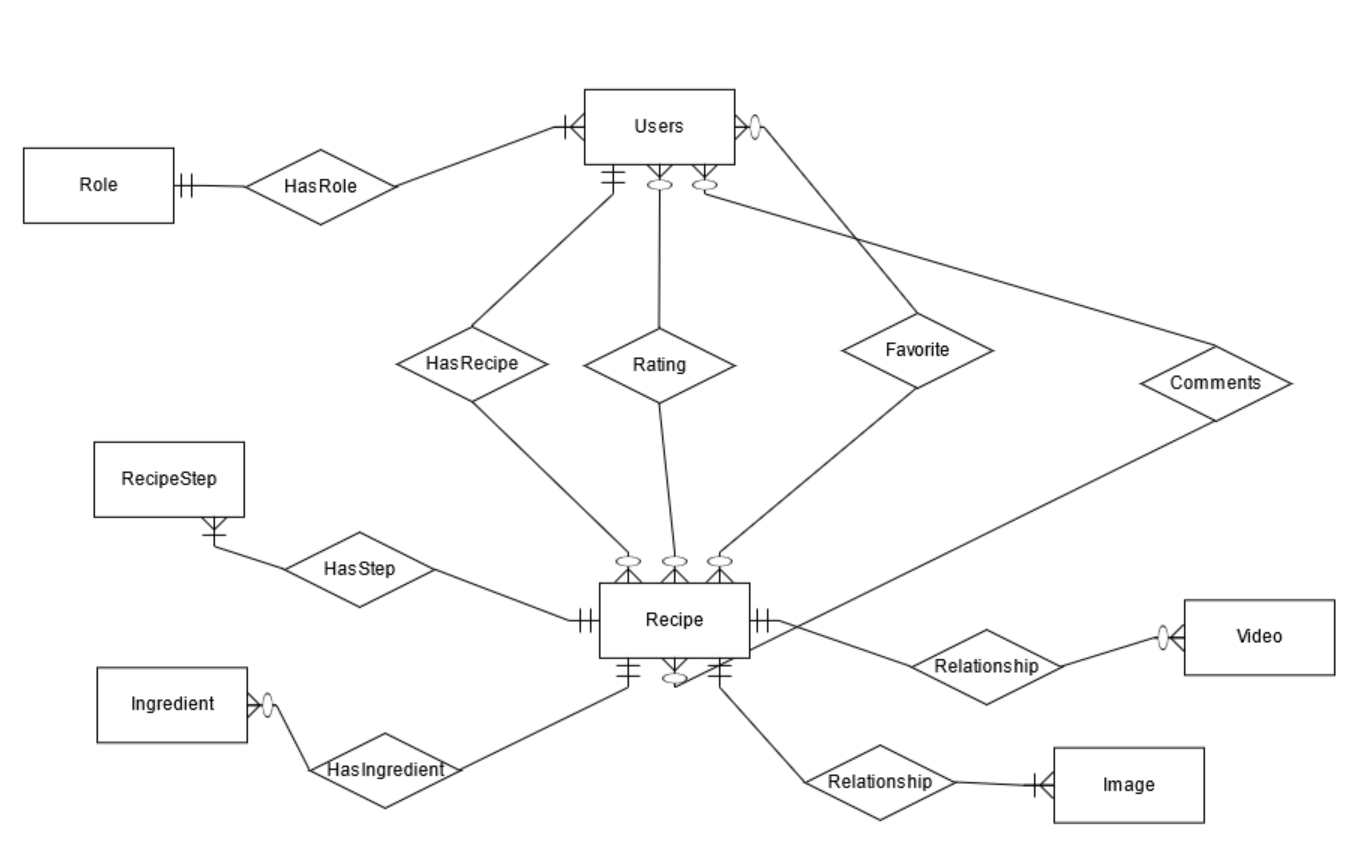
\includegraphics[width=\textwidth,height=.25\paperheight]{ERDiagram.png}
      \caption{ERDiagram}
      \label{fig:ER Diagram}
\end{figure}
\begin{figure}[h]
      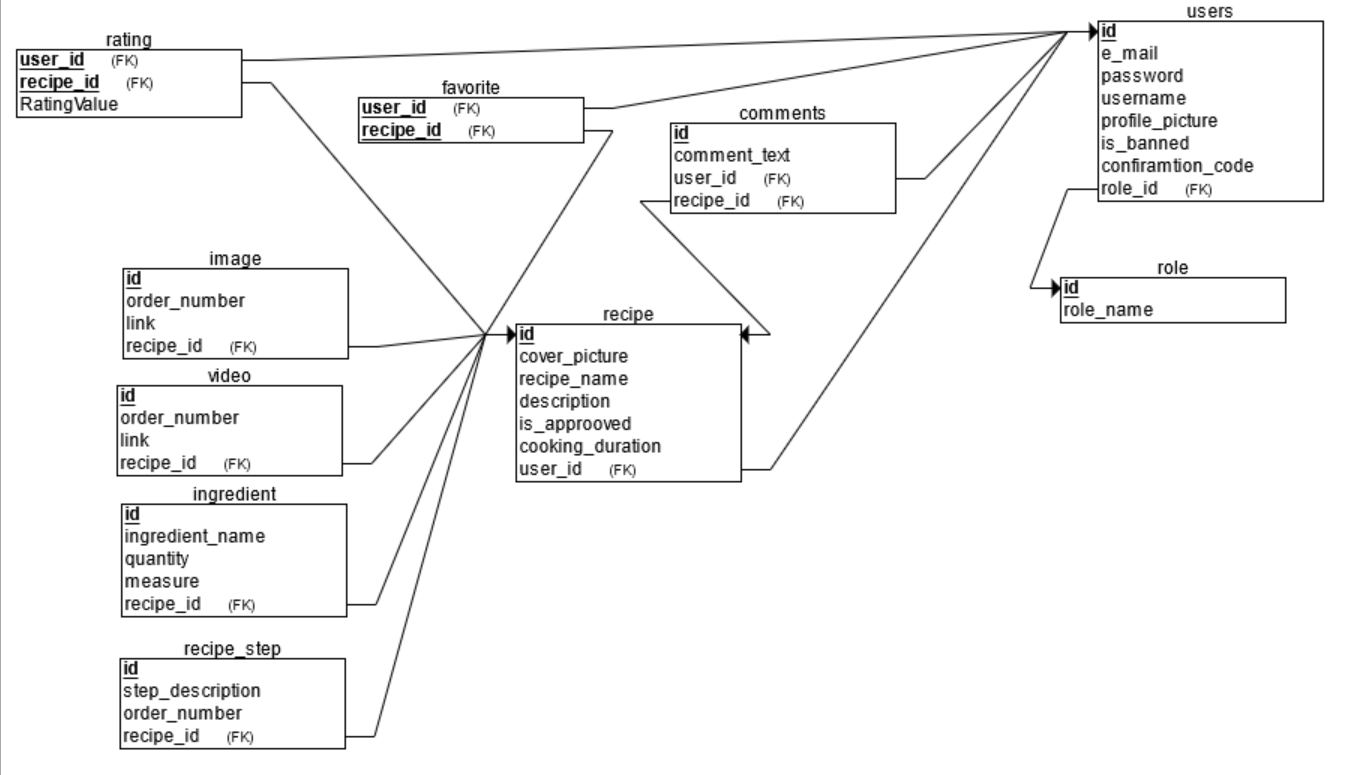
\includegraphics[width=\textwidth,height=.25\paperheight]{RelationalSchema.png}
      \caption{Relacijska shema}
      \label{fig:Relacijska shema}
\end{figure}

\chapter{Oblikovanje rješenja}
Za ispunjavanje svih zahtjeva potrebno je 9 ekrana. Svaki od njih pristupa različitoj usluzi na poslužiteljskoj strani gdje
će se provjeravati smije li trenutni korisnik pristupati tim uslugama.\\\\
Prvi ekran je prikaz dobrodošlice koji spada u nefunkcionalne zahtjeve i dodan je kao
estetski detalj te ne šalje nikakve upite (slika \ref*{fig:WelcomeLogin} (a)).\\
Drugi ekran namijenjen je za prijavu u aplikaciju te pristupa usluzi za prijavu u sustav
na poslužitelju (slika \ref*{fig:WelcomeLogin} (a) i (b)).
\begin{figure}[h]
      \centering
      \subfloat[\centering Ekran dobrodošlice]{{
\includegraphics[width=.26\textwidth]{welcome_screen.jpg} }}
      \subfloat[\centering Ekran prijave]{{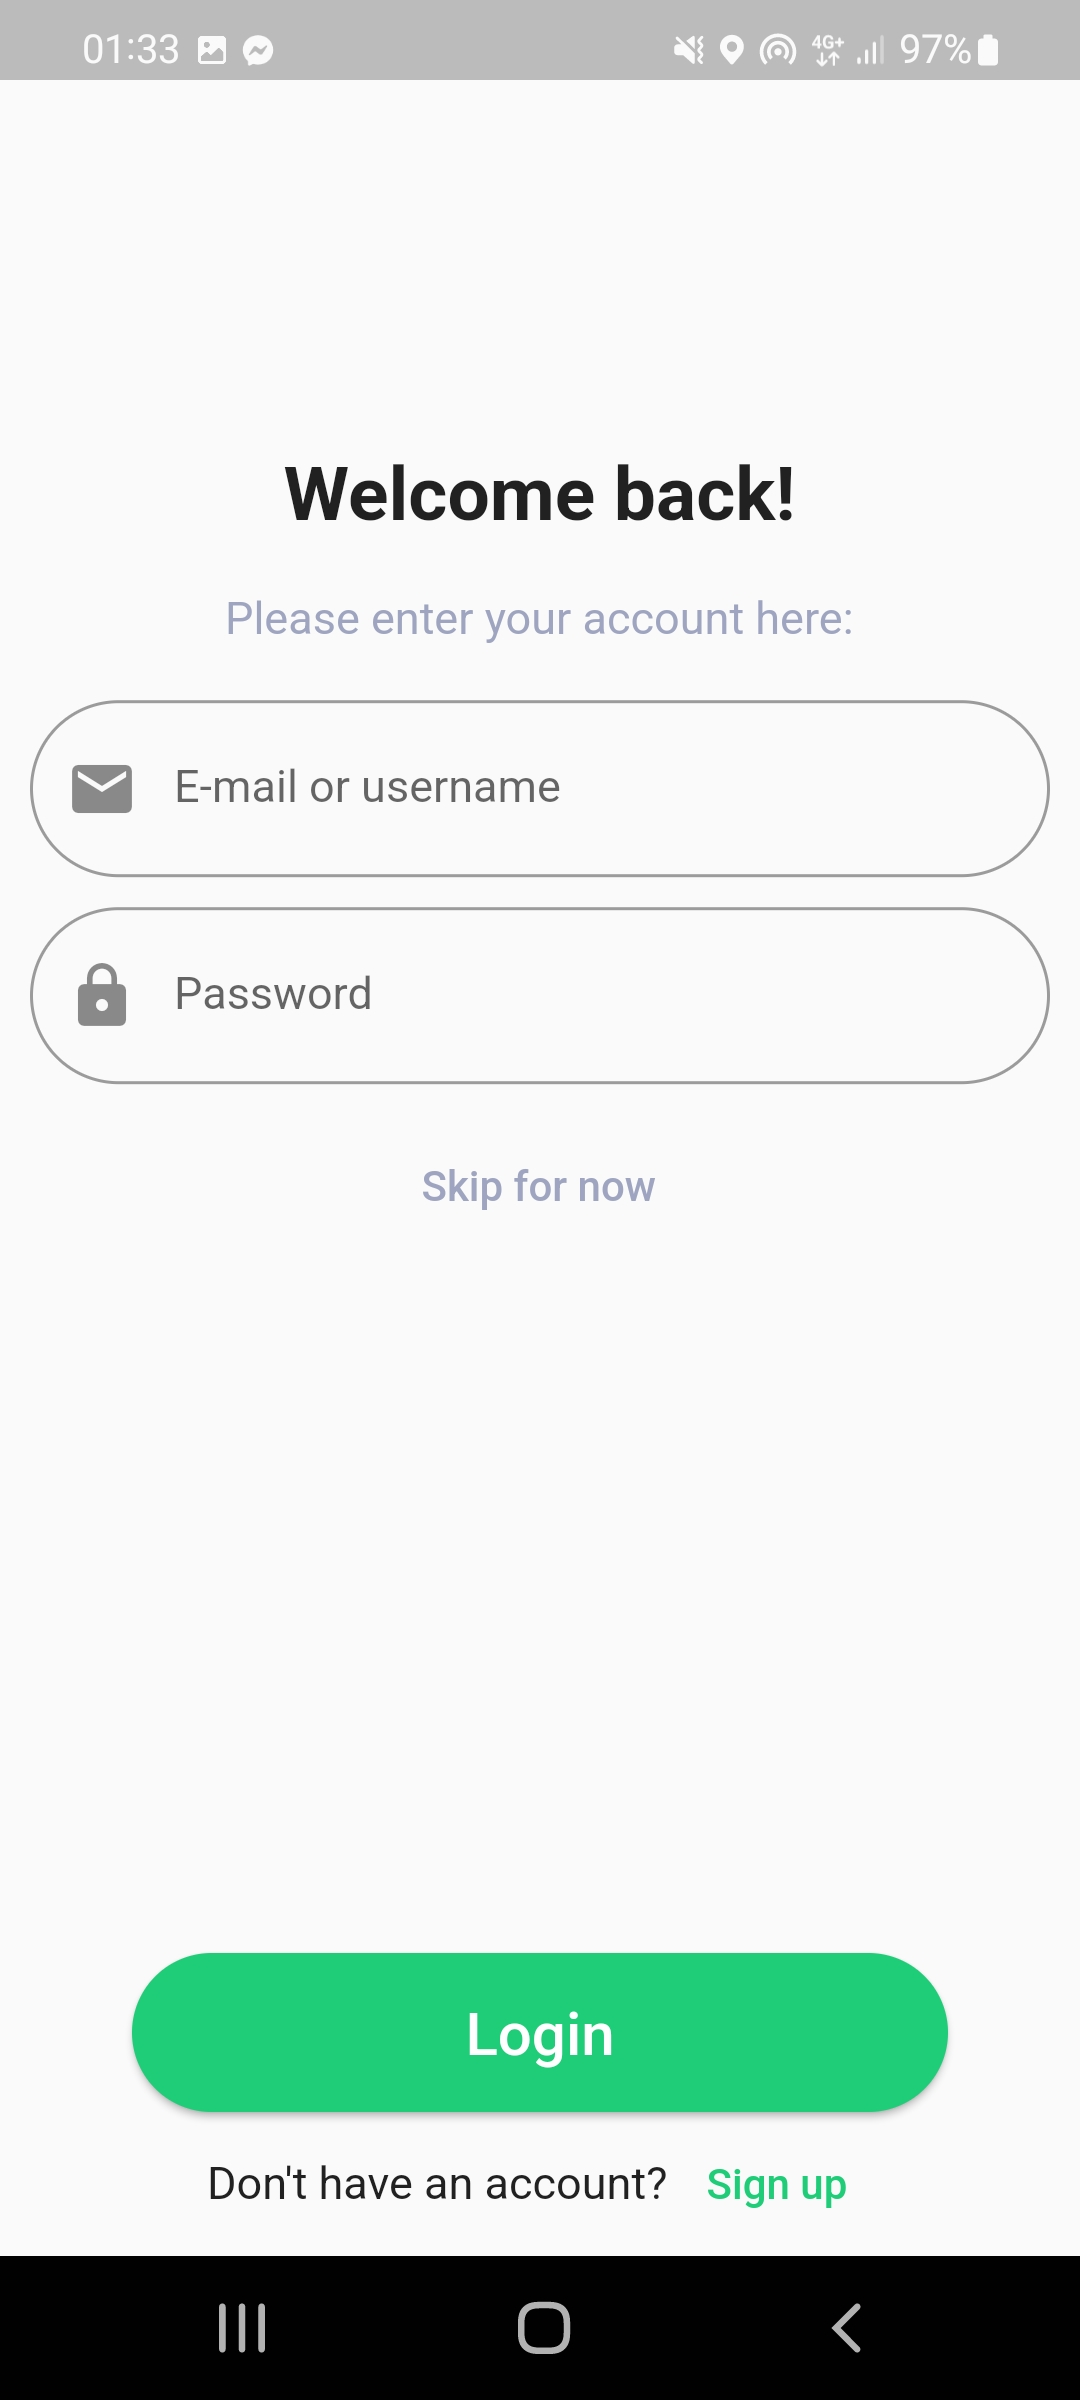
\includegraphics[width=.26\textwidth]{login_screen.jpg} }}
      \subfloat[\centering Ekran prijave u slučaju pogreške]{{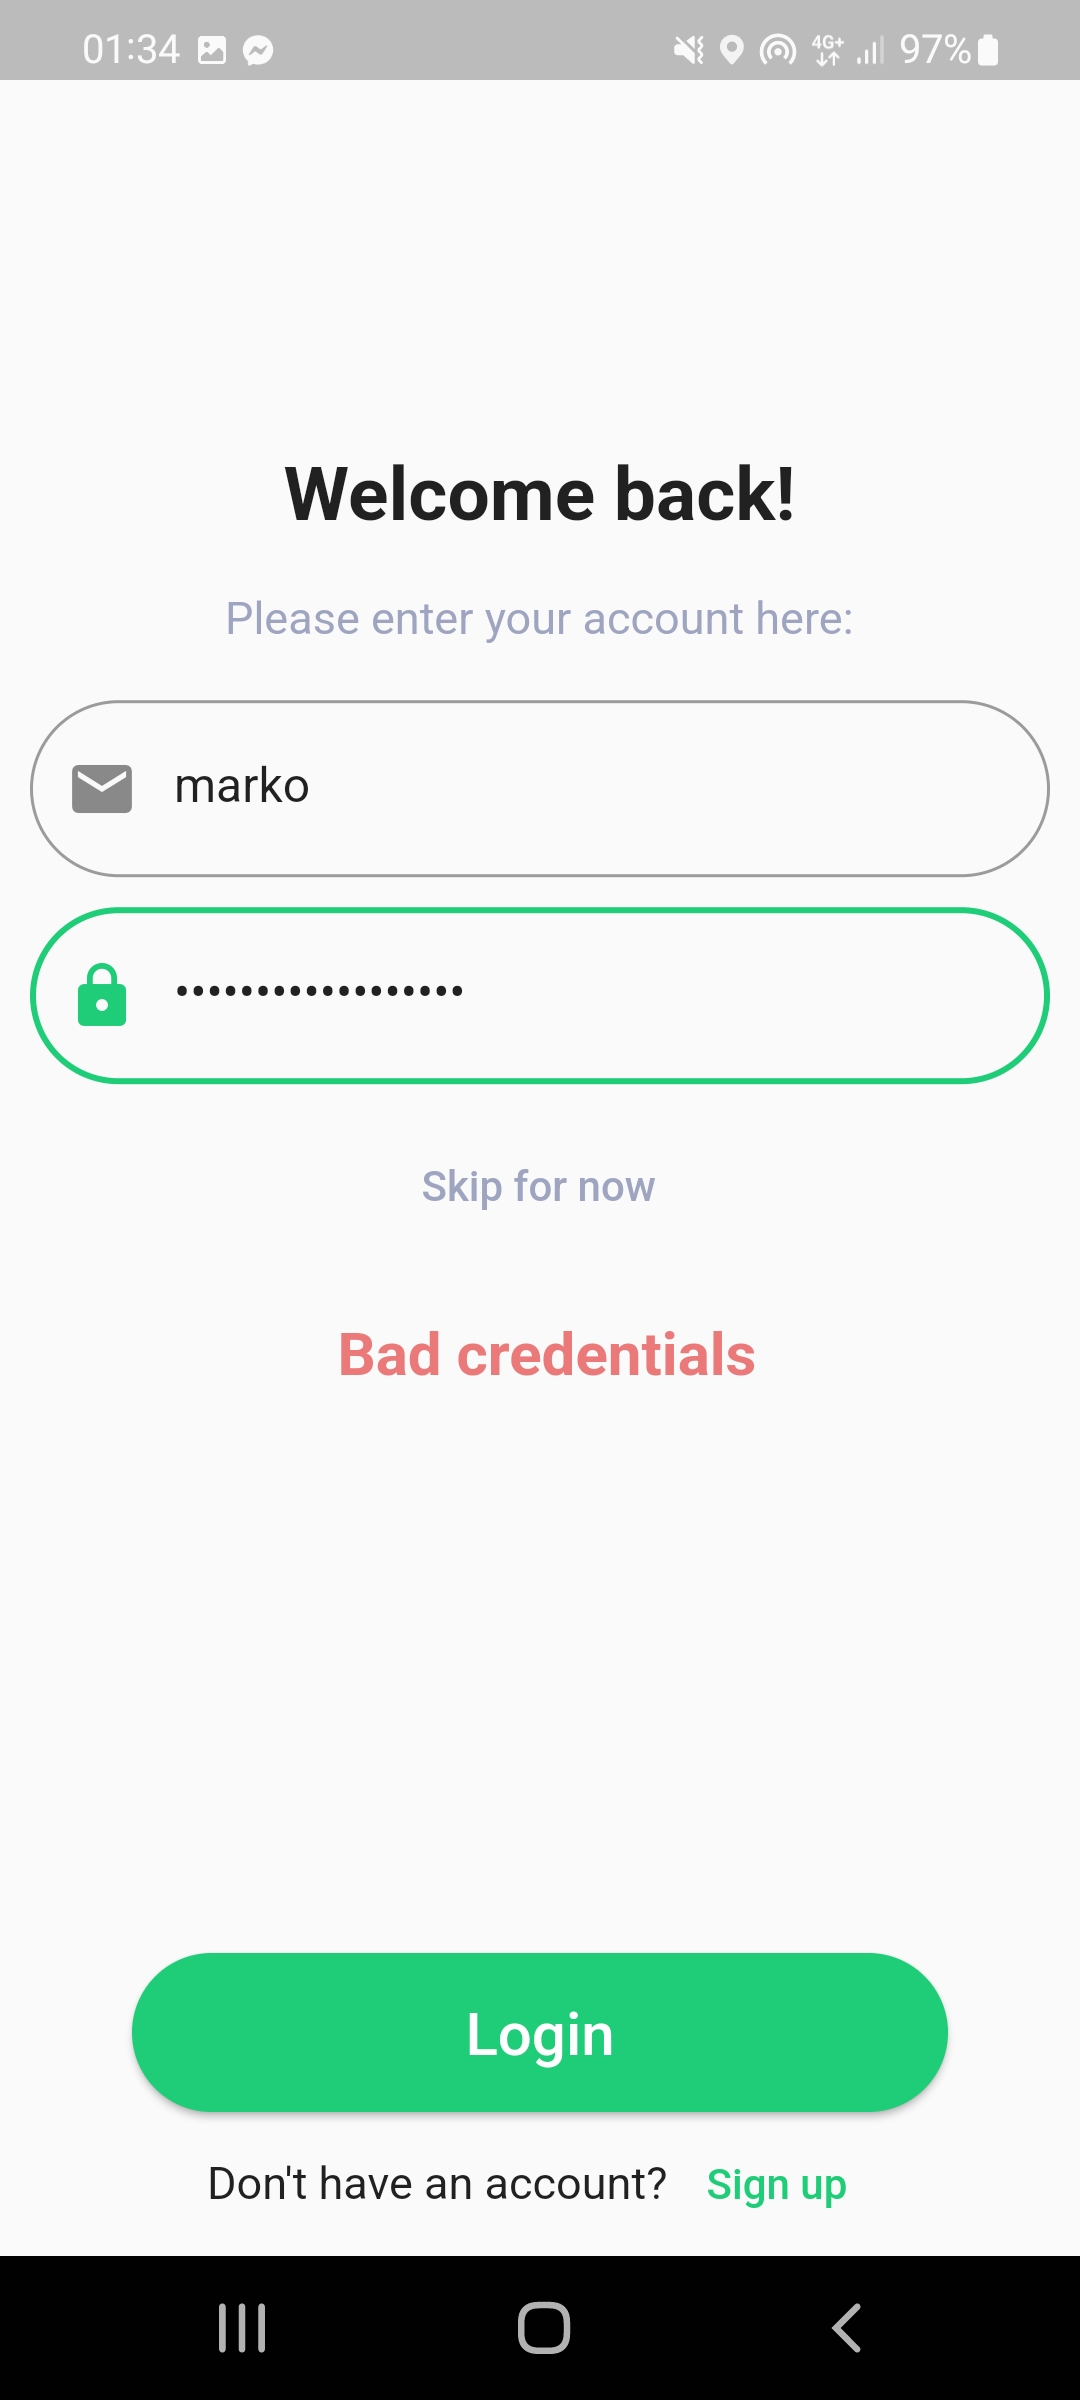
\includegraphics[width=.26\textwidth]{login_failed.jpg} }}
      \caption{Ekran dobrodošlice i prijave}
      \label{fig:WelcomeLogin}
\end{figure}\newpage
Treći ekran služi za registraciju u sustav. Na njemu će korisnik unositi zahtjevane podatke i
poslati ih poslužitelju. Poslužitelj validira podatke i odgovora porukom koja može biti potvrdna i zahtjevati
od korisnika potvrdu identiteta putem elektroničke pošte ili može biti poruka pogreške koja zahtjeva promjenu unesenih
podataka (slika \ref*{fig:Register}).
\begin{figure}[h]
      \centering
      \subfloat[\centering Ekran neuspješne registracije]{{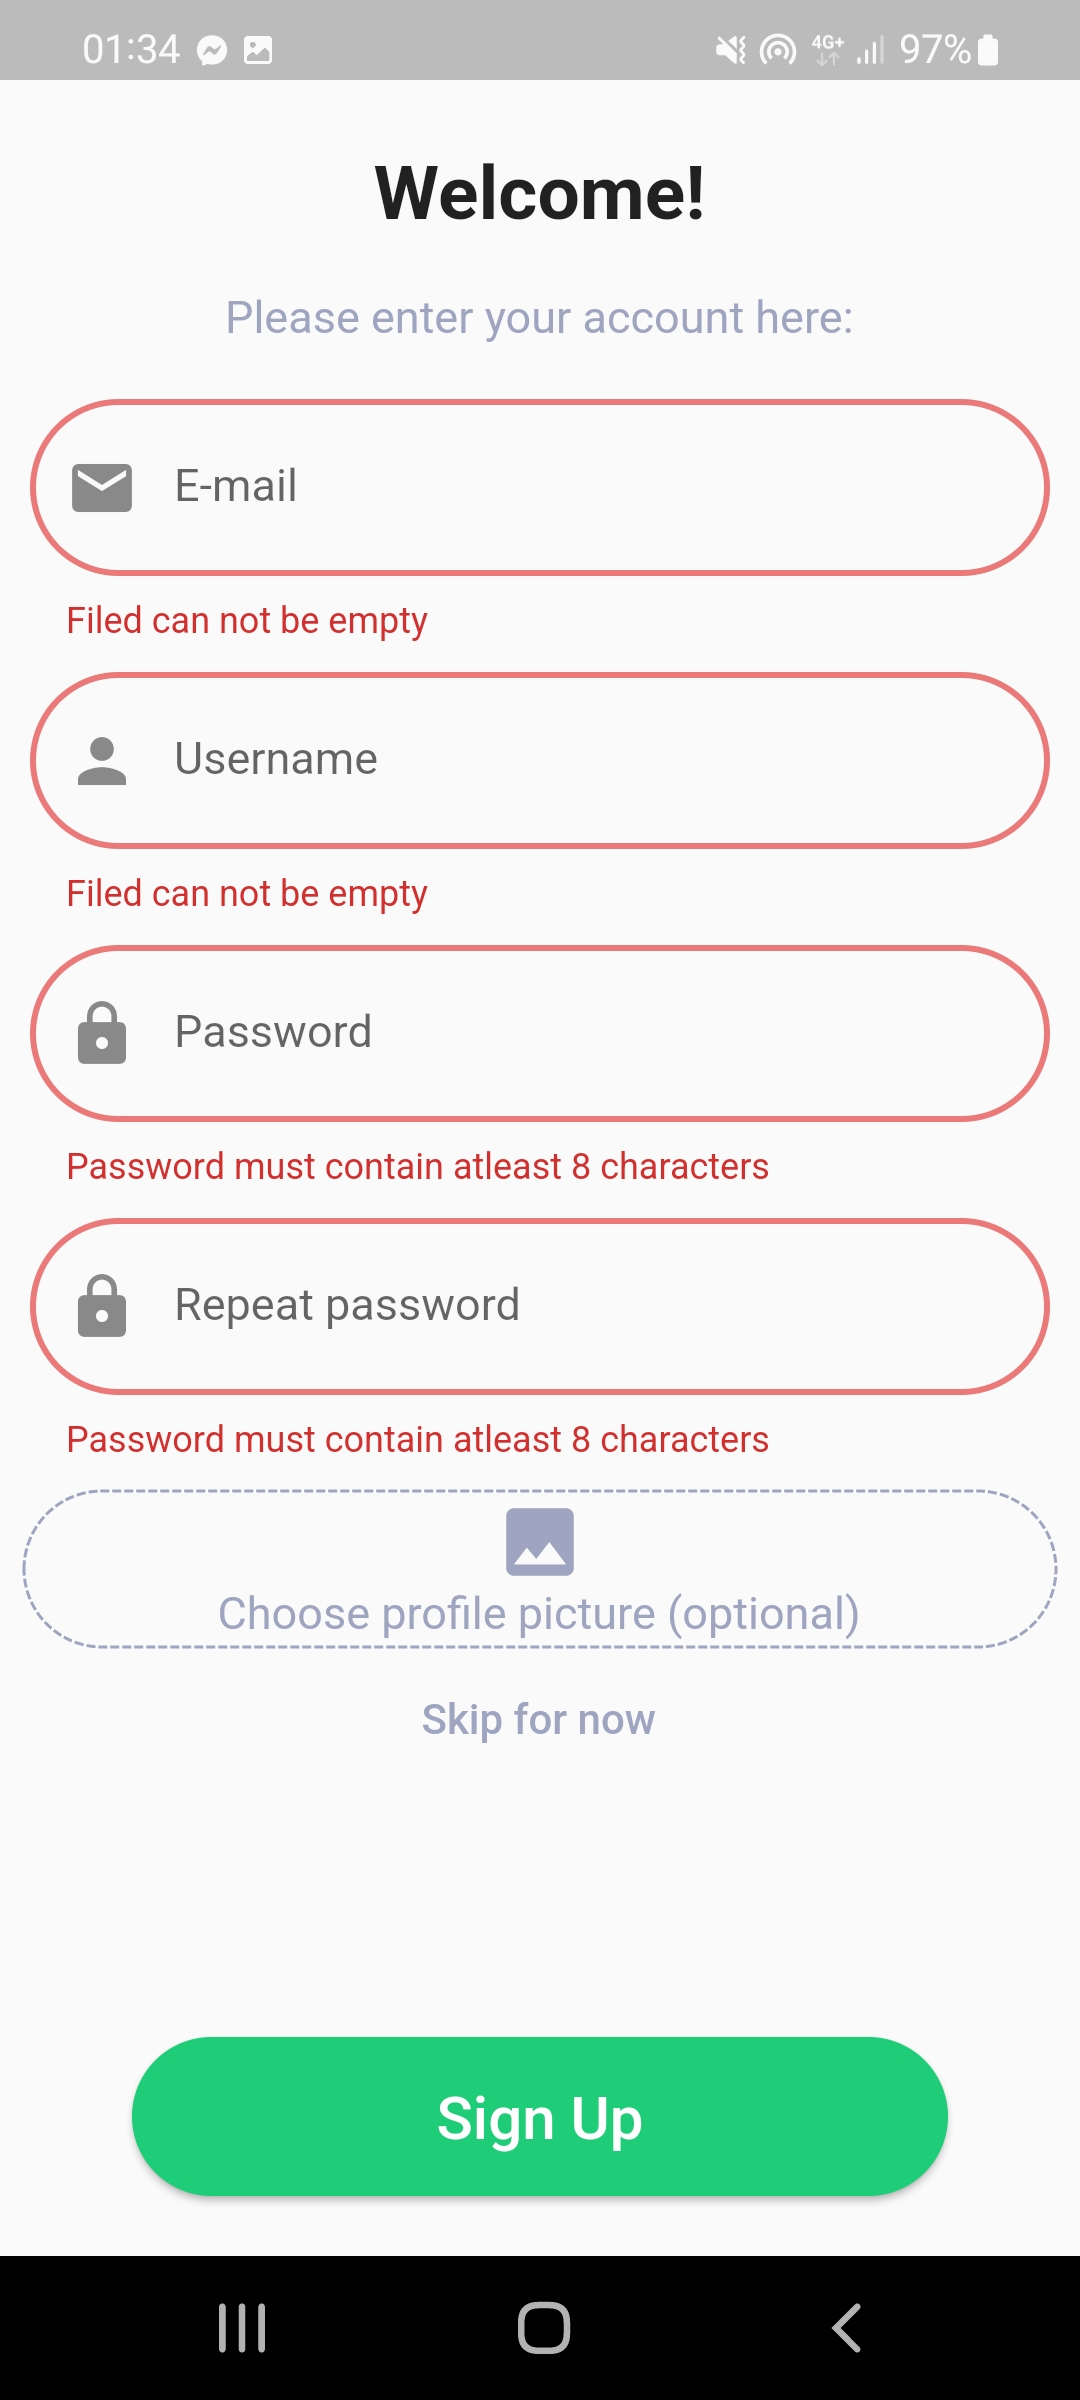
\includegraphics[width=.25\textwidth]{register_failed.jpg} }}
      \subfloat[\centering Ekran uspješne registracije]{{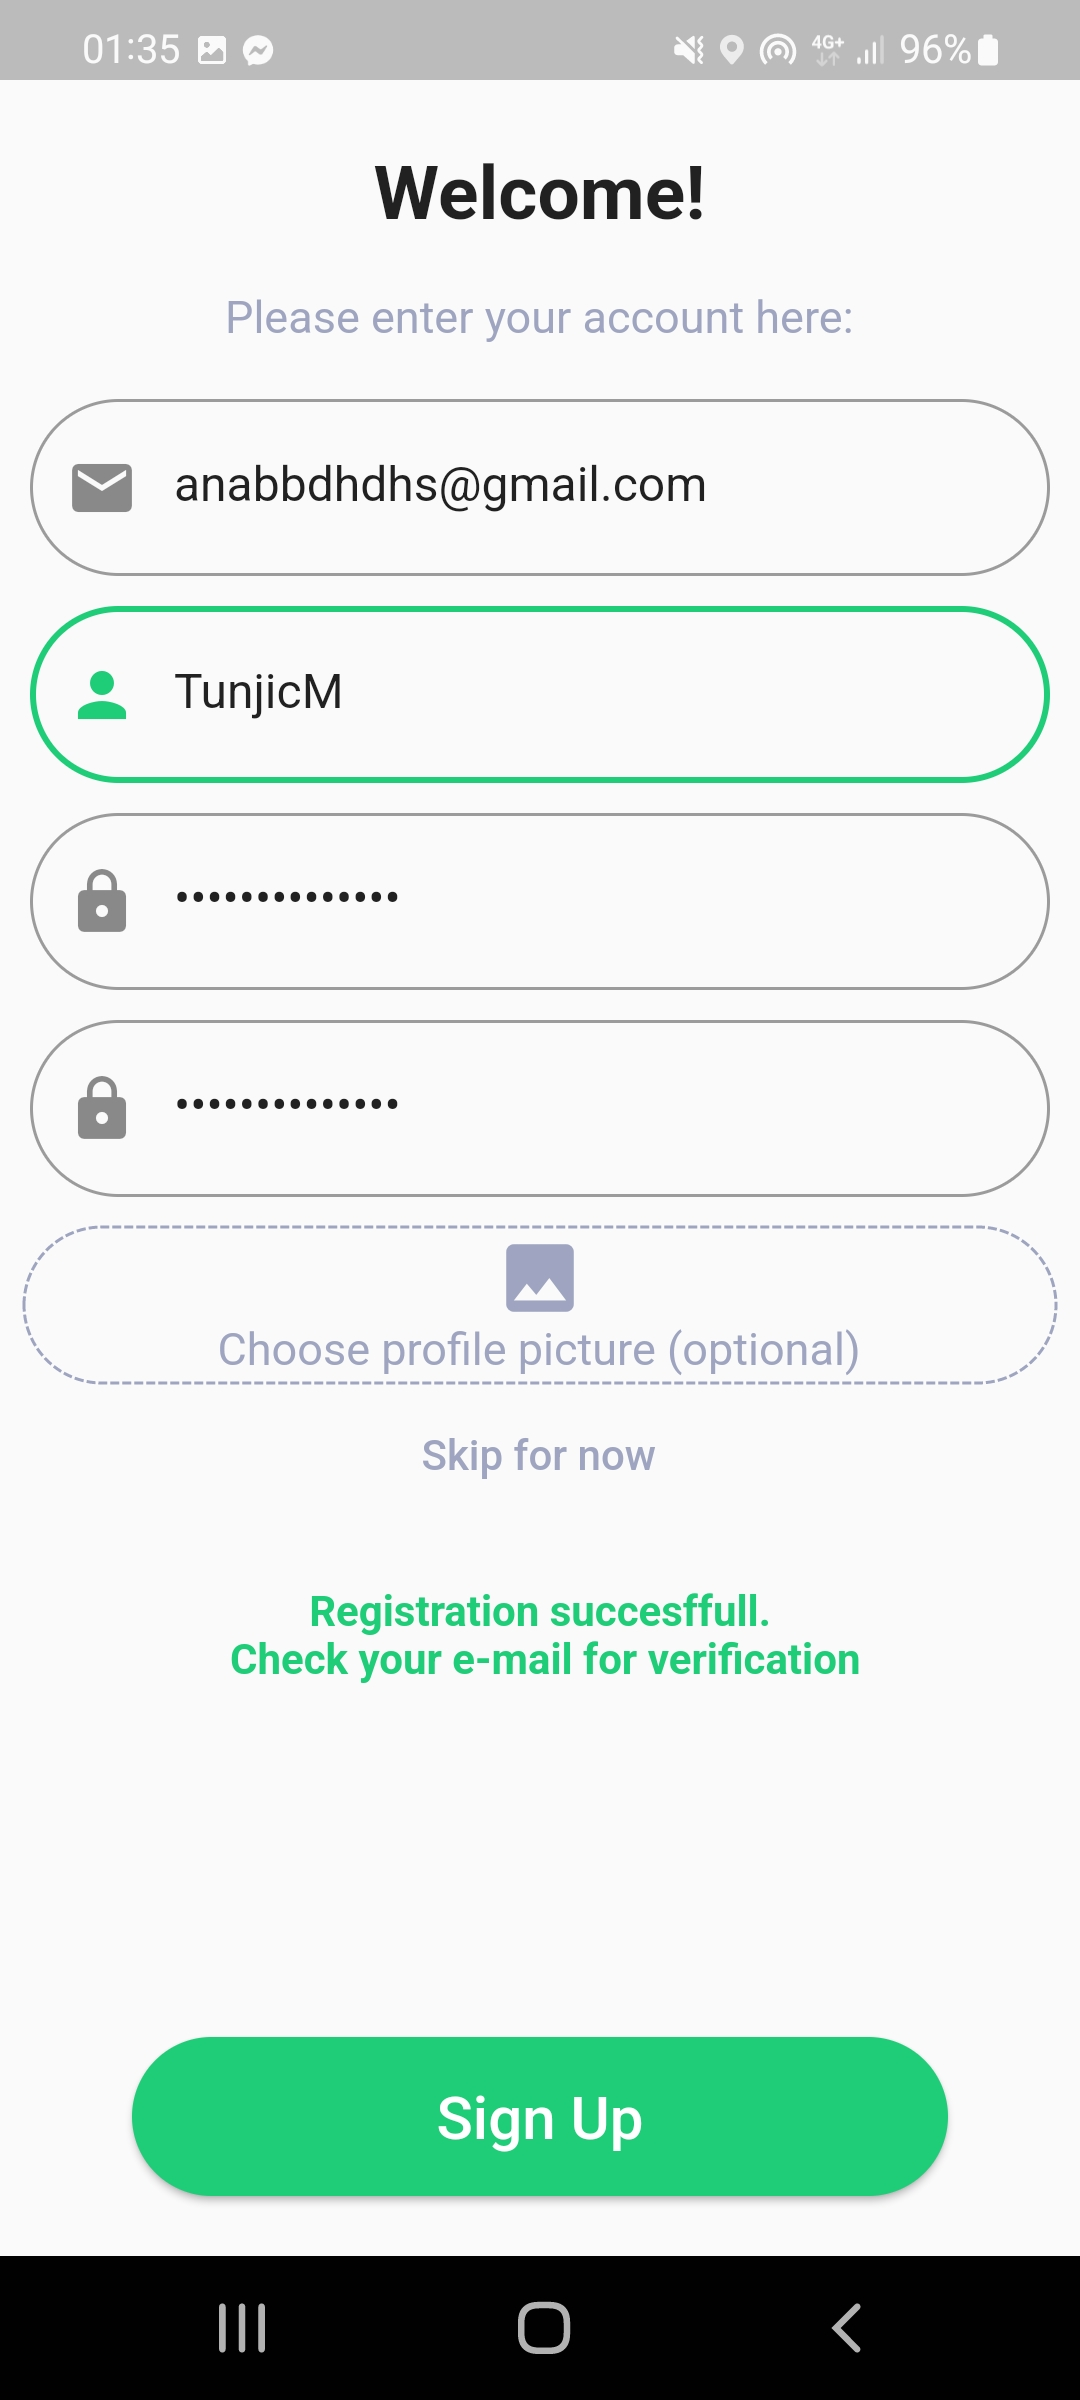
\includegraphics[width=.25\textwidth]{register_success.jpg} }}
      \caption{Ekrani za registraciju}
      \label{fig:Register}
\end{figure}\\
Na četvrtom ekranu se nalaze svi recepti koji postoje u bazi podataka i elementi koji služe za
filtriranje recepata i dodavanje recepata u favorite.
Ovaj ekran od poslužitelja zahtjeva sve recepte koji zadovoljavaju odabrani
filter. Taj filter može biti prazan (u slučaju zahtjevanja svih recepata) ili popunjen zahtjevanim nazivom
i/ili sastojcima koji smiju odnosno ne smiju biti sadržani u receptu (slika \ref*{fig:All recipes}).
\begin{figure}[h]
      \centering
      \subfloat[\centering Ekran sa svim receptima]{{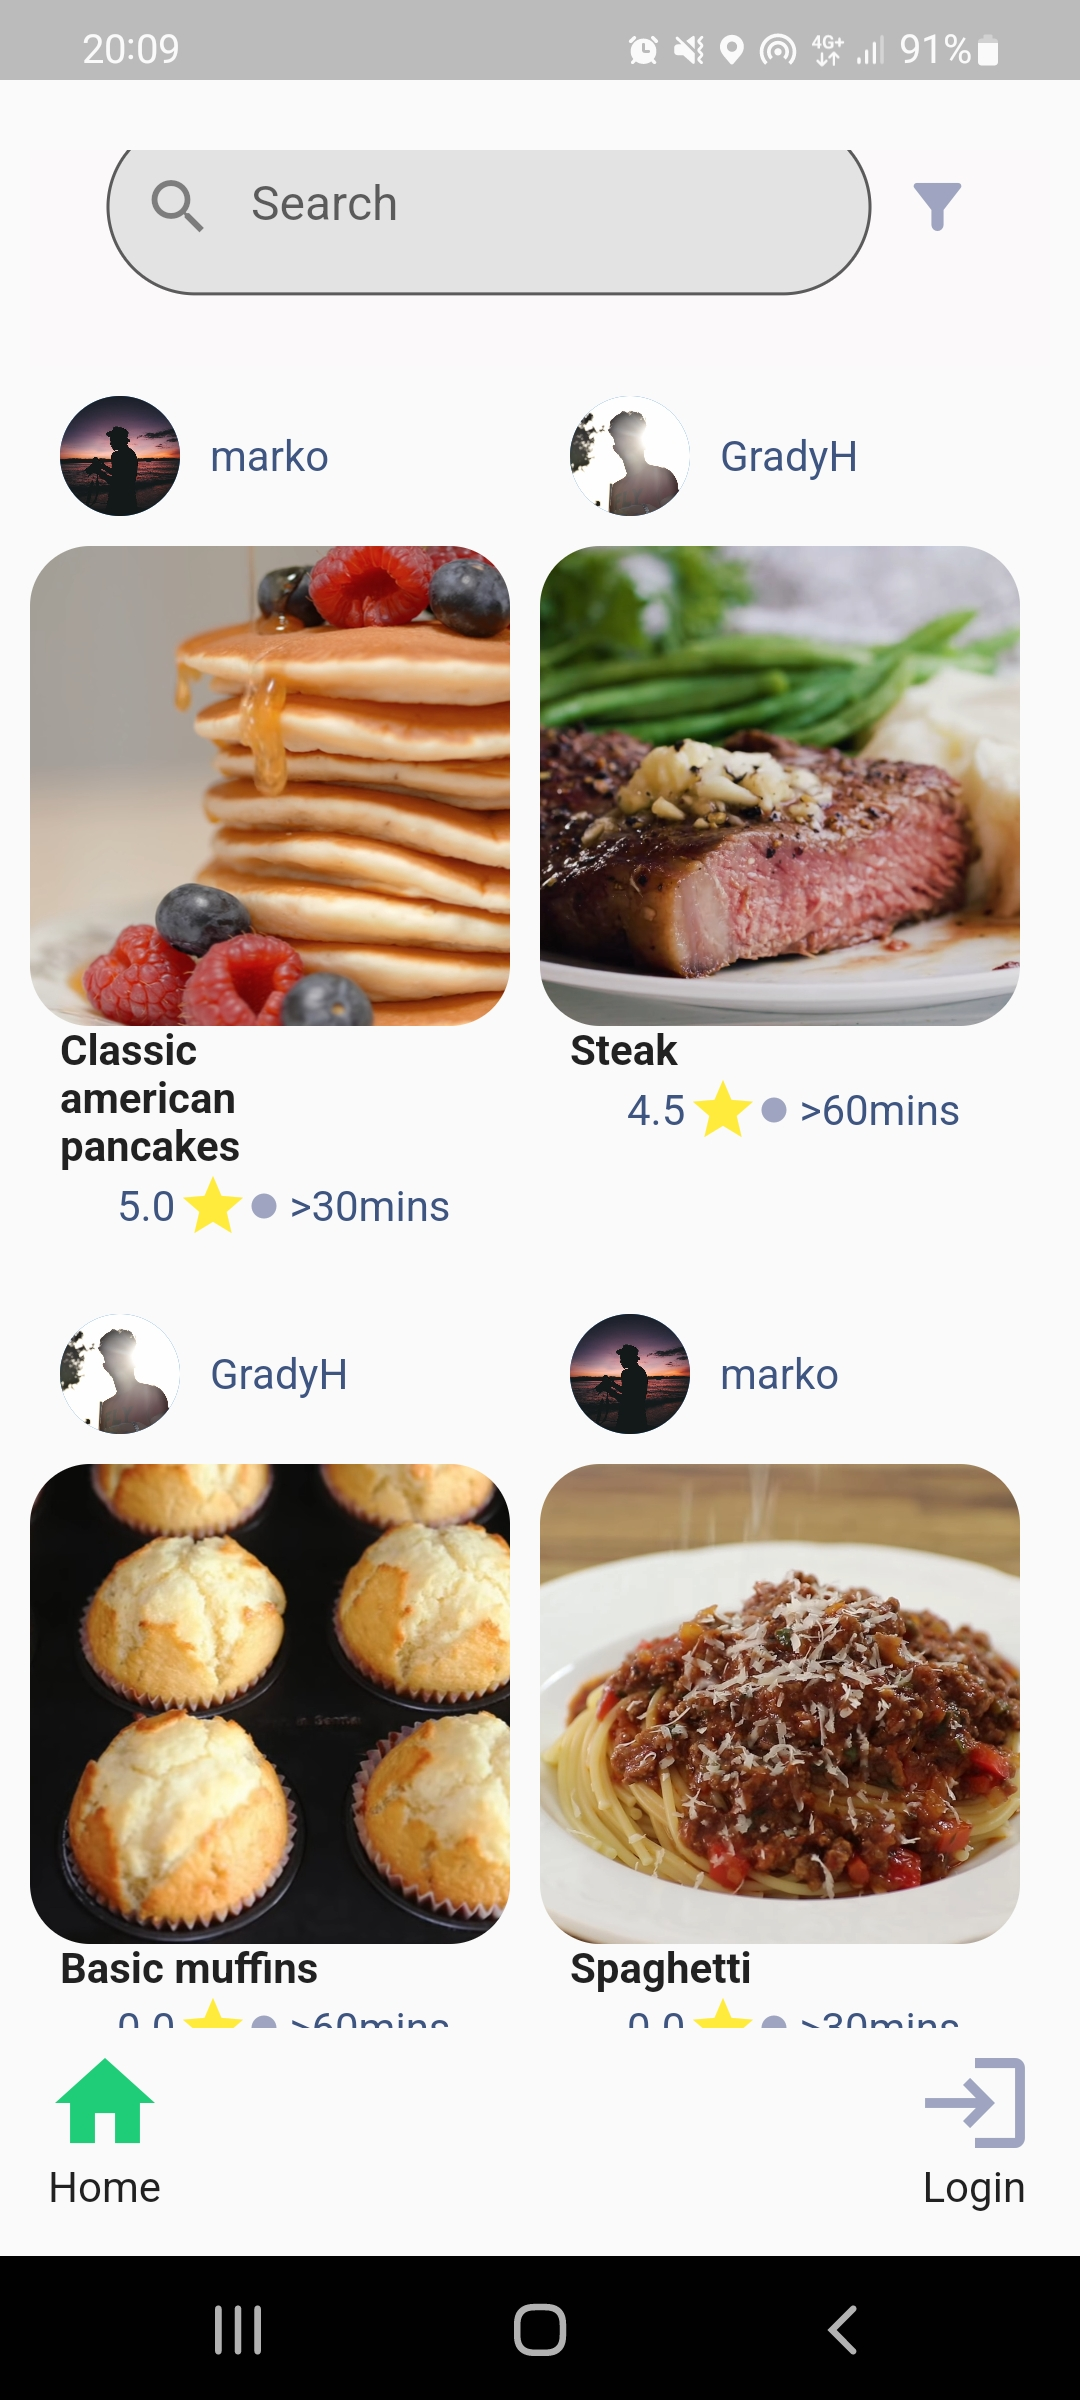
\includegraphics[width=.25\textwidth]{not_loggedin.jpg} }}
      \subfloat[\centering Dijalog za filtriranje]{{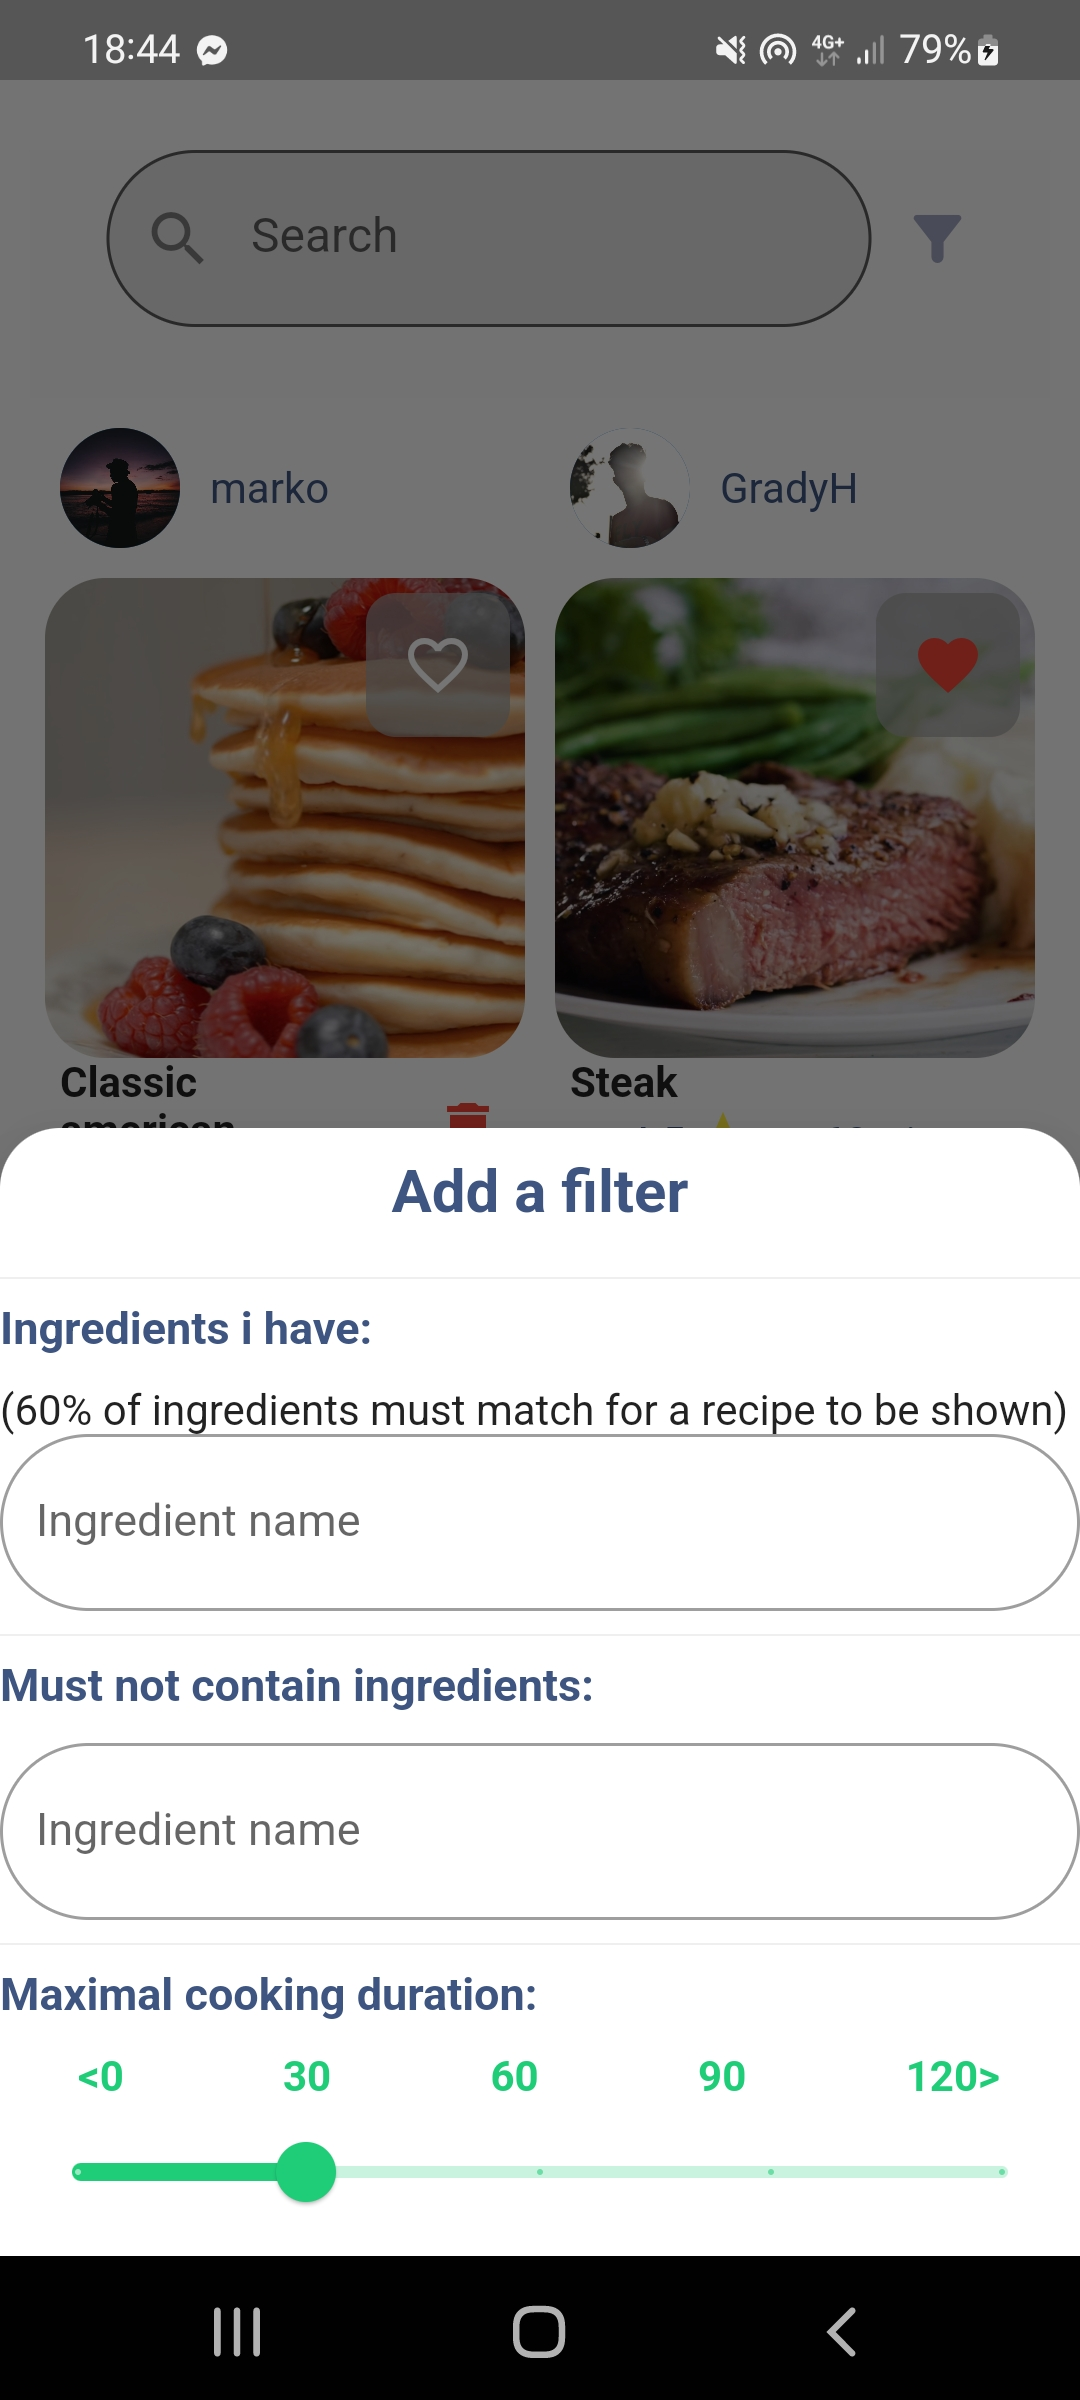
\includegraphics[width=.25\textwidth]{filter.jpg} }}
      \caption{Ekran sa receptima}
      \label{fig:All recipes}
\end{figure}\\
Peti ekran je formular za unos novog recepta na kojem postoje elementi za dodavanje
obveznih podataka o receptu kao na primjer naziv, opis, koraci i slično. Također postoje elementi za odabir fotografija i/ili
videozapisa. Ti podaci će isto kao i oni za registraciju biti poslani poslužitelju koji ih validira i odgovara
porukom o uspješnosti dodavanja recepta (slika \ref*{fig:New recipe} (a) i (b)).
\begin{figure}[h]
      \centering
      \subfloat[\centering Prvi dio ekrana za dodavanje recepta]{{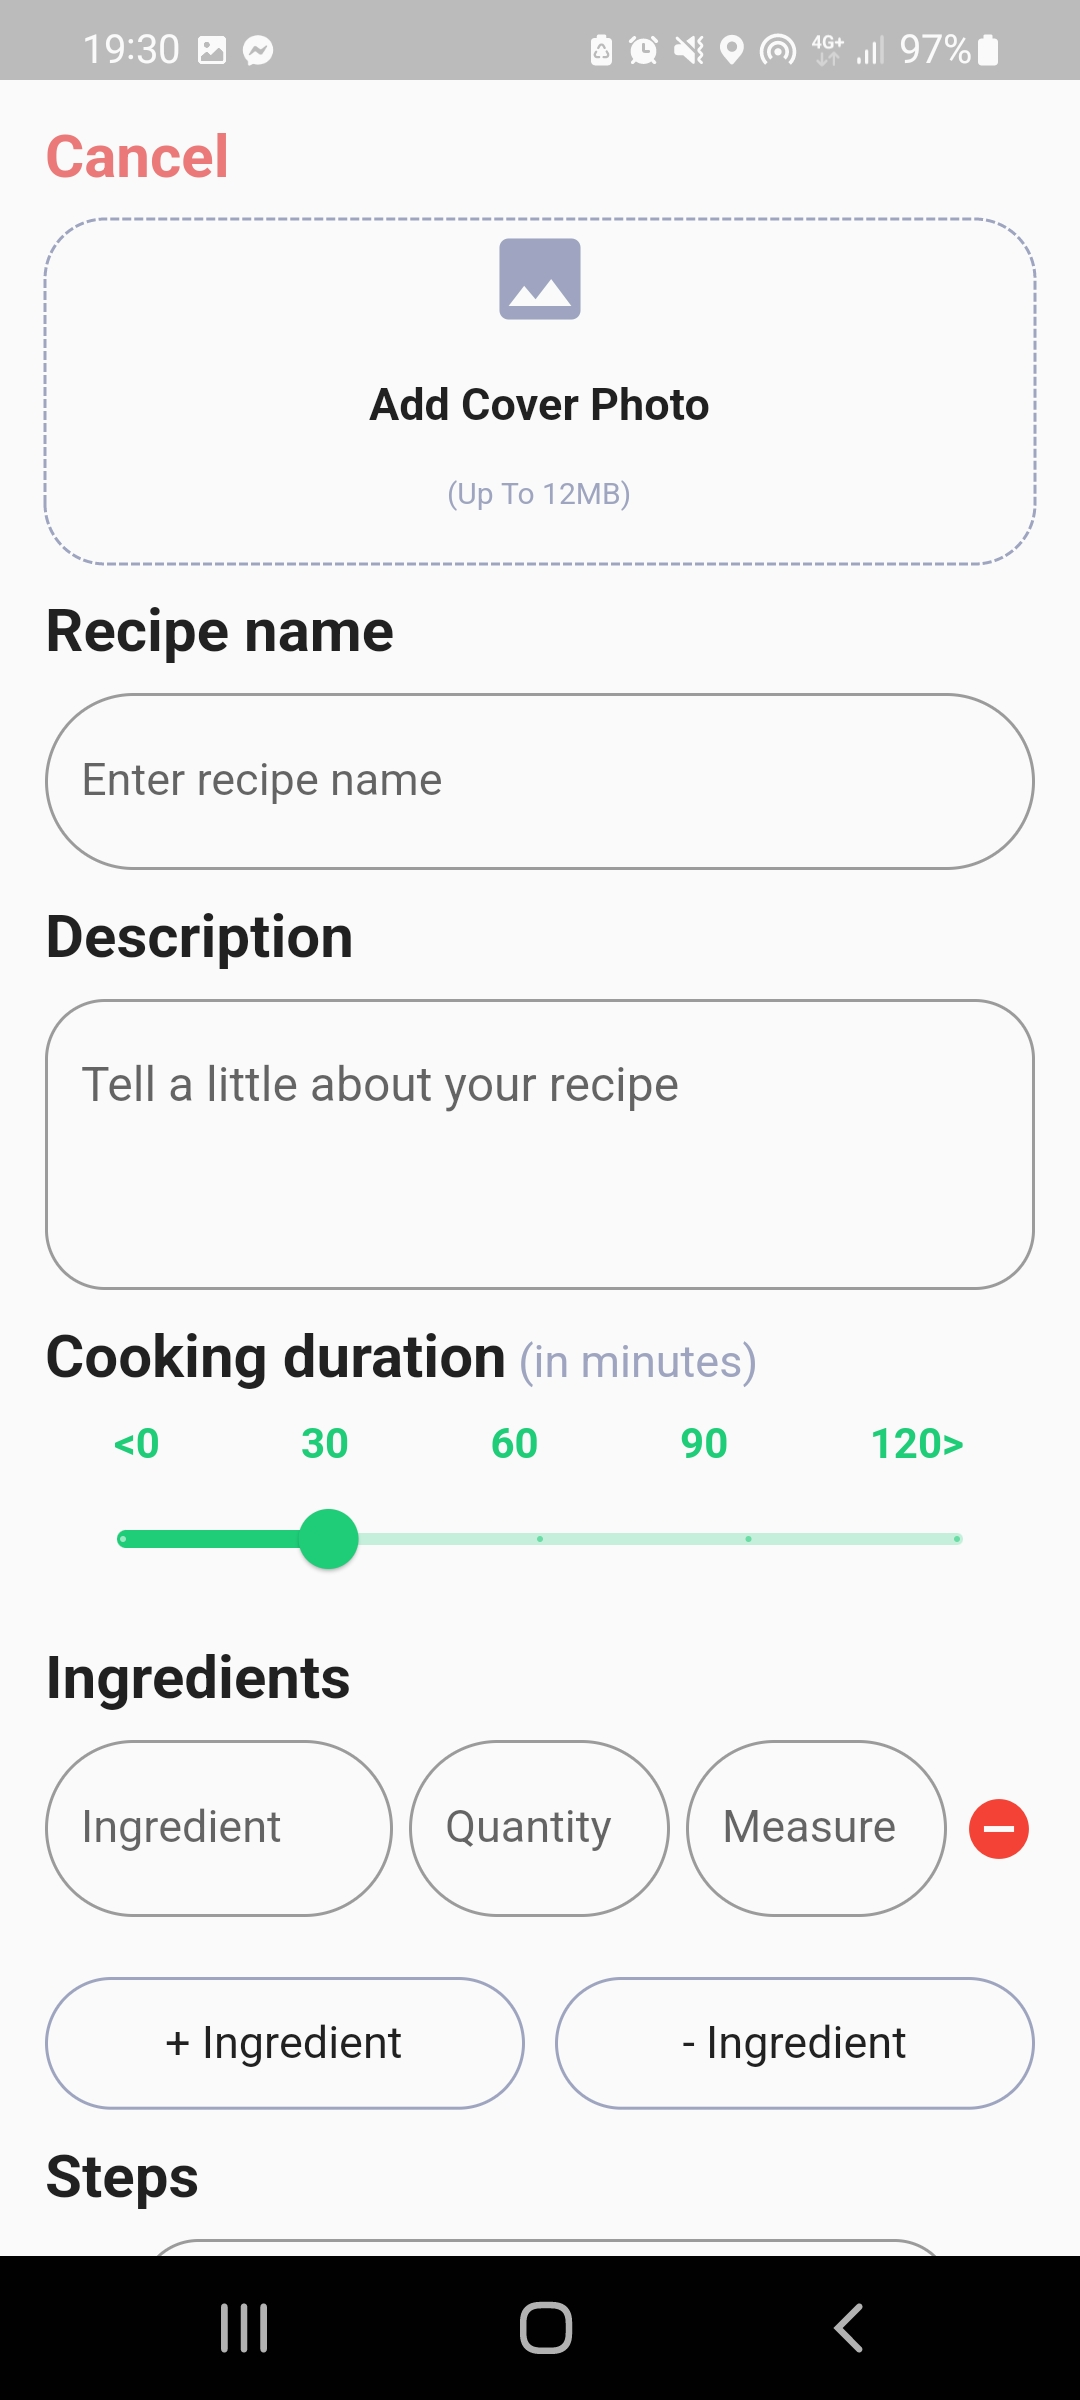
\includegraphics[width=.25\textwidth]{new_recipe1.jpg} }}
      \subfloat[\centering Drugi dio ekrana za dodavanje recepta]{{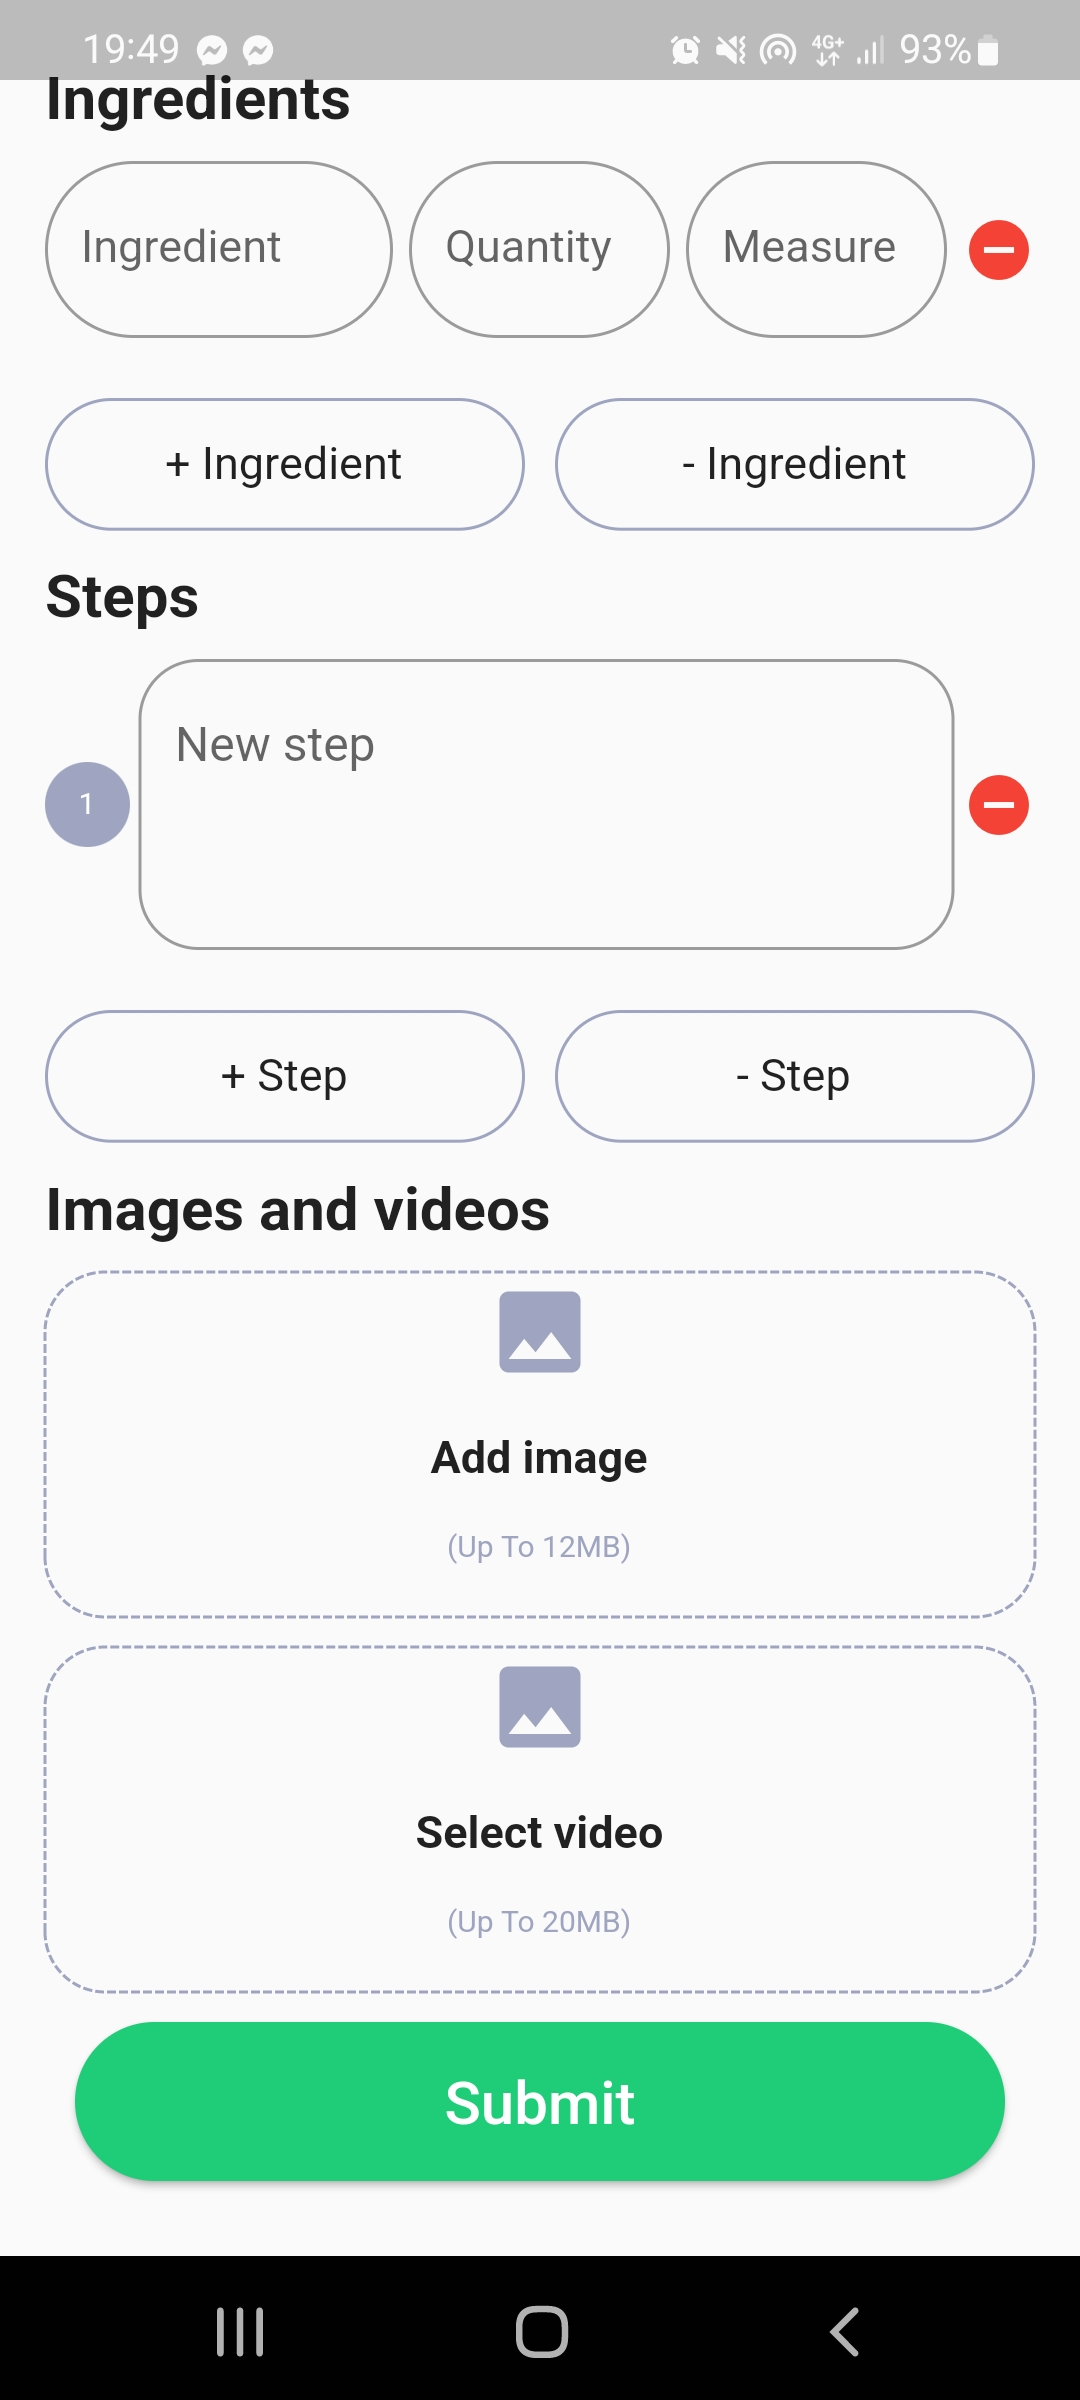
\includegraphics[width=.25\textwidth]{new_recipe2.jpg} }}
      \subfloat[\centering Prvi dio ekrana za detalje o receptu]{{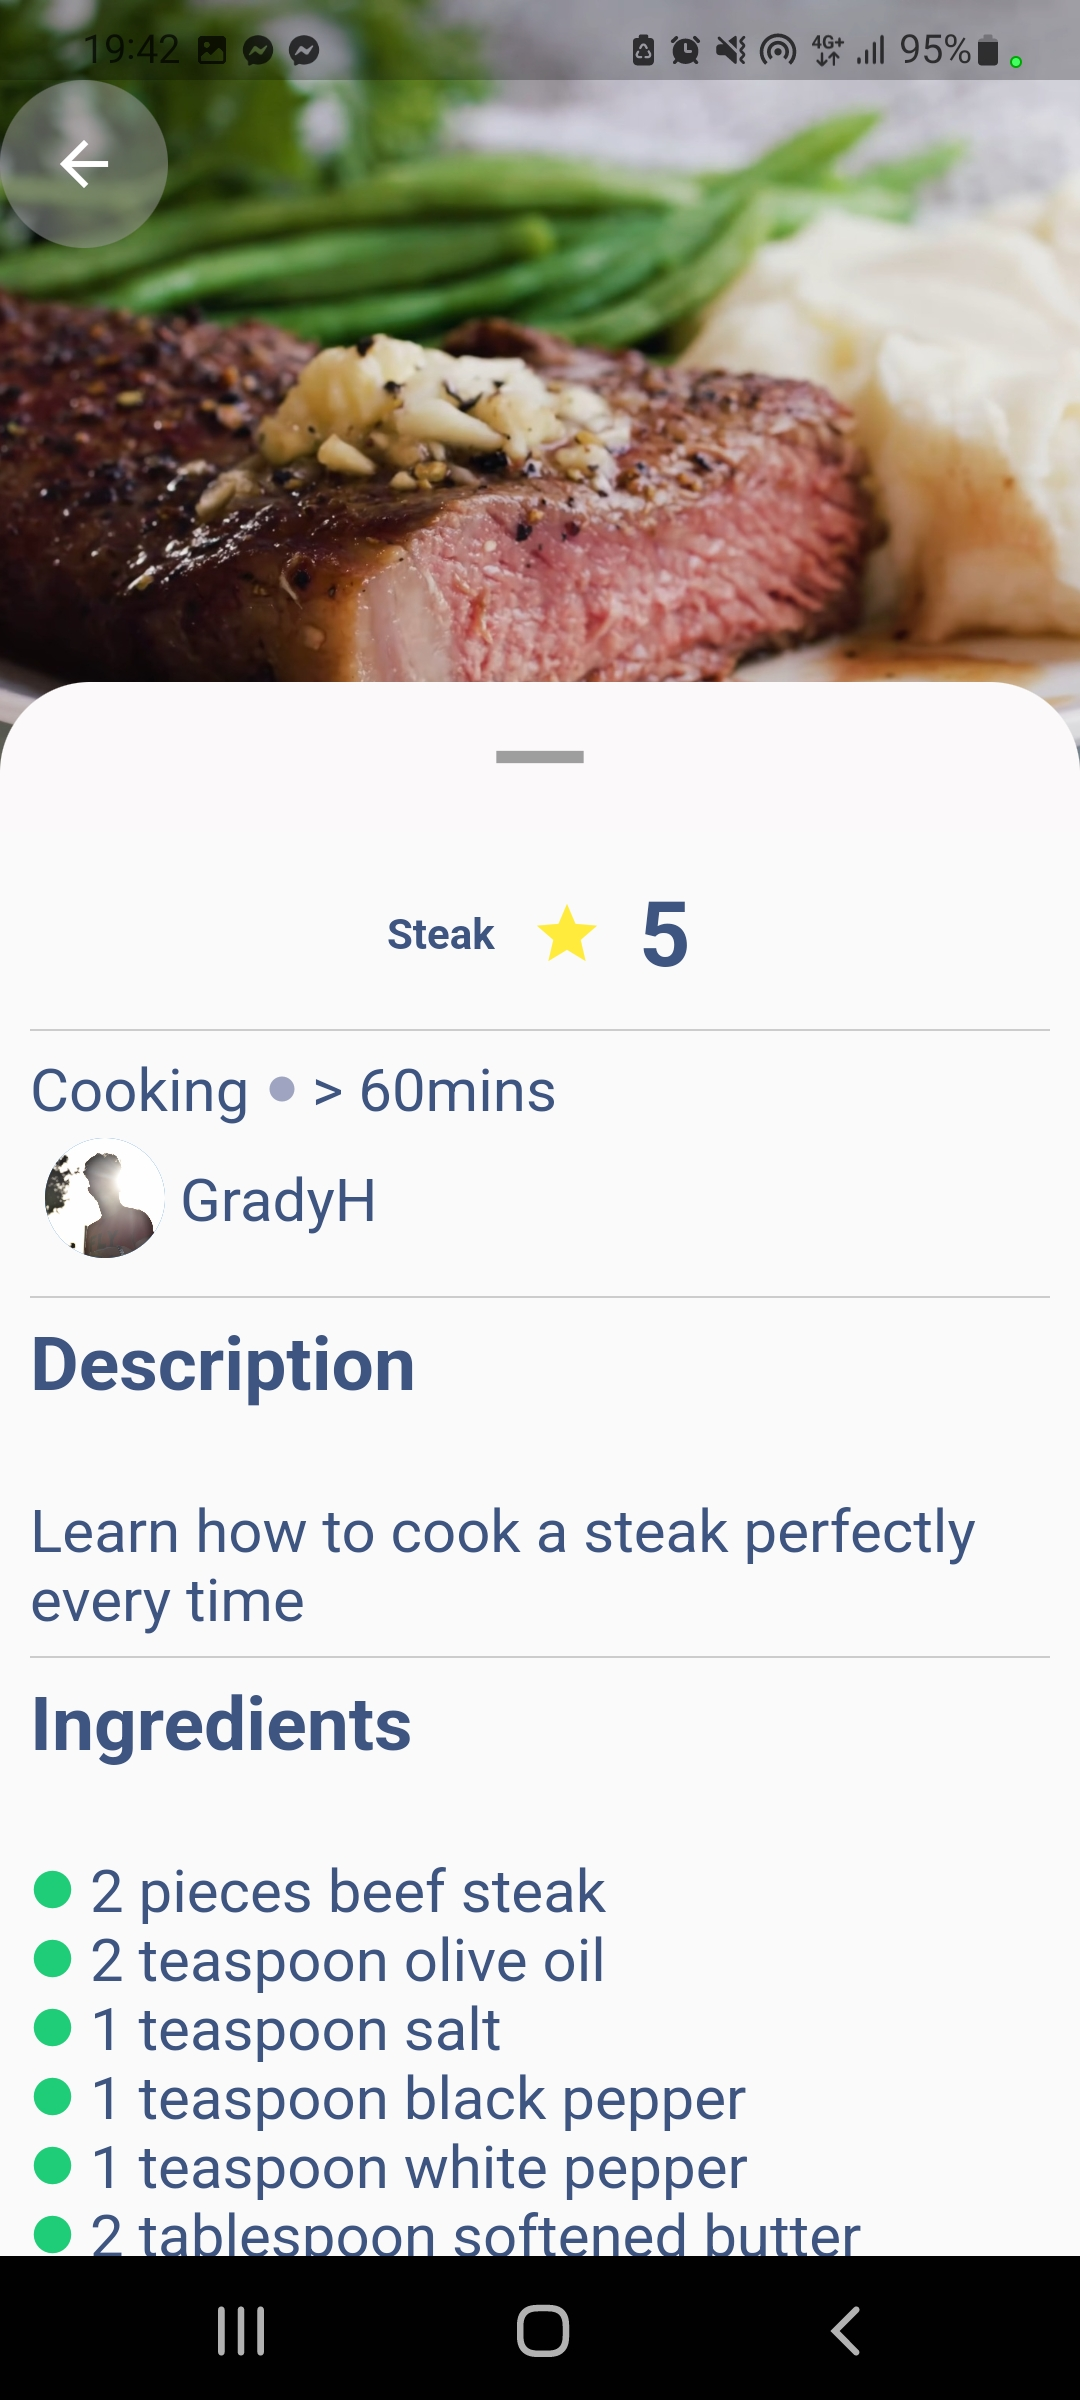
\includegraphics[width=.25\textwidth]{single_recipe_user.jpg} }}
      \subfloat[\centering Drugi dio ekrana za detalje o receptu]{{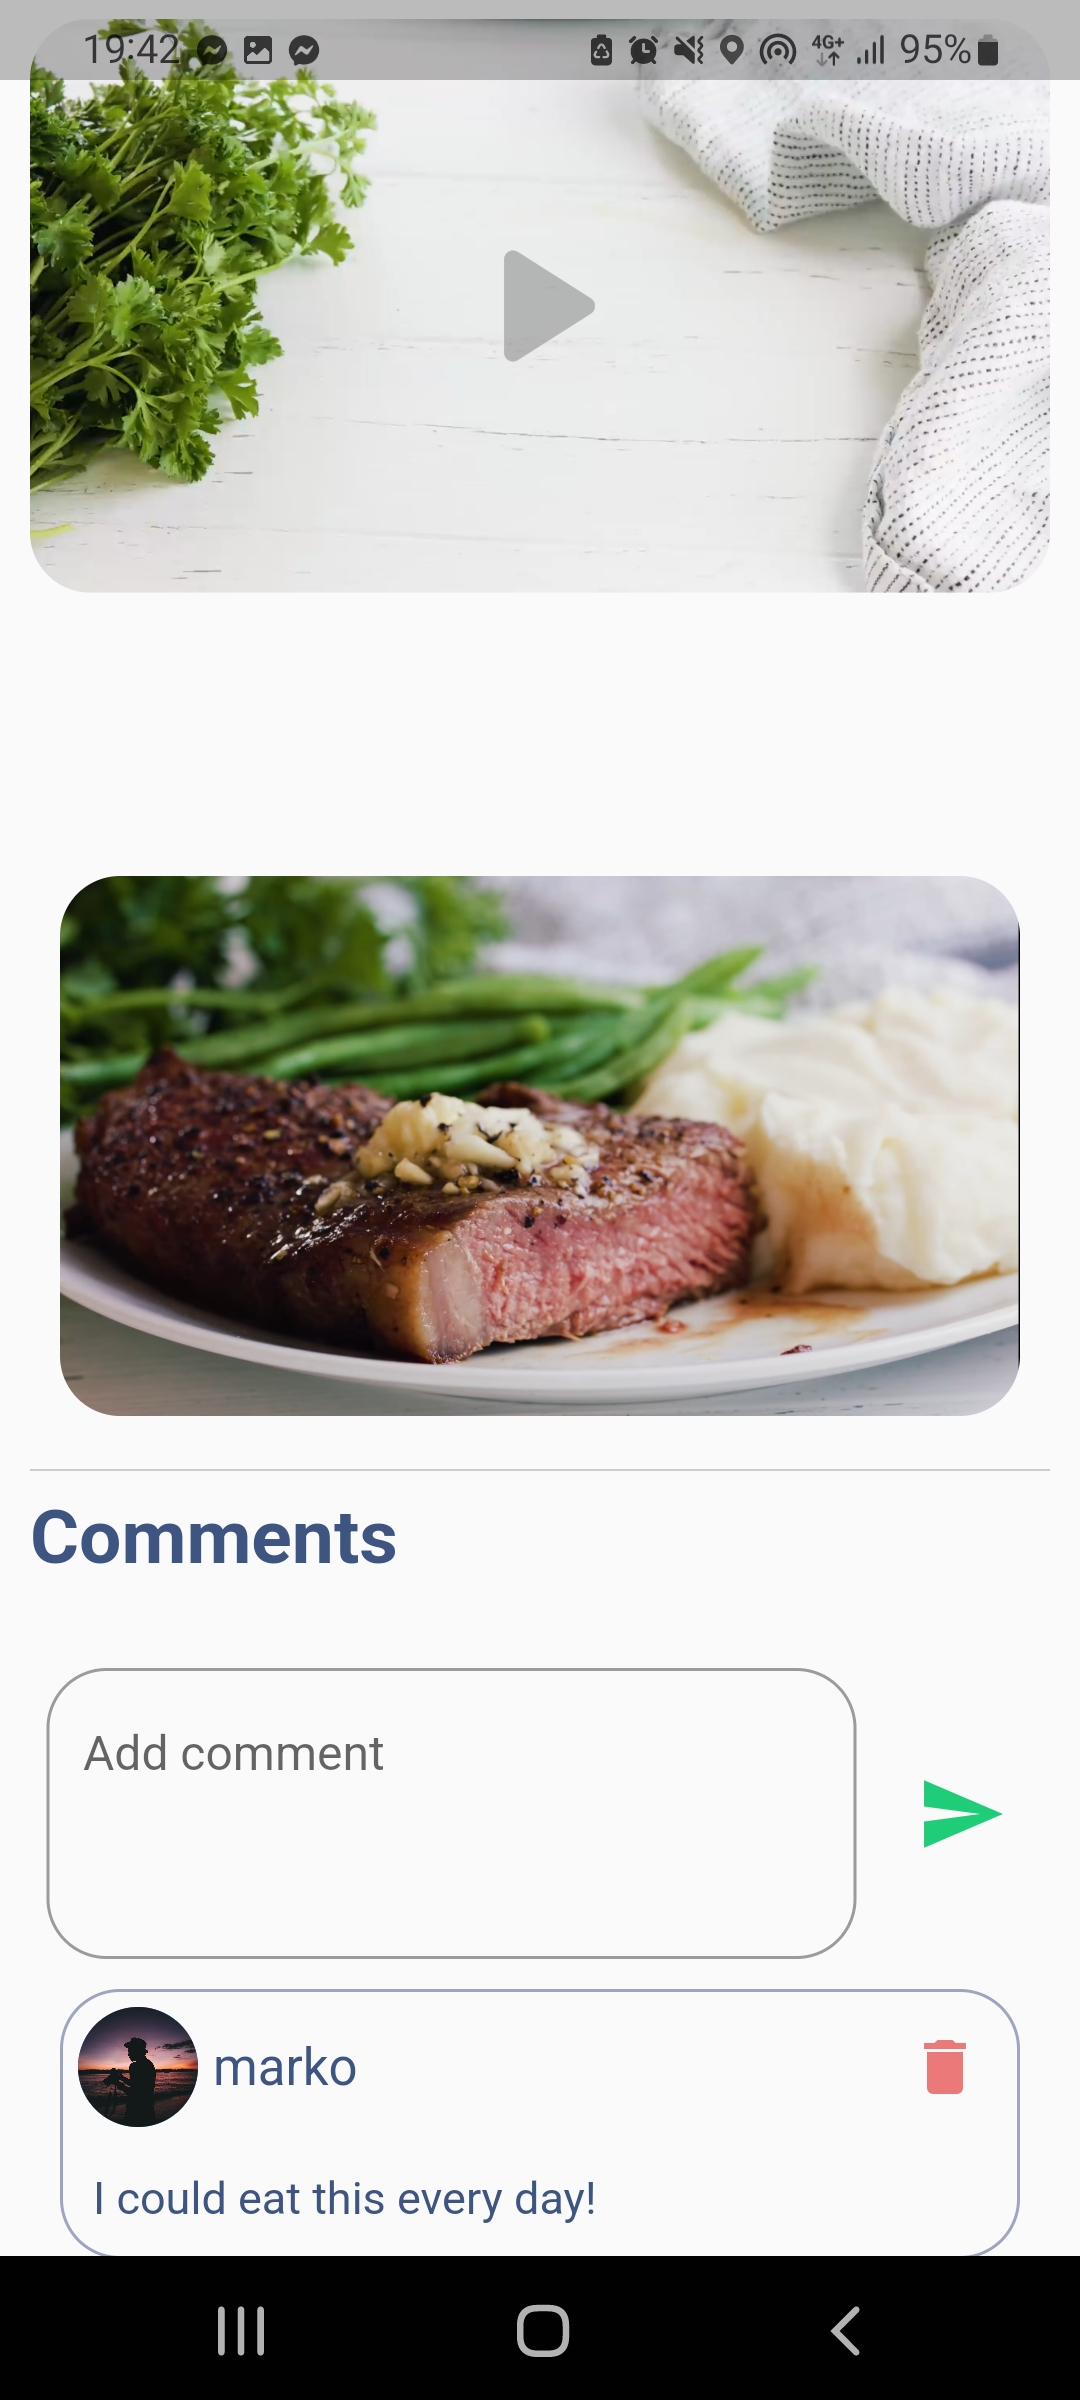
\includegraphics[width=.25\textwidth]{images_videos_comments.jpg} }}
      \caption{Ekran za dodavanje recepta i pregled recepta}
      \label{fig:New recipe}
\end{figure}\newpage
Na sljedećem ekranu nalaze se svi podaci o pojedinačnom receptu. Do tog se ekrana dolazi klikom na recept
sa četvrtog ekrana. Uz sve podatke o receptu mora postojati i prostor za ostavljanje komentara i ocjene (slika \ref*{fig:New recipe} (a) i (b)).
Kada
je administrator pristupio receptu mora postojati gumb za odobravanje odnosno poništavanje odobrenja recepta (slika \ref*{fig:Single recipe} (b)).
Da bi se omogućile navedene funkcionalnosti, mora se pristupati uslugama dohvaćanja odabranog recepta,
ostavljanju komentara, ocjenjivanja i odobravanja recepta na poslužitelju.\\
\begin{figure}[h]
      \centering
      \subfloat[\centering Ekran za upravljanje korisnicima]{{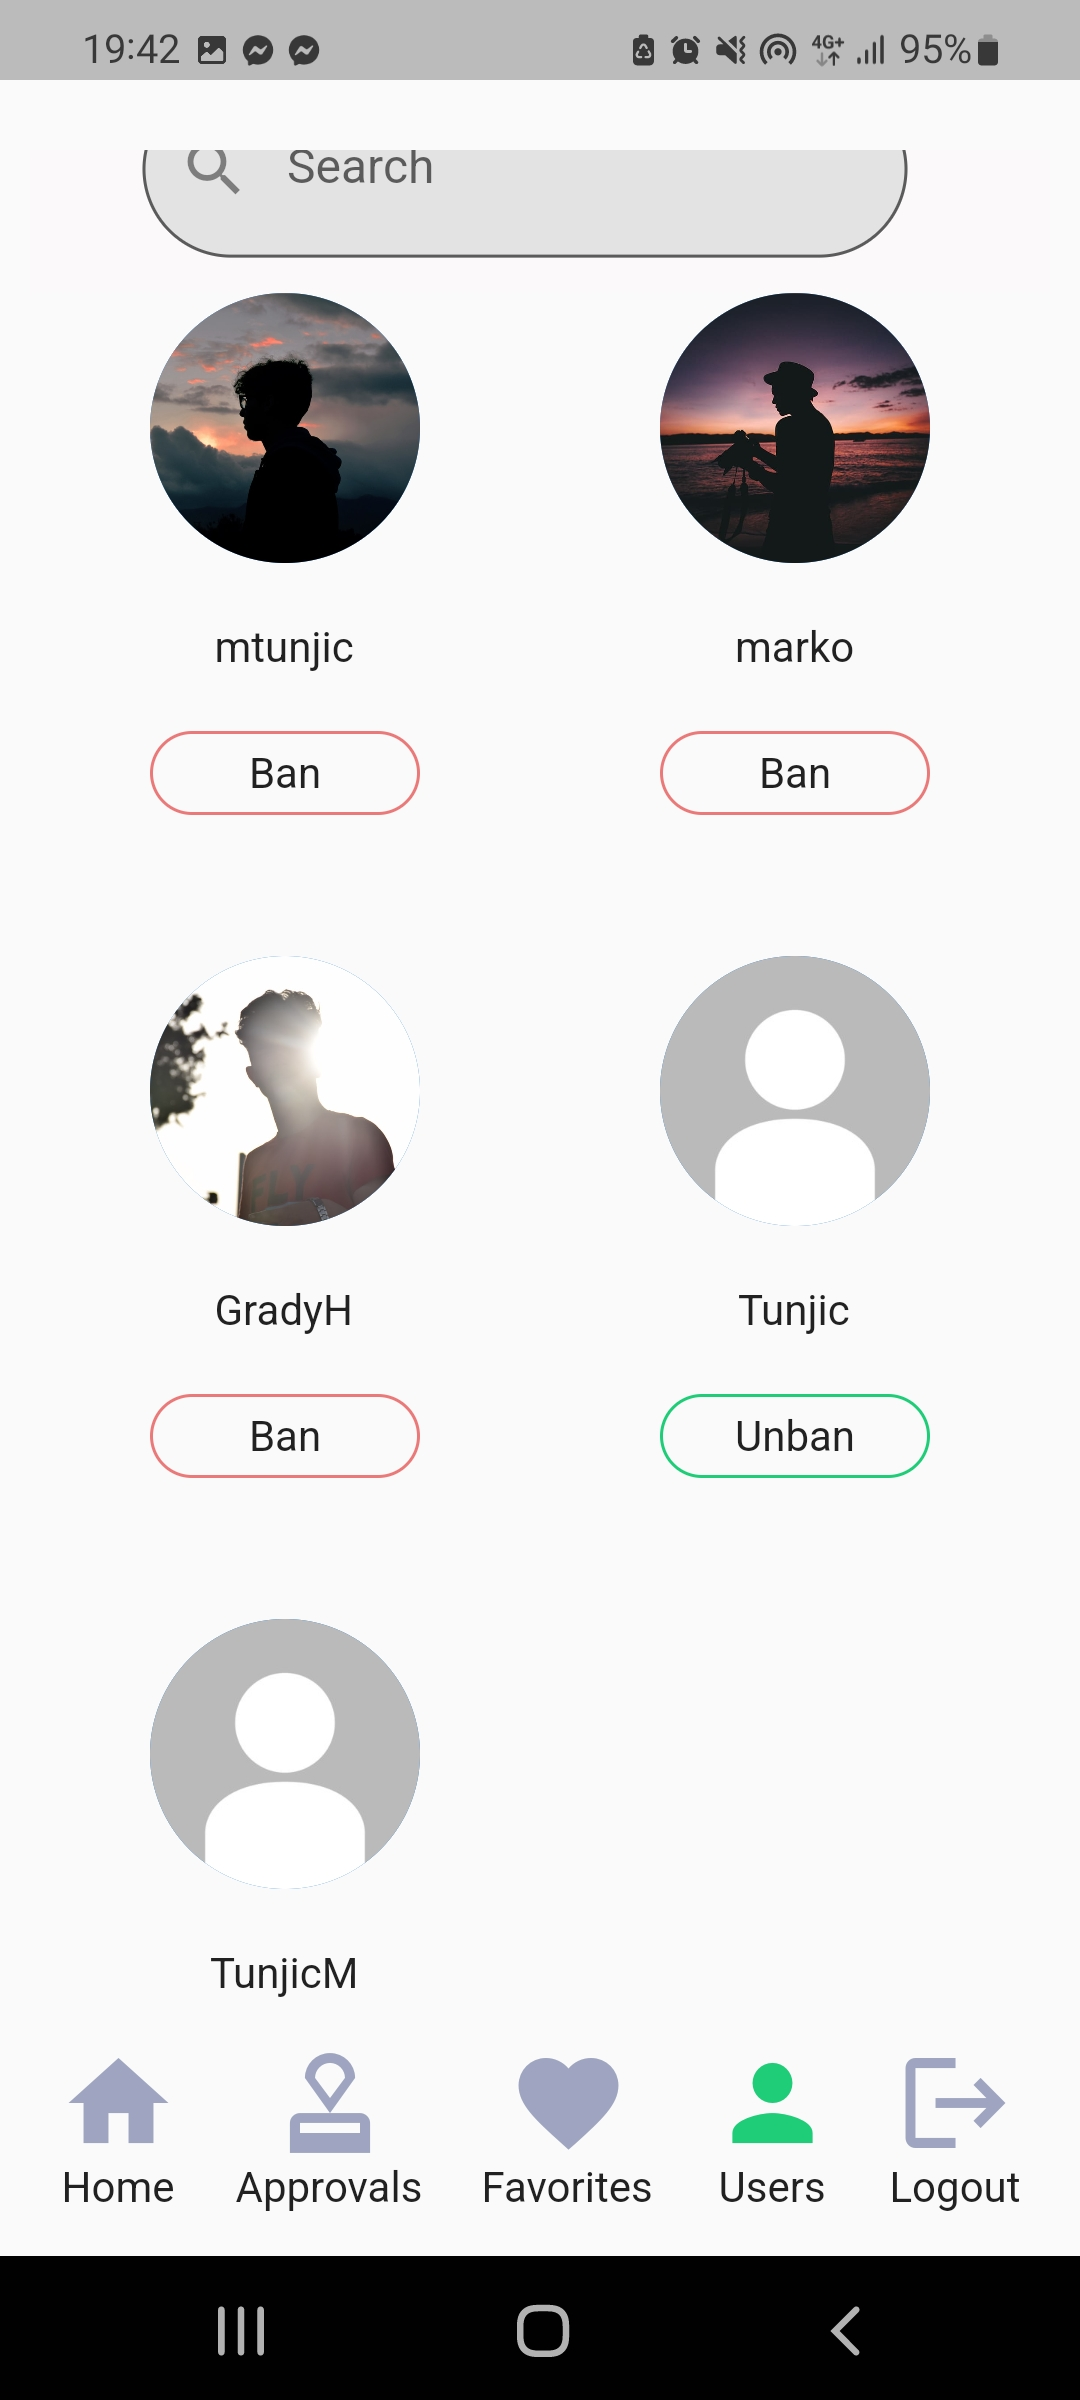
\includegraphics[width=.25\textwidth]{bans.jpg} }}
      \subfloat[\centering Ekran za odobravanje recepata]{{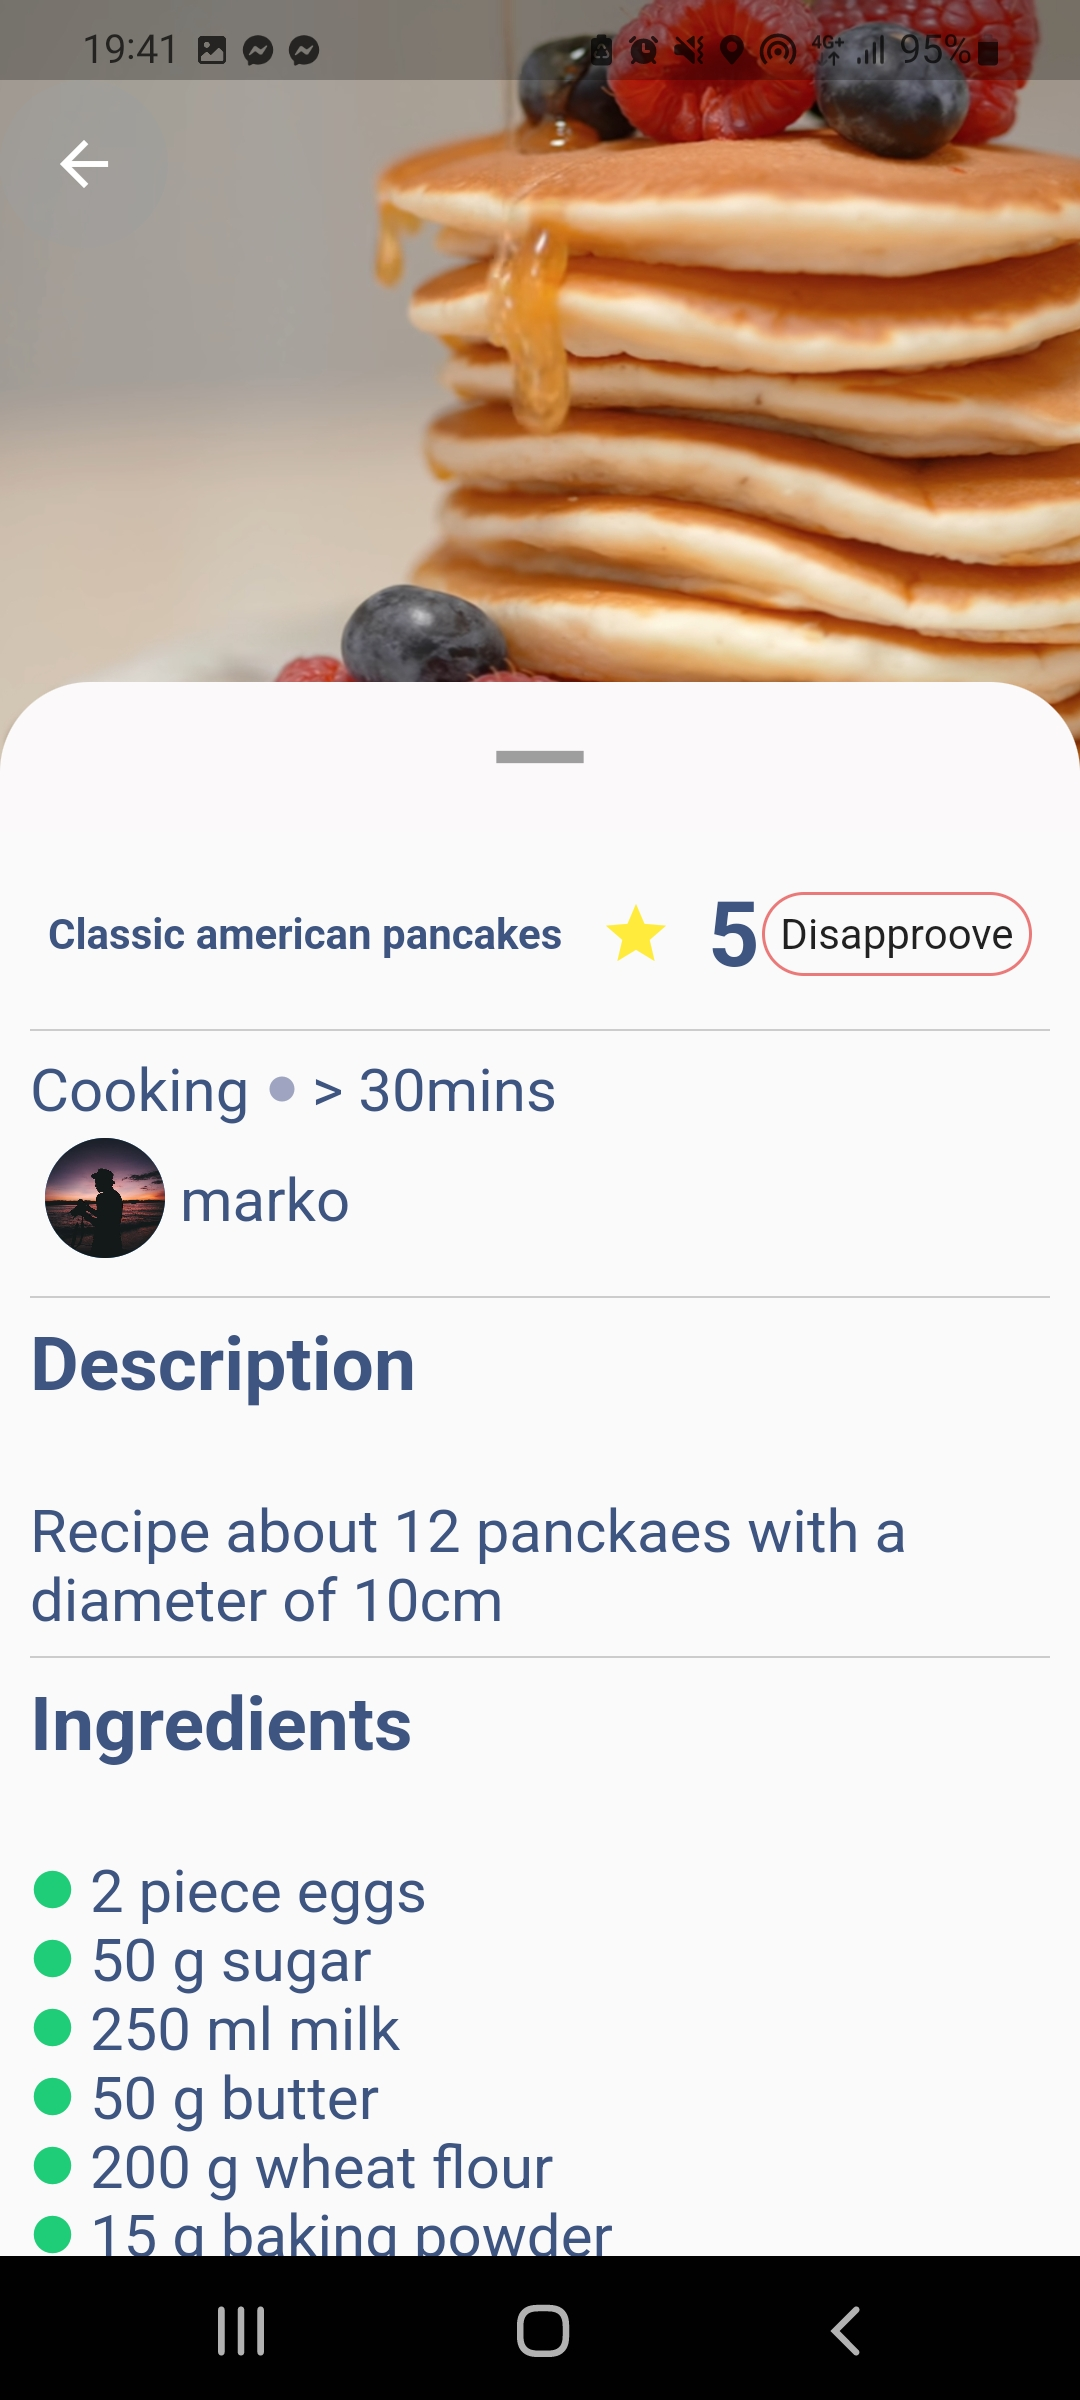
\includegraphics[width=.25\textwidth]{single_recipe_admin.jpg} }}
      \caption{Ekrani za administratore}
      \label{fig:Single recipe}
\end{figure}\newpage
Sedmi ekran je rezervian samo za administratore i na njemu se nalaze svi registrirani korisnici
i elementi koji će omogućiti slanje zahtjeva za suspendiranje korisnika (slika \ref*{fig:Single recipe} (a)).
Osmi i deveti ekrani su jednaki kao i četvrti ekran, razlikuju se samo u receptima koji su prikazani.
Na osmom ekranu moraju biti prikazani samo recepti koji se nalaze u favoritima za trenutno prijavljenog korisnika, a na devetom
samo neodobreni recepti (slika \ref{fig:special}).
To se postiže postavljem odgovarajućeg atributa u filter i slanjem zahtjeva na poslužitelj.
\begin{figure}[h]
      \centering
      \subfloat[\centering Ekran sa favoritima]{{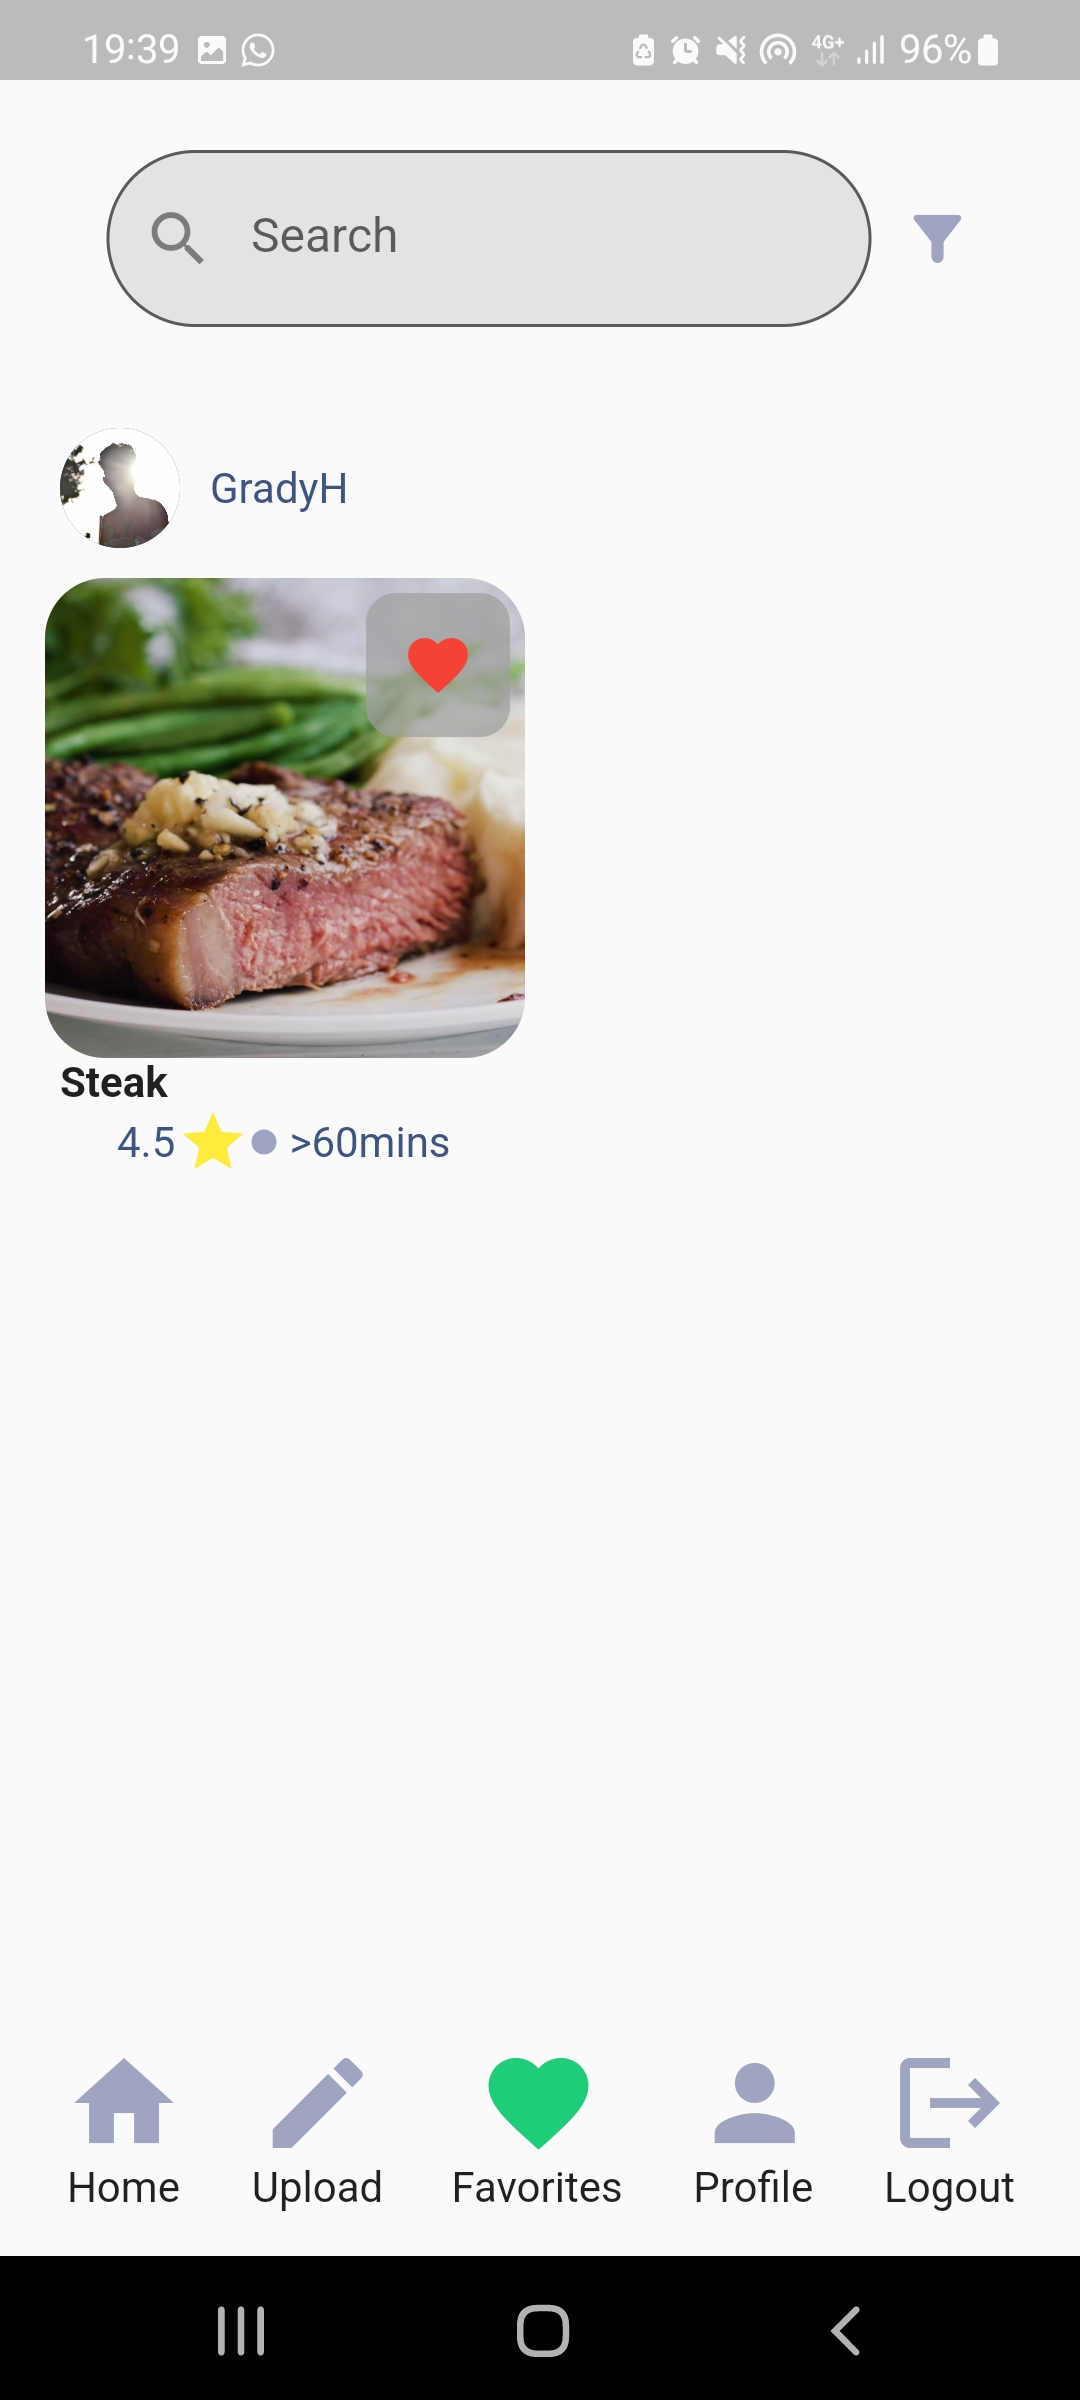
\includegraphics[width=.25\textwidth]{favorites.jpg} }}
      \subfloat[\centering Ekran sa neodobrenim receptima]{{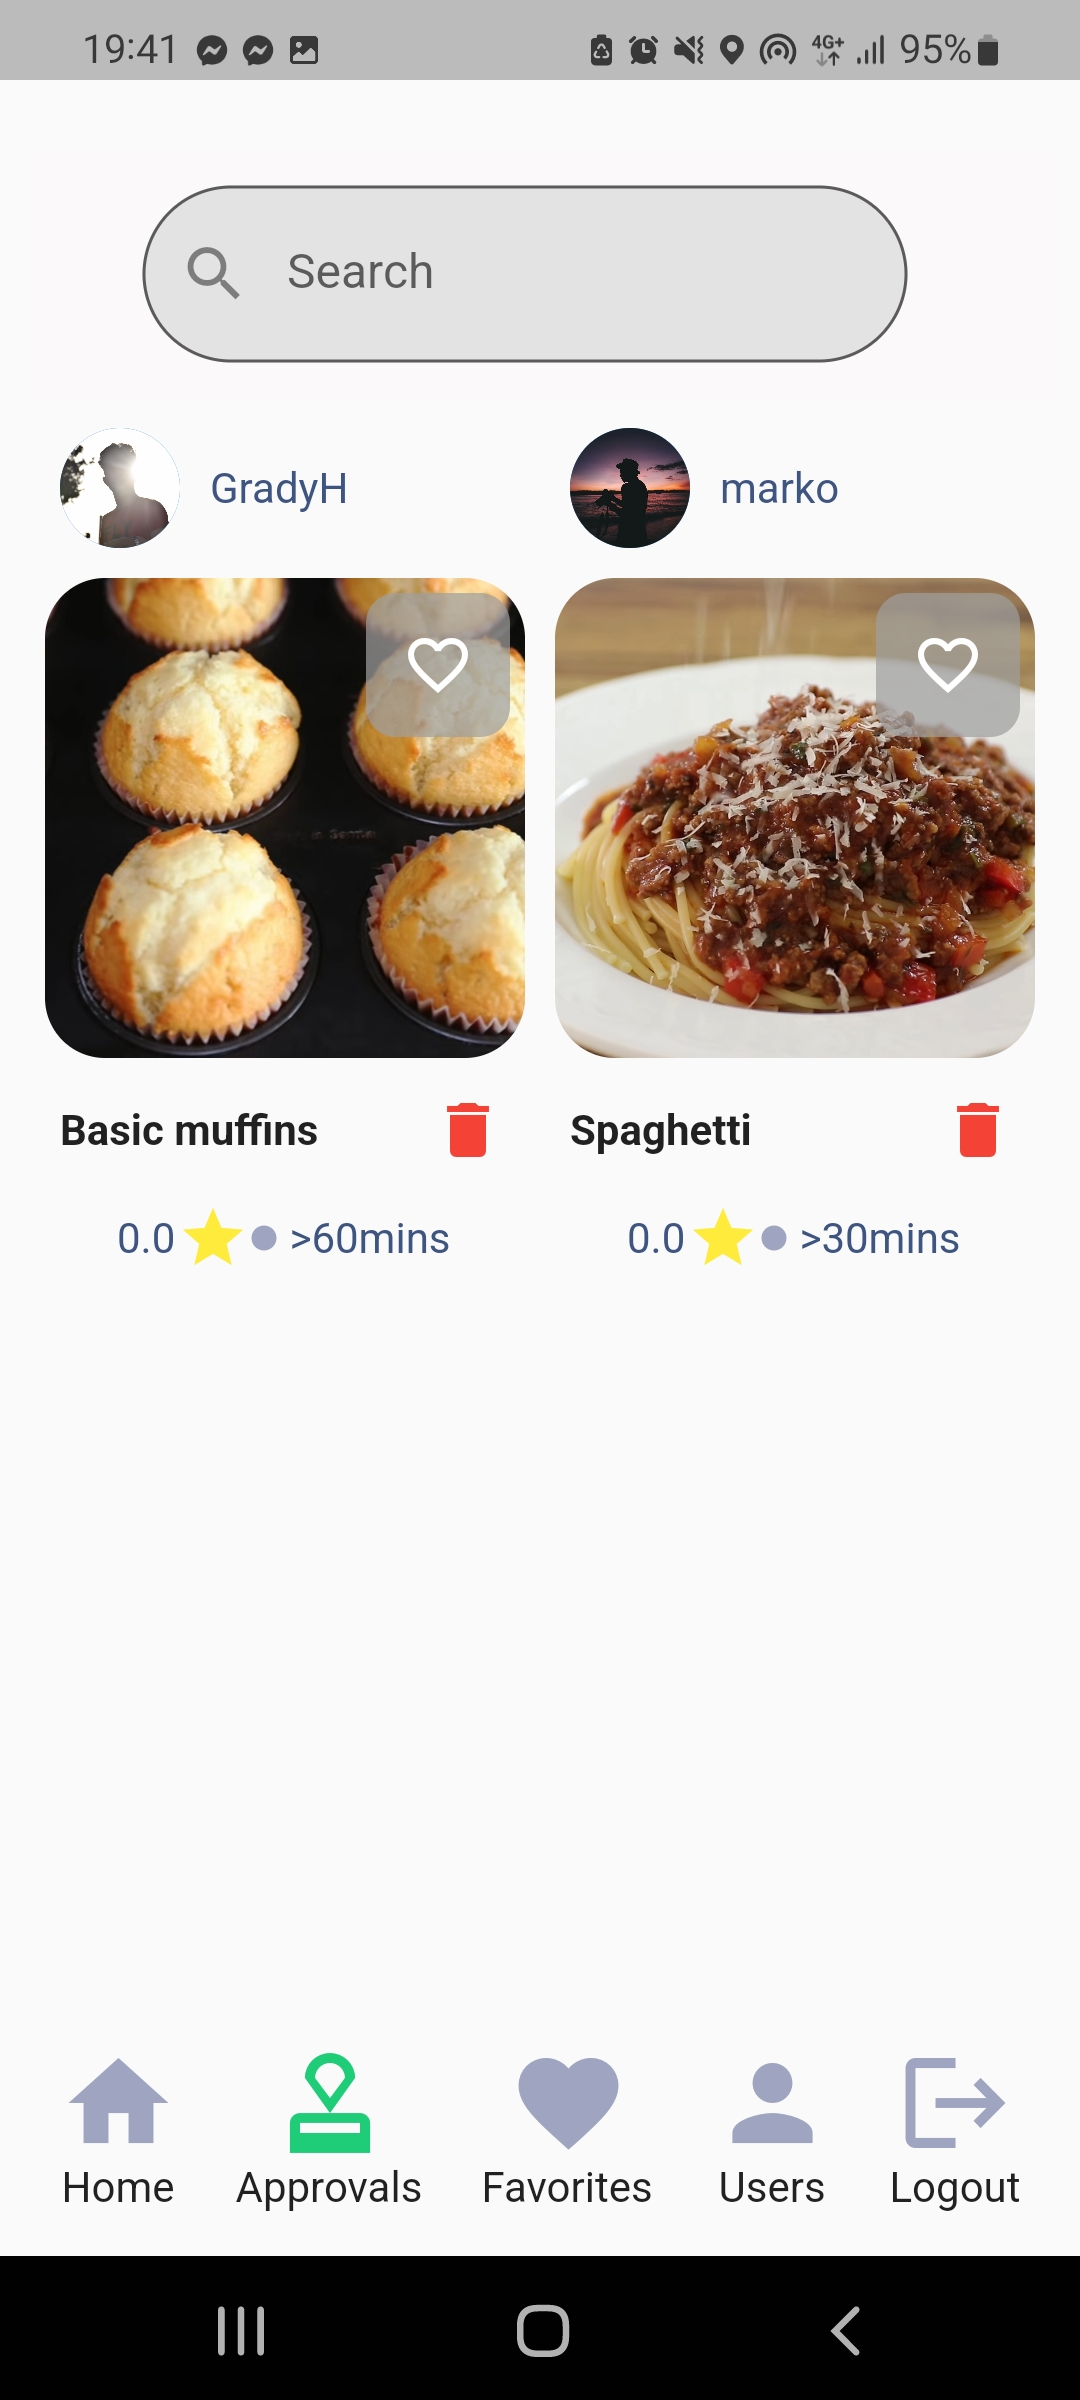
\includegraphics[width=.25\textwidth]{approovals.jpg} }}
      \caption{Ekran sa favoritima i ekran sa neodobrenim receptima}
      \label{fig:special}
\end{figure}\\


\chapter{Arhitektura}
U ovom poglavlju je opisana arhitektura, implementacija
i korištene tehnologije na poslužiteljskoj i korisničkoj strani aplikacije.
\section{Poslužiteljska strana}
Poslužiteljska strana pisana je u programskom jeziku Java (ref \cite{ProgramiranjeUJavi}) verzije 11 jer je najnovija podržana verzija
u odabranoj usluzi oblaka upravo Java 11. Korišteni radni okvir je
\textit{SpringBoot} (ref. \cite{GraphQL}) koji je namijenjen upravo za izradu poslužiteljske strane web i mobilnih aplikacija.
Kao arhitekturni stil korišten je GraphQL koji predstavlja upitni jezik koji je specifično dizajniran za korisničku stranu aplikacije.
Tako GraphQL omogućava korisničkoj strani da od poslužiteljske strane zatraži i dobije samo one podatke koji su potrebni.
Projekt je strukturiran kao Maven (ref. \cite{maven}) projekt koji omogućava dohvat i korištenje biblioteka koje nisu
dio standardnog javinog paketa.
Za verzioniranje projekta je korišten alat Git (ref. \cite{git}) koji nudi razne mogućnosti, ali jedna od
bitnijih je da je vrlo lako vratiti projekt na staru verziju
ukoliko se dogodi veća pogreška u pisanju programskog koda. Za upogonjavanje
se kao i za bazu podataku koristi \textit{AWS} (ref. \cite{AWS}), ali drugi servis: \textit{ElasticBeanstalk (ref. \cite{EB})} servis.
Navedeni servis omogućava da se samo uploada .jar arhiva i sve ostalo će biti
automatski dodano.
U svrhe razvoja korišteno je okruženje \textit{VSCode} (ref. \cite{vsc}).

\subsection{GraphQL}

\subsubsection{Povijest}
Jedan od većih problema dizajniranja web poslužitelja pa tako i samih web aplikacija u REST (ref. \cite{REST})
arhitekturnom stilu je problem prekomjernog dohvata podataka odnosno nedovoljnog dohvata podataka
\textit{(eng. overfetching and underfetching)}. Ako bi se taj problem pokušao riješiti sa REST
arhitekturnim stilom bilo bi potrebno stvariti više krajnjih točaka \textit{(eng. endpoint)} za dohvat specifičnog skupa podataka,
a uz to i više prijenosnih objekata.
Uloga takvih objekata je spremanje i slanje samo onih podataka koji su potrebni za ispunjavanje zahtjeva.
\\\\
Tako je tvrtka Facebook došla
do ideje GraphQL-a. Naime, razvojni programeri su tada radili s velikim brojem podataka koji su
bili međusobno ugnježđenji i povezani na razne načine. Da bi aplikacija radila dovoljno brzo
i efikasno bilo je nužno dohvatiti samo one podatke koji se uistinu i koriste, a da se pritom dohvaćaju koristeći
što manje zahtjeva.

\subsubsection{Definicija}
GraphQL je upitni jezik koji korisničkoj strani
dopušta definiranje formata i oblika podataka koji će zahtjevati od poslužiteljske strane. Također omogućava
da se upiti šalju na samo jednu krajnju točku. U GraphQL-u postoje 2 vrste upita:
upiti i mutacije \textit{(eng. query and mutation)}. Razlika je u tome što upiti služe za dohvaćanje podataka,
a mutacije za mijenjanje podataka.

\subsubsection{Implementacija}
U okviru ovoga rada u \textit{pom.xml} datoteku u kojoj se dodaju ovisnosti \textit{(eng. dependencies)}
bilo je potrebno dodati 2 nove ovisnosti: \textit{graphql-spring-boot-starter, graphql-java-tools}
i po potrebi treću ovisnost koja nudi mogućnost testiranja sučelja,
a ona je \textit{graphiql-spring-boot-starter} (odlomak \ref{graphqlDependecies}). Nakon toga ove ovisnosti zahtjevaju
izradu jedne datoteke u kojoj će pisati sve moguće vrste podataka koje se mogu tražiti, i sve
moguće upite koji se mogu primiti. Takva datoteka se najčešće imenuje \textit{schema.graphqls}.
U ovom radu podaci u shemi su bili ujedno i relacijski modeli iz baze podataka.
Postoje razni upiti, a bili su dodavani jedan po jedan ovisno o potrebi aplikacije (odlomak \ref{graphqlSchema}).
U odlomku koji prikazuje GraphQL upite (\ref{graphqlType})
postoji velik broj mutacija i upita, ali to ne mijenja činjenicu da postoji
samo jedna krajnja točka koja je u ovom slučaju \textit{/graphql}. Iz priloženog primjera jednog GraphQL tipa podatka u odlomku \ref{graphqlType}
moguće je primjetiti da je tip podatka upravo jedan od relacijskih modela iz baze podataka. Razlika je u tome da postoje neki dodatni podaci
koji rješavaju problem nedovoljnog dohvata podataka. Bitan detalj je da se imena i tipovi polja iz Java klase i tipa podatka iz
GraphQL sheme moraju podudarati jer se koristi refleksija za dohvat tih polja. Refleksija služi za dohvaćanje i pozivanje po imenu
metoda iz opisnika klase.
\newpage
\subsubsection{GraphQL ovisnosti}
\label{graphqlDependecies}
\begin{Verbatim}[fontsize=\scriptsize]
<dependency>
      <groupId>com.graphql-java</groupId>
      <artifactId>graphql-spring-boot-starter</artifactId>
      <version>5.0.2</version>
</dependency>
<dependency>
      <groupId>com.graphql-java</groupId>
      <artifactId>graphql-java-tools</artifactId>
      <version>5.2.4</version>
</dependency>
<dependency>
      <groupId>com.graphql-java</groupId>
      <artifactId>graphiql-spring-boot-starter</artifactId>
      <version>5.0.2</version>
</dependency>
\end{Verbatim}

\paragraph{GraphQL upiti}
\label{graphqlSchema}
\begin{Verbatim}[fontsize=\scriptsize]
schema{
      query: Query
      mutation: Mutation
}
type Query{
      recipes(filter: Filter!): Recipes!
      singleRecipe(recipeId: ID!): Recipe!
      userForId(userId: ID!): Users!
      users(filter: Filter!): UsersResponse!
      notApprovedRecipes(filter: Filter!): Recipes!
      favorites(userId: ID!, filter: Filter!): Recipes!
}
type Mutation{
      login(identifier: String!,password:String!): LoginResponse!
      register(payload: RegisterRequest!): Users!
      addRecipe(payload: RecipePayload!): Recipe!
      editFavorite(userId: ID!, recipeId: ID!, state: Boolean!): Boolean!
      deleteRecipe(recipeId: ID!): Boolean!
      addComment(userId: ID!,recipeId: ID!,commentText: String!): Comments
      addRating(userId: ID!,recipeId: ID!, ratingValue: Int!): Boolean!
      deleteComment(commentId: ID!): Boolean!
      changeBanStatus(userId: ID!, banStatus: Boolean!): Boolean!
      changeApproovedStatus(recipeId: ID!, isApprooved: Boolean!): Boolean!
}
\end{Verbatim}
\paragraph{GraphQL tip podatka}
\label{graphqlType}
\begin{Verbatim}[fontsize=\scriptsize]
type Recipe{
      id: ID!
      coverPicture: String!
      recipeName: String!
      description: String!
      isApprooved: Boolean!
      cookingDuration: Int!
      user: Users!
      recipeSteps: [RecipeStep] @relation
      ingredients: [Ingredient] @relation
      images: [Image] @relation
      videos: [Video] @relation
      ratings: [Rating] @relation
      comments: [Comments] @relation
      favoriteTo: [Favorite] @relation
      averageRating: Float
      isLikedByCurrentUser: Boolean
      ratingFromCurrentUser: Int!
}
\end{Verbatim}
Nakon dodavanja sheme i ovisnosti potrebno je dodati razrješivače (eng. \textit{resolvere}). U ovom projektu postoje 3 vrste razrješivača:
\textit{QueryResolver, MutationResolver} i obični \textit{Resolver}, oni su u prethodno navedenim ovisnostima definirani kao sučelja:
\textit{GraphQLQueryResolver}, \textit{GraphQLMutationResolver}, \textit{GraphQLResolver}. Prvi služi za prihvaćanje upita, drugi za prihvaćanje
mutacija, a treći služi za rješavanje problema prethodno spomenutih dodatnih parametara koji su umetnuti u GraphQL shemu. To se radi
na način da se zasebno definira način dohvata tih podataka. Također se može implementirati sučelje GraphQLErrorHandler koji
će presretati greške s poslužiteljske strane i vraćati odgovarajuću poruku korisničkoj strani. Naime, GraphQL
ima jednu manu, a to je da se na korisničku stranu uvijek vraća HTTP status kod 200 OK, pa se rukovanje greškama
obavlja na drukčiji način - u slučaju greške u odgovor se doda parametar \textit{errors} koji će sadržavati
sve greške koje su se dogodile (slika \ref{fig:Handled error}).
Ako se ne implementira sučelje \textit{GraphQLErrorHandler} poslužitelj će uvijek vraćati predefiniranu pogrešku. \\
\begin{figure}[h]
      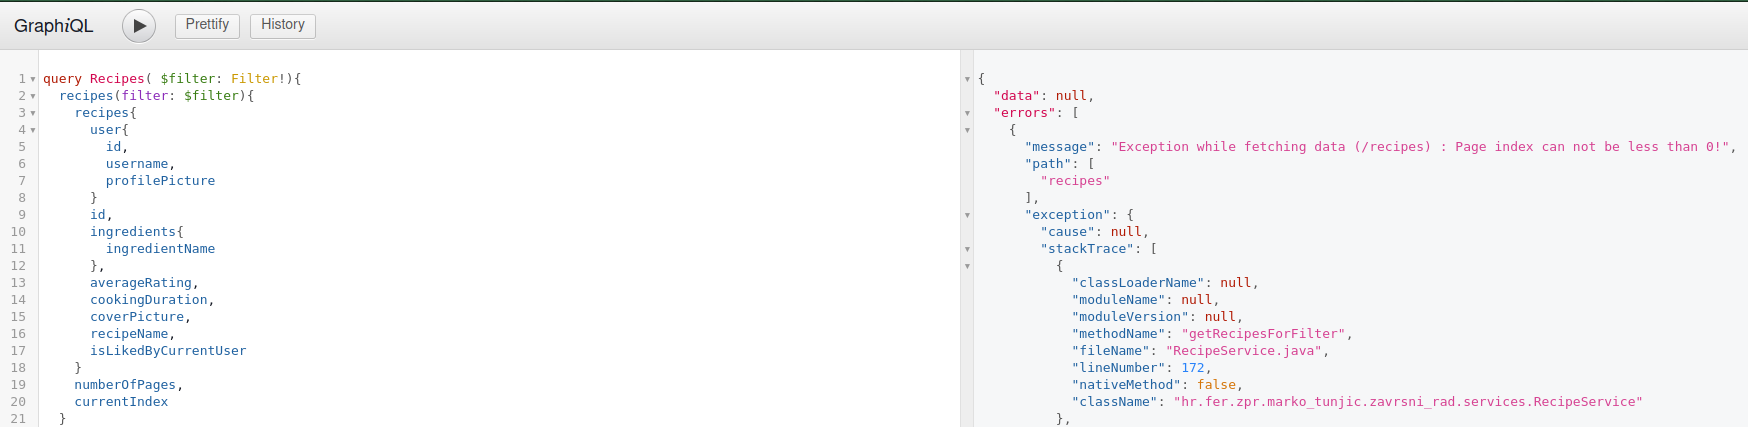
\includegraphics[width=\textwidth]{graphql_handled_error.png}
      \caption{Primjer greške ako postoji GraphQLErrorHandler}
      \label{fig:Handled error}
\end{figure}
\\
Nakon implementacije svih navedenih sučelja (slika \ref{fig:GraphQL implementation}) se
uspješno može izvršiti prvi upit koji je demonstriran kroz sučelje \textit{GraphiQL} i
prikazuje strukturu upita i odgovora (slika \ref{fig:GraphQL query}).
\begin{figure}[h]
      \centering
      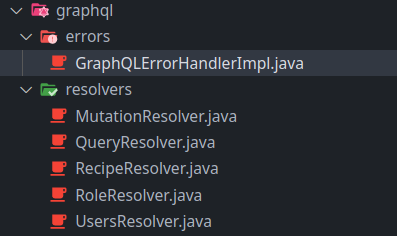
\includegraphics[width=.5\textwidth]{graphql_implementation_classes.png}
      \caption{Struktura GraphQL paketa}
      \label{fig:GraphQL implementation}
\end{figure}
\begin{figure}[h]
      \centering
      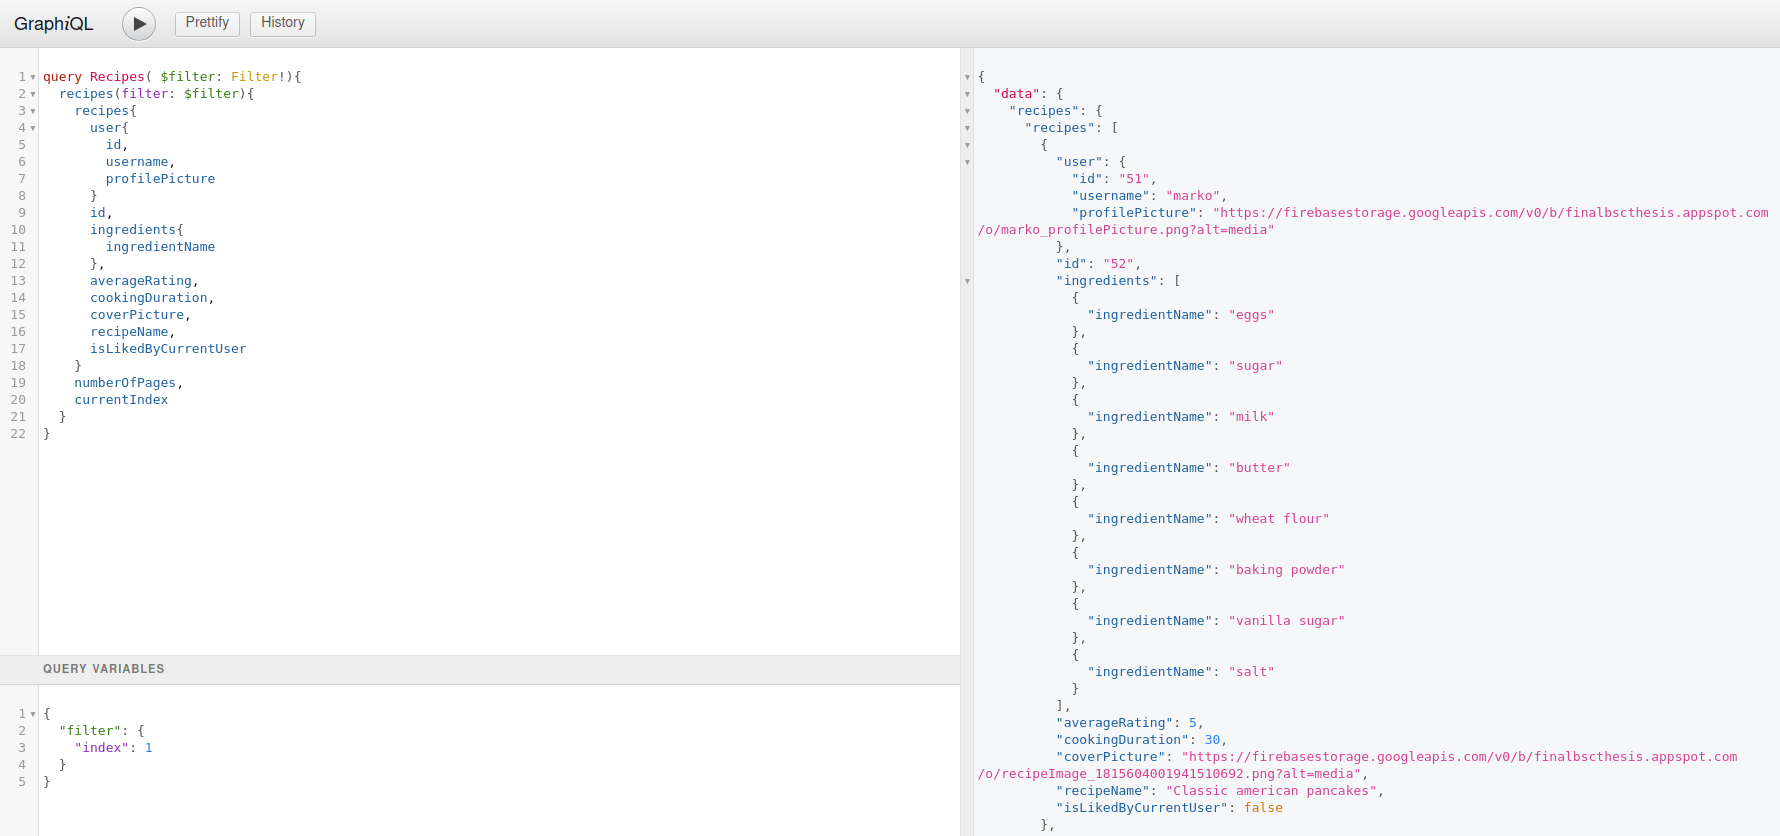
\includegraphics[width=\textwidth]{graphql_query.png}
      \caption{Primjer ispravnog upita}
      \label{fig:GraphQL query}
\end{figure}


\subsection{Autentifikacija i autorizacija}

\subsubsection{JWT}
U području autentifikacije i autorizacije vidi se jedna velika razlika između
moderne izrade mobilne i web aplikcije, a to je odsutnost sesije odnosno nacina očuvanja stanja izmešu klijenta i poslužitelja. Jedna od namjena sesije je
identificiranje trenutno prijavljenog korisnika na temelju nekog atributa koji je jedinstven za tog korisnika.
Problem kod implementacije sesija je uporaba kolačića koji se ne koriste u mobilnim aplikacijama.
Zato se mobilne aplikacije koriste drugim mehanizmom, a
to su tokeni. U ovoj aplikaciji se koriste tokeni pod imenom \textit{JWT (JSON Web Token)} (ref. \cite{jwt}), koji
u sebi sadrže podatke koji se koriste za uspostavu autentifikacije korisnika. Da bi se ti podaci
mogli sigurno prenositi između poslužiteljske i korisničke strane koriste se
kriptografski algoritmi (kao na primjer HMACSHA256 (ref. \cite{HMAC})) za enkripciju tokena.
U nekom takvom tokenu će se primjerice nalaziti nalaziti korisničko ime, istek tokena, korišteni algoritmi i slični podaci koji će omogućiti
autentifikaciju i autorizaciju korisnika aplikacije.

\subsubsection{Autentifikacija}
Da bi se ovo ostvarilo prvo je bilo potrebno dodati ovisnost prema \linebreak
\textit{SpringSecurity-u} i prema \textit{JJWT-u} (odlomak \ref{Security dependency}). Nakon toga, da bi aplikacija mogla doći do podataka trebalo je implementirati dva sučelja
\textit{UserDetails} i \textit{UserDetailsService}. Prvo sučelje služi za omotavanje osnovnih podataka o korisniku,
kao na primjer korisničko ime, lozinka, je li korisnik suspendiran, je li korisnik potvrdio svoj identitet,
koje su korisnikove uloge (administrator ili korisnik) i slično.
Drugo sučelje služi za dohvat tih podataka na osnovu korisničkog imena jer je to jedinstven atribut za svakog korisnika.
U ovoj aplikaciji sučelje \textit{UserDetails} omotava
podatke iz baze podataka, a sučelje \textit{UserDetailsService} dohvaća podatke iz baze i sprema ih u prvo sučelje.
\paragraph{Ovisnosti prema bibliotekama potrebnih za implementaciju autentifikacije i autorizacije}
\label{Security dependency}
\begin{Verbatim}[fontsize=\scriptsize]
<dependency>
      <groupId>org.springframework.boot</groupId>
      <artifactId>spring-boot-starter-security</artifactId>
</dependency>
<dependency>
      <groupId>io.jsonwebtoken</groupId>
      <artifactId>jjwt</artifactId>
      <version>0.9.1</version>
</dependency>
\end{Verbatim}
Nadalje, kako bi se ti podaci mogli dohvatiti u bilo kojem trenutku potrebno ih je u nekom trenutku spremiti.
Zato je bilo potrebno napraviti jedan \textit{Filter}. \textit{Filteri} su posebni objekti u web aplikaciji koji presreću bilo koji
zahtjev koji stigne na poslužitelj, obrade taj zahtjev i proslijede ga dalje prema web aplikaciji.
Filter za autentifikaciju će provjeriti postoji li HTTP zaglavlje \textit{Authorization} i, ako
postoji, pretpostavit će da se unutra nalazi token kojeg će pokušati analizirati i iz njega dohvatiti korisničko ime.
Na osnovu tog korisničkog imena i uz pomoć sučelja \textit{UserDetailsService} vrlo jednostavno se dohvati sučelje \textit{UserDetails}.
Da bi podaci bili dostupni cijelom poslužiteljskom dijelu aplikacije, filter će spremiti bitne podatke u klasu koja se zove
\textit{SecurityContextHolder} koja će pružiti mogućnost dohvata trenutnog
korisnika u bilo kojem trenutku.
\\\\
Jedan od mogućih scenarija je da će token biti ili nevažeći ili isteknut zato je potrebno napraviti
ulaznu točku koja će (eng. \textit{EntryPoint}) u slučaju pogrešne autorizacije korisniku vratiti odgovarajuću poruku. Ta
ulazna točka
se u implementaciji naziva \textit{AuthenticationEntryPoint} koja putem HTTP odgovora šalje pogrešku u svojoj metodi commence. Struktura
svih implementiranih sučelja u projektu prikazana je na slici \ref{fig:Security}

\begin{figure}[h]
      \centering
      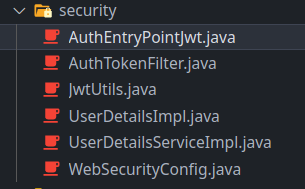
\includegraphics[width=.5\textwidth]{security_implementation.png}
      \caption{Struktura paketa za autentifikaciju i autorizaciju}
      \label{fig:Security}
\end{figure}

\subsubsection{Autorizacija}
Na kraju je potrebno definirati autorizaciju i spojiti s autentifikacijom, a to se obavlja tako da se
proširi klasa \textit{WebSecurityConfigurerAdapter}.
U njoj je definirano koja će se ulazna točka koristiti u slučaju pogreške, koji algoritam se koristi za šifriranje lozinki,
kada se poziva filter za autentifikaciju i kada se obavlja autorizacija. U ovoj aplikaciji se koristi prethodno
definirana ulazna točka, za šifriranje lozinke se koristi \textit{BCrypt} (ref. \cite{BCrypt}) algoritam, filter se poziva prije svakog zahtjeva, a
autorizacija se definira za svaku metodu zasebno. To se obavlja
uz pomoć oznake \textit{@PreAuthorize} (slika \ref{fig:WebSecurityConfig}).
Ona se koristi na način da se u tijelo oznake stave sve uloge koje smiju pristupati označenoj metodi (slika \ref{fig:PreAuthorize}).
One se najčešće stavljaju ili u \textit{QueryResolver-u} ili u \textit{MutationResolver-u} i tako će se ograničiti pristup
neautoriziranim korisnicima.
\begin{figure}[h]
      \centering
      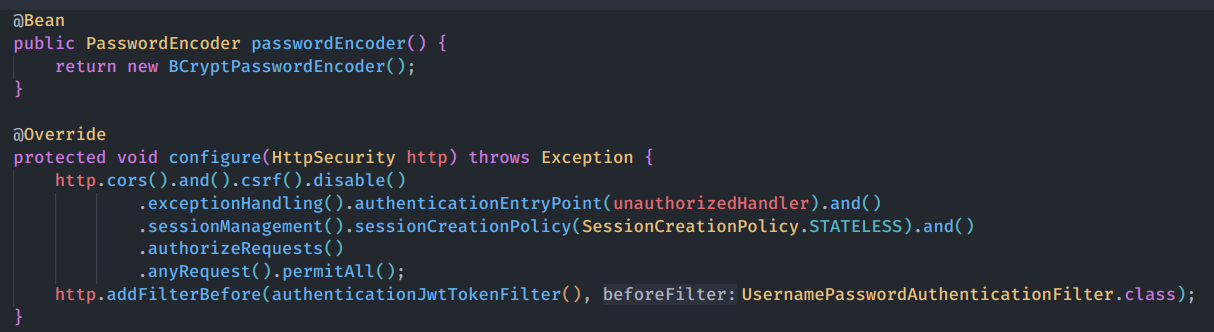
\includegraphics[width=\textwidth]{WebSecurityConfig.png}
      \caption{Izgled sigurnosne konfiguracije}
      \label{fig:WebSecurityConfig}
\end{figure}
\begin{figure}[h]
      \centering
      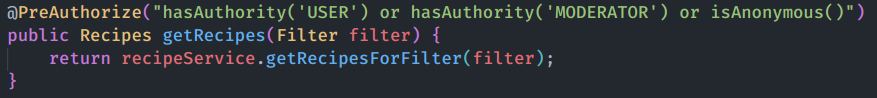
\includegraphics[width=\textwidth]{PreAuthorize.png}
      \caption{Izgled metode s oznakom @PreAuthorize}
      \label{fig:PreAuthorize}
\end{figure}
\newpage
\subsection{Pristup podacima}
Za pristup podacima se koriste dva sloja: prvi sloj je sloj za perzistenciju, a drugi je sloj usluge. Sloj za perzistenciju
modeliran je uz pomoć \textit{ORM-a (Object Realtional Mapper)} čija je zadaća preslikavanje relacija
iz baze podataka u Java objekte. Postoji više vrsta različitih ORM-ova, a u ovom projektu se koristi \textit{Hibernate} (ref. \cite{Hibernate}).
\\\\
U sloju usluge nalazi se sva logika potrebna za pristup i obradu podatka.
Sloj usluge je implementiran zbog razdvajanja odgovornosti obrade podataka i dohvata podataka od odgovornosti obrade zahtjeva.
Za sve to je bilo potrebno dodati ovisnost prema odgovarajućim
\textit{JPA} i \textit{JDBC} ovisnostima (odlomak \ref{dataAccess}).
\begin{figure}[h]
      \centering
      \subfloat[\centering Sve usluge]{{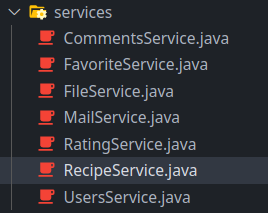
\includegraphics[width=.45\textwidth]{services.png} }}
      \caption{Izgled paketa za sloj usluge}
      \label{fig:services}
\end{figure}
\paragraph{Ovisnosti potrebne za pristupanje podacima}
\label{dataAccess}
\begin{Verbatim}[fontsize=\scriptsize]
<dependency>
      <groupId>org.springframework.boot</groupId>
      <artifactId>spring-boot-starter-data-jdbc</artifactId>
</dependency>
<dependency>
      <groupId>org.springframework.boot</groupId>
      <artifactId>spring-boot-starter-data-jpa</artifactId>
</dependency>
<dependency>
      <groupId>org.springframework.boot</groupId>
      <artifactId>spring-boot-starter-mail</artifactId>
</dependency>
<dependency>
      <groupId>com.google.firebase</groupId>
      <artifactId>firebase-admin</artifactId>
      <version>7.0.1</version>
</dependency>
\end{Verbatim}


\subsubsection{Sloj za perzistenciju}
U programskom jeziku Java, \textit{hibernate} se koristi kroz \textit{JPA} (Java Persistence API) programsko sučelje.
\textit{JPA} zahtjeva da se način preslikavanja iz relacije u objekt definira ili oznakama
ili u posebnoj konfiguracijskoj datoteci. U ovom projektu je to učinjeno preko anotacija, a sve takve klase prikazane su na
slici \ref{fig:JPA} (a). Anotacije i način anotiranja koji se mora poštivati prikazan je na slici \ref{fig:JPA} (b).
U izvornom kodu implementacije vidljivo je
da u modelima ovoga projekta nisu označene sve veze koje su određene samom bazom podataka
jer je to riješeno uz pomoć razrješivača iz \textit{GraphQL-a}. Nakon kreiranja svih modela potrebno je napraviti sučelja koja nasljeđuju sučelje
\textit{JPARepository} preko kojeg se pristupa samim podacima, a u tom sučelju su definirane metode
za dohvaćanje svih relacija, metoda za dohvaćanje relacija po identifikacijskom (ili nekom drugom) atributu
i slične.
\begin{figure}[h]
      \centering
      \subfloat[\centering Primjer anotiranja klase]{{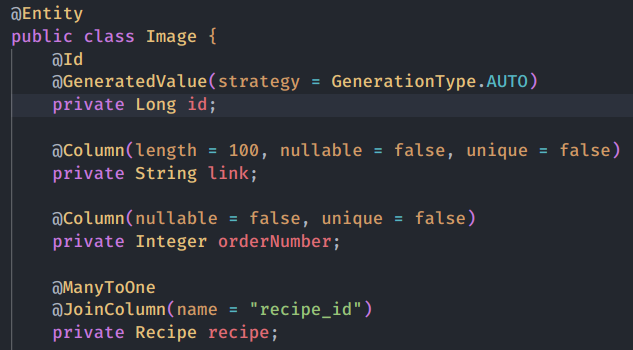
\includegraphics[width=\textwidth]{jpa_annotations.png} }}
      \caption{JPA konfiguracija}
      \label{fig:JPA}
\end{figure}
Također iz slike \ref{fig:JPA} (b)
na kojoj je prikazan model koji preslikava tablicu \textit{image} u Javinu klasu,
može se primjetiti da se slika u bazu sprema kao hiperveza na samu sliku. To je moguće jer se za
spremanje slika koristi \textit{Firebase} (ref. \cite{Firebase}). Firebase
je također jedna usluga u "oblaku" i u ovom radu se koristi za
spremanje datoteka. Za pristup firebase-u je bilo potrebno dodati ovisnost (odlomak \ref{dataAccess}) i jednu datoteku u kojoj su zapisani
podaci za pristup bazi koja iz sigurnosnih razloga nije priložena. Nakon je toga se primljena slika uz pomoć metode \textit{create}
prenosi na \textit{firebase oblak}.
\newpage
\subsubsection{Sloj usluge}
\label{serviceLayer}
Jedno od dobrih načela programiranja nalaže da jedna klasa ima samo jednu odgovornost
zato je sloj za perzistenciju od razrješivača odvojen slojem usluge.
\\\\
Također, osim same obrade podataka u sloju usluge nalazi se i klasa koja služi za slanje elektroničke pošte.
Ta usluga se koristi za slanje poruka za potvrdu identiteta i za slanje popisa za kupnju
koja se šalje ako neki korisnik doda recept u svoje favorite. Tijelo poruke se gradi
kao HTML dokument, a šalje se uz pomoć \textit{Java Mail API-a} za koji je bilo potrebno dodati ovisnost
prikazanu u odlomku \ref{dataAccess}. Konačno sve usluge prikazane su u odlomku \ref{dataAccess} (b).
Prikaz svih paketa (slojeva) i veza između njih nalazi se na slici (\ref{fig:packageDijagram})
\begin{figure}[h]
      \centering
      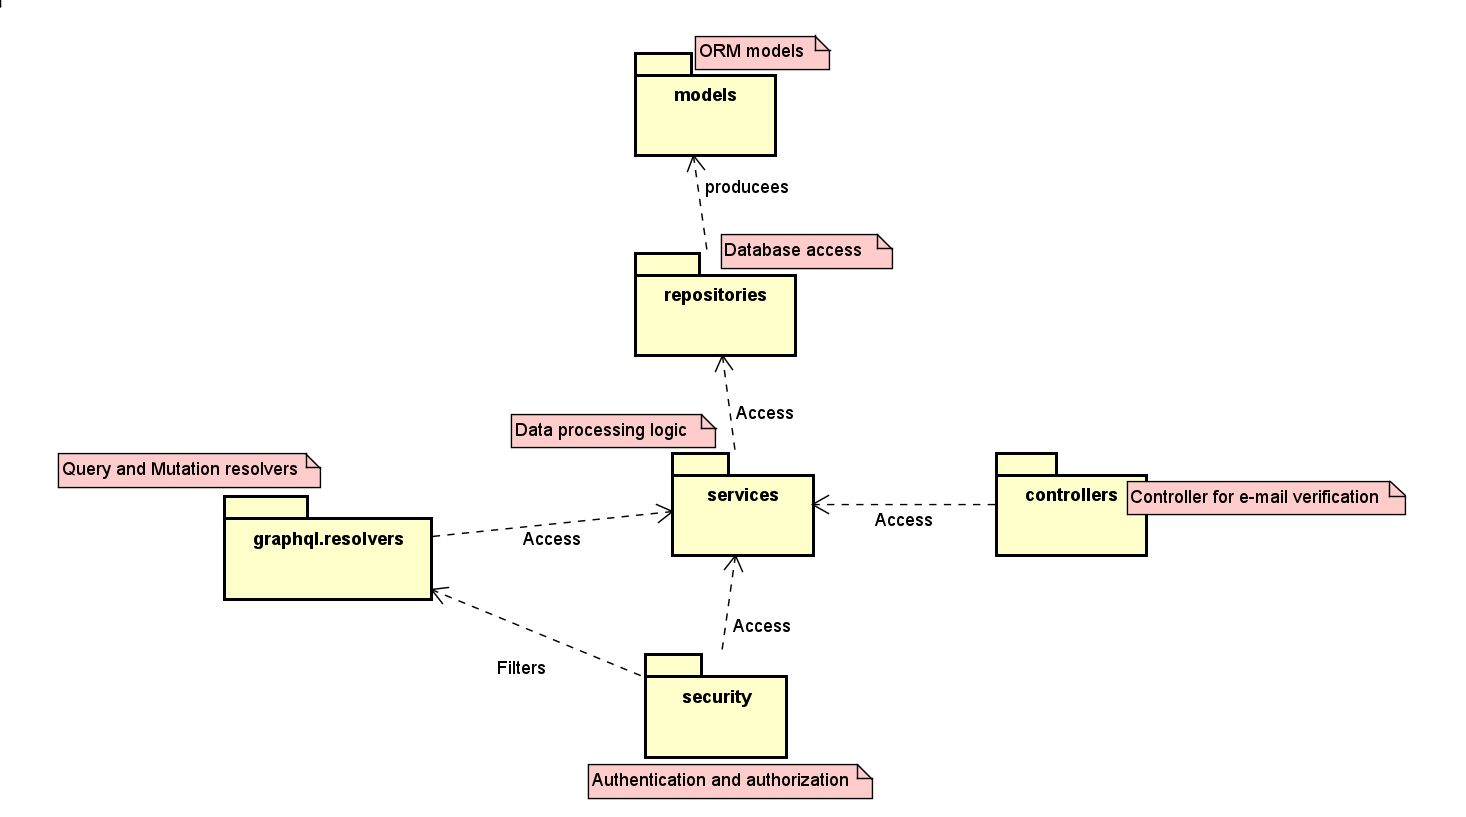
\includegraphics[width=\textwidth]{packageDiagram.png}
      \caption{Dijagram paketa}
      \label{fig:packageDijagram}
\end{figure}
\subsection{Kontinuirana isporuka}
Kontinuirana isporuka predstavlja proces prevođenja programskog koda i upogonjavanja na predviđeno mjesto (u ovom slučaju je to "oblak").
Ona se obavlja uz pomoć tzv \textit{Github} akcija. Jedna akcija je jedan pogramski kod
(slika \ref{fig:Backend cicd}) uz pomoć kojeg se izvorni kod prevodi u .jar arhivu i podiže na
oblak u \textit{AWS ElasticBeanstalk} servis.
Jedini problem je bio što nakon upogonjavanja poslužitelj može primati relativno male zahtjeve,
a za ovu aplikaciju su potrebni poprilično veliki zahtjevi jer se šalju i fotografije i videozapisi.
Fotografije i videozapisi se šalju sa korisničke na poslužiteljsku stranu pa tek onda
na \textit{firebase} iz sigurnosnih razloga. Naime, krajnji korisnici koji imaju loše namjere
mogu poslati maliciozne datoteke umjesto pretpostavljenih slika
i videozapisa pa je prije prihvaćanja datoteke potrebno provjeriti radi li se zaista o slici. Ova funkcionalnost
nije implementirana u ovom radu jer postoji mogućnost odobravanja recepta, ali unatoč tome to nije potpuno riješen problem.
Dakle, da bi se omogućilo slanje fotografija i videozapisa potrebno je
uz .jar arhivu  dodati i konfiguracijsku datoteku za \textit{ngnix} poslužitelj koja će povećati
pretpostavljenu maksimalnu veličinu zahtjeva. To je postignuto uz pomoć maven \textit{"antrun"} modula
(slika \ref{fig:antrun}) koji će .jar arhivu i konfiguracijsku datoteku spremiti u .zip arhivu i proslijediti dalje.
\begin{figure}[h]
      \centering
      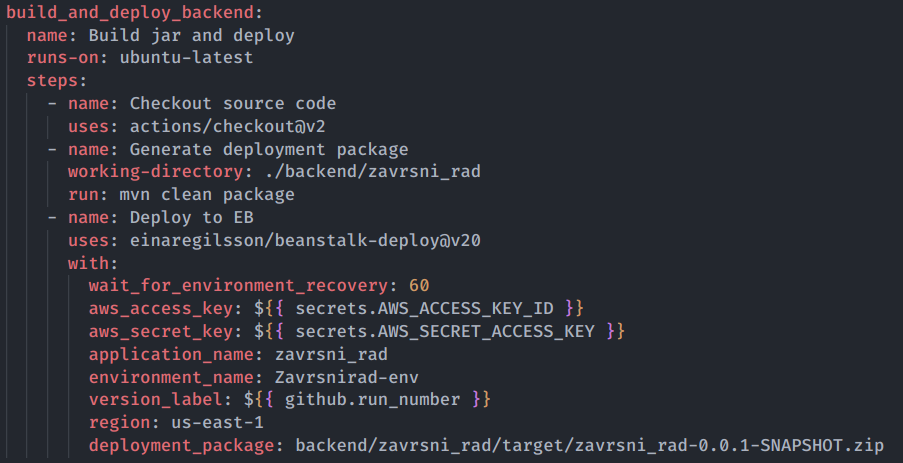
\includegraphics[width=\textwidth]{backend_cicd.png}
      \caption{Github actions zadatak za kontinuiranu isporuku}
      \label{fig:Backend cicd}
\end{figure}
\begin{figure}[h]
      \centering
      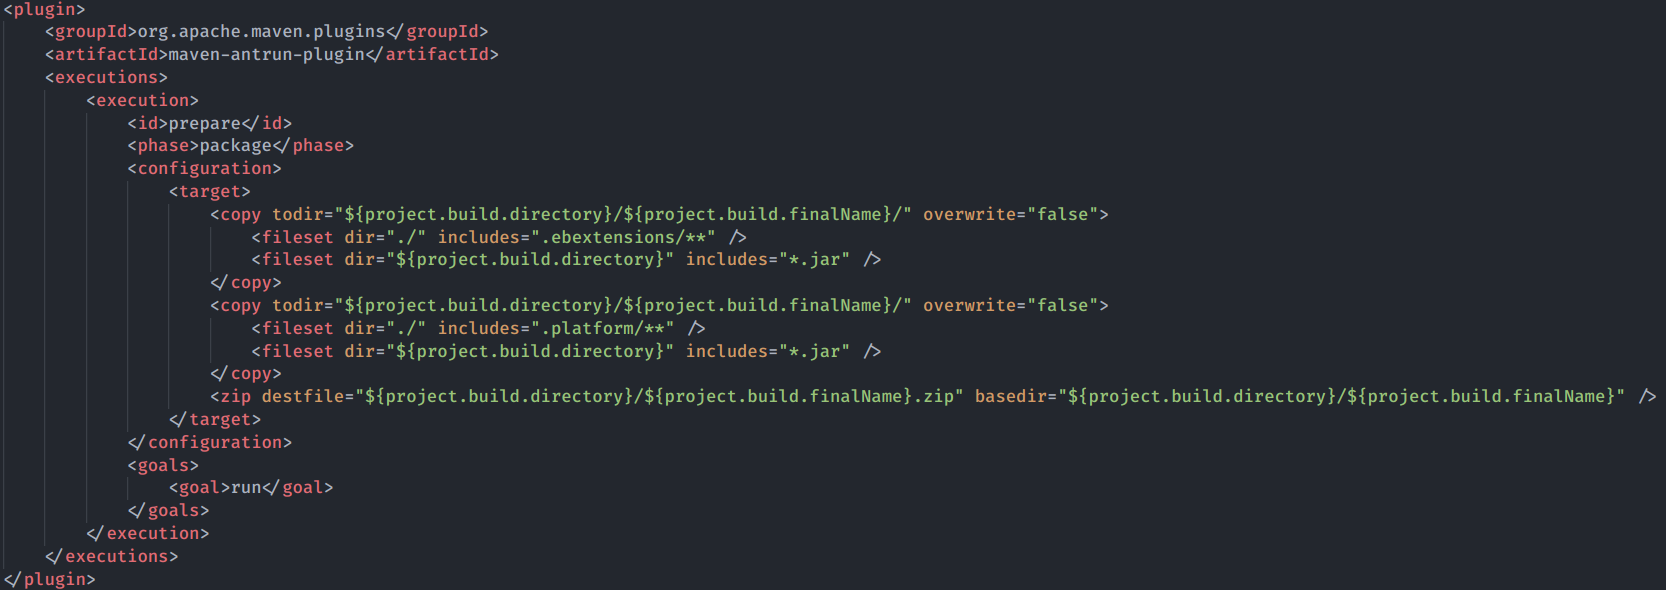
\includegraphics[width=\textwidth]{antrun.png}
      \caption{Plugin za stvaranje zip arhive za upogonjavanje}
      \label{fig:antrun}
\end{figure}

\section{Korisnička strana}
Korisnička strana je pisana u programskom jeziku Dart, pritom koristeći
Flutter radni okvir.
Za komunikaciju s poslužiteljskom stranom korišten je paket \textit{flutter-graphql}.
Za upogonjavanje aplikacije korištena je Github-ova mogućnost
stvaranja izdanja, a sam proces stvaranja je obavljen uz pomoć \textit{Github} akcija (slika \ref{fig:Frontend}).
U svrhe razvoja korišteno je okruženje \textit{VSCode}.
\begin{figure}[h]
      \centering
      \subfloat[\centering GitHub actions za stvaranje nove verzije aplikacije]{{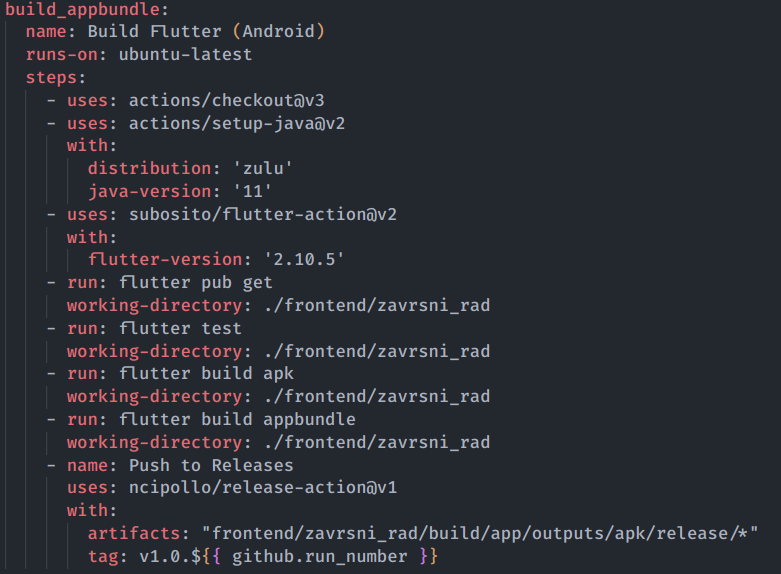
\includegraphics[width=\textwidth]{frontend_cicd.png} }}
      \caption{Osnovne karakteristike korisničke strane}
      \label{fig:Frontend}
\end{figure}

\subsection{Flutter}
Flutter je googleov javno dostupni (\textit{eng. Open Source}) projekt koji je namijenjen
za stvaranje lijepih i brzih mobilnih, web ili računalnih aplikacija. Karakteristika
\textit{Fluttera} je da se aplikacija sa samo jednom napisanim programskim kodom može pokrenuti na
svim navedenim uređajima i na većini operacijskih sustava. Dodatno jedna od prednosti tog radnog okvira je da je vrlo lako napraviti
dinamične aplikacije jer se koristi upravljanje stanjem (eng. \textit{state managment}). Postoji više načina
kako pristupiti ovoj funkcionalnosti, a u ovom radu korištem je \textit{BLoC} obrazac koji je ujedno
i googleov preporučeni način.
\\\\
Sadržaj se isto tako dinamički mijenja u ovisnosti o upitima prema poslužiteljskoj strani i ta dinamičnost
se postiže uz pomoć komponenti namijenjenih za slanje \textit{GraphQL} upita koji se zovu \textit{Query i Mutation}.
Navedene komponente sadrže jednu funkciju koja se poziva svaki put kada se promjeni stanje upita i
zove se \textit{builder}. Toj funkciji se kao ulazni parametar šalje rezultat i stanje izvođenja upita to jest mutacije,
i dužnost joj je vratiti komponentu koja će se prikazati na ekranu.

\subsubsection{BLoC}
BLoC (Business Logic Components) je obrazac za upravljanjem stanjem aplikacije. Karakteristika ovog obrasca
je da međusobno razdvaja prikaz komponente, upravljanje njenim stanjem i logiku iza upravljanja stanjem.
Obrazac je razvijen vodeći se načelom da bi sve asinkrone operacije u aplikaciji trebalo modelirati kao tok događaja. To se
radi na način da jedna komponenta
na osnovu interakcije s okolinom kreira događaje i šalje ih u ulazni tok događaja, a svaka komponenta koja
ovisi o tom toku događaja će kroz izlazni tok primiti bitne podatke i na osnovu njih ažurirati svoje stanje.
\begin{figure}[h]
      \centering
      \subfloat[\centering BLoCProvider i modeli događaja]{{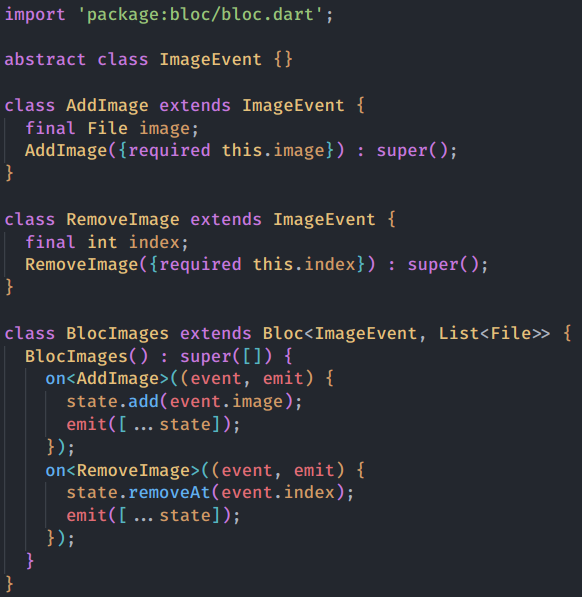
\includegraphics[width=.486\textwidth]{bloc_provider.png} }}
      \subfloat[\centering Primjer BLoCBuilder-a]{{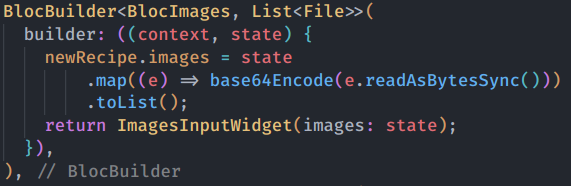
\includegraphics[width=.45\textwidth]{bloc_builder.png} }}
      \caption{Implementacija BLoC-a}
      \label{fig:BLoC}
\end{figure}
U implementaciji se to postiže uz pomoć 3 komponente: prvo su potrebne klase koje predstavljaju događaje (u njima se mogu prenositi
potrebni podaci) (slika \ref{fig:BLoC} (a)), drugo \textit{BlocProvider} (slika \ref{fig:BLoC} (a))
i treće \textit{BlocBuilder} (slika \ref{fig:BLoC} (b)). \textit{BlocProvider} predstavlja dio \textit{BLoC-a}
koji se bavi presretanjem svakog ulaznog događaja, obrađivanjem i slanjem u izlazni tok, a \textit{BlocBuilder}
služi za izgradnju komponente na osnovu trenutnog događaja u izlaznom toku događaja.

\subsection{Implementacija ekrana u \textit{flutter-u}}
U radnom okviru \textit{Flutter} ne postoji razlika između primjerice ekrana (eng \textit{screen}) i teksta jer je sve definirano
kao komponenta (eng. \textit{"widget"}), ali iz semantičkih razloga svaku skupinu komponenti koja
se prikazuje u istome trenutku nazivamo ekran. Često se broj ekrana uzima kao stupanj
složenosti aplikacije. Tako ovaj rad ima 9 ekrana, ali oni nisu dostupni svim korisnicima nego
su podijeljeni po ulogama.

\subsubsection{Ekran dobrodošlice i prijave}
Karakteristika ekrana dobrodošlice je
da se prikazuje samo jednom prilikom prvog pokretanja aplikacije
uređaju. To svojstvo se postiže podizanjem zastavice u memoriji uređaja uz pomoć
sučelja dijeljenih tajni (eng. \textit{"SharedPreferences"}).
Ekran za prijavu sadrži 2 polja za unos i 3 gumba (slika \ref{fig:WelcomeLogin} (b)). Prvo polje je polje za unos
korisničkog imena ili e-pošte, drugo polje je polje za unos pripadajuće lozinke. Ako je uneseno
krivo korisničko ime ili lozinka prikazuje se odgovarajuća poruka (slika \ref{fig:WelcomeLogin} (c)). Preostali gumbovi su
gumb za preskakanje prijave i prelazak na stranicu sa svim receptima, gumb
za potvrdu prijave koji šalje zahtjev za prijavu na poslužitelj te gumb za prelazak na ekran za registraciju.

\subsubsection{Ekran za registraciju}
Ekran za registraciju sadrži 5 polja za unos: unos računa elektroničke pošte,
korisničkog imena, lozinke, potvrda lozinke i odabir profilne slike. Profilna slika je, za
razliku od ostalih polja, opcionalno polje. Karakteristika polja za lozinku je da ima posebne
validacijske kriterije. Ti kriteriji zahtjevaju da lozinka mora
sadržavati barem 8 znakova, jedno veliko slovo i jedan specijalni znak.
Nakon uspješne registracije
prikaže se poruka o uspješnoj registraciji (slika \ref{fig:Register} (b)) i da je potrebno izvršiti potvrdu identiteta
putem e-mail računa koji je bio unesen. Ukoliko je registracija nevaljana prikaže se odgovarajuća poruka (slika \ref{fig:Register} (a)).

\subsubsection{Ekran za pregled svih recepata}
Ekran za pregled svih recepata će uvijek biti prvi ekran koji će se prikazati ako postoji
prijavljeni korisnik, a to se također postiže uz pomoć dijeljenih tajni \textit{(eng. SharedPreferences)}.
Ekran za pregled svih recepata se razlikuje u navigacijskoj traci, ovisno o ulozi koja je dodijeljena trenutno prijavljenom korisniku.
Naime traka sadržava samo one gumbe koji vode do ekrana koji su dozvoljeni
trenutno prijavljenom korisniku (slika \ref{fig:tracks}).
\begin{figure}[h]
      \centering
      \subfloat[\centering Traka za neprijavljenog korisnika]{{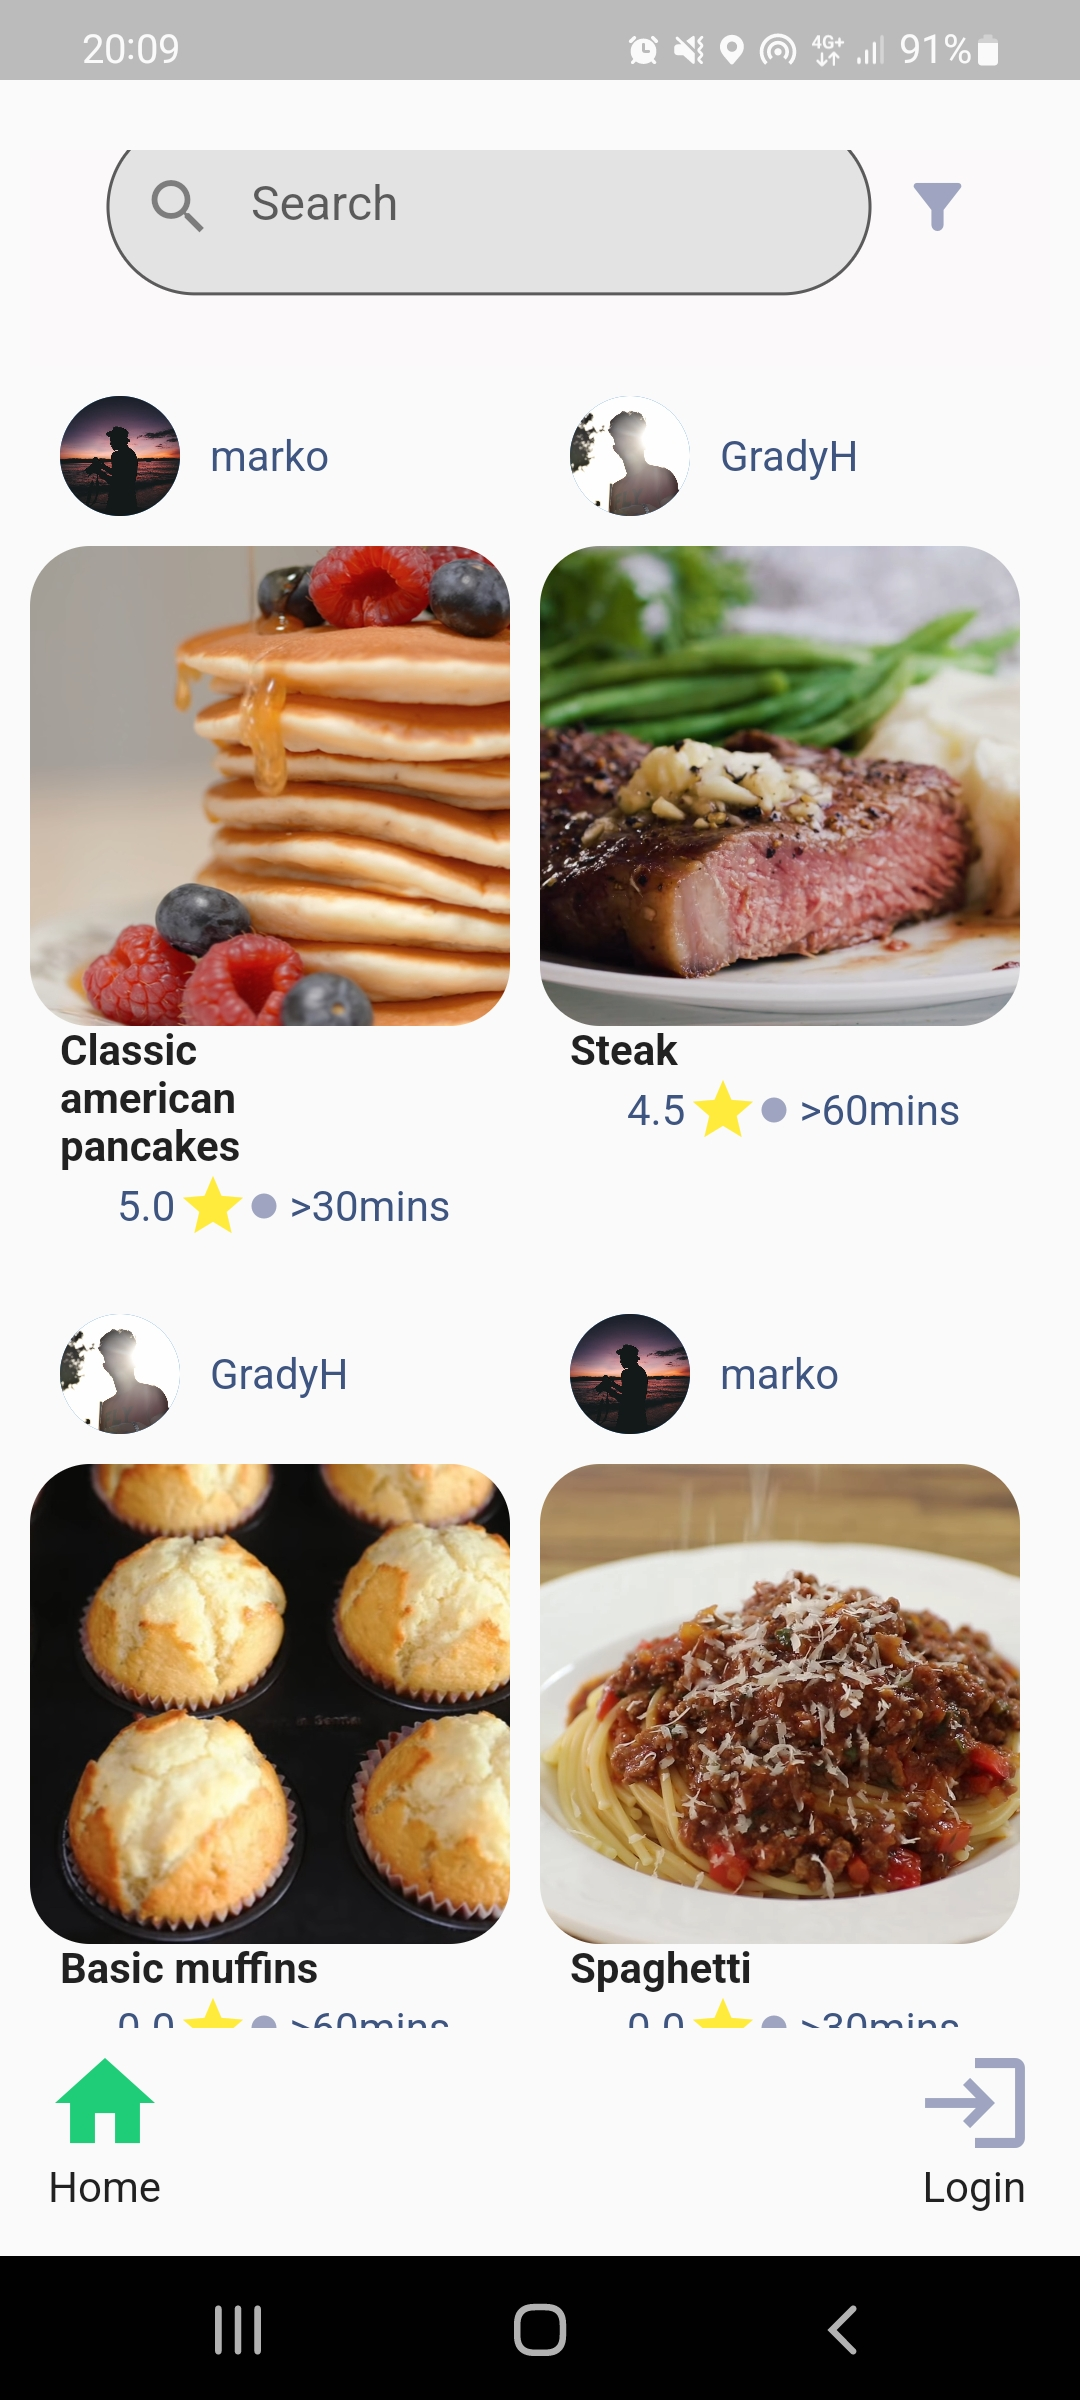
\includegraphics[width=.25\textwidth]{not_loggedin.jpg} }}
      \subfloat[\centering Traka za prijavljenog korisnika]{{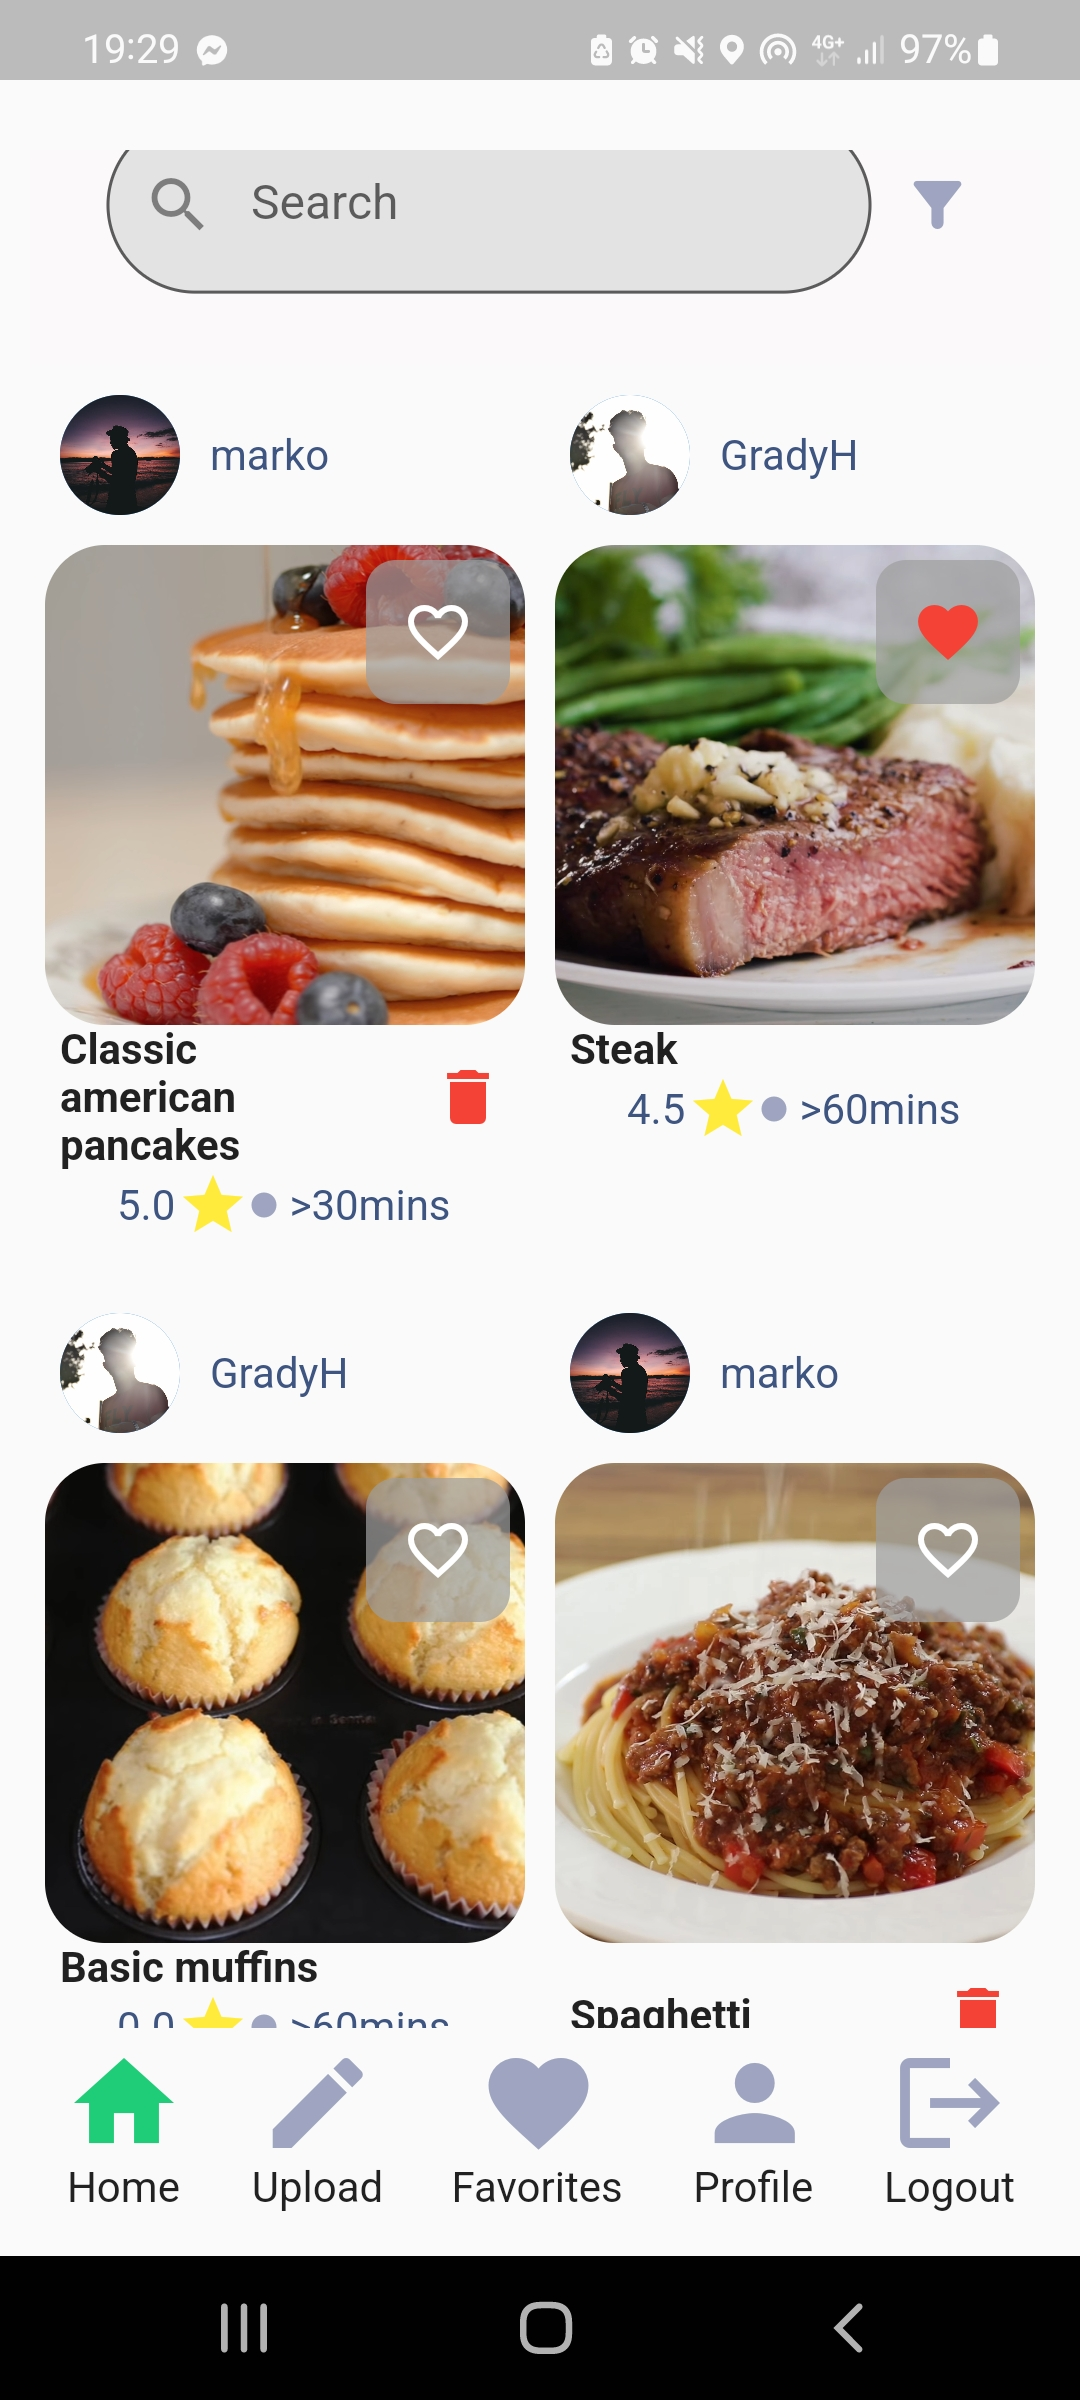
\includegraphics[width=.25\textwidth]{user_all_recipes.jpg} }}
      \subfloat[\centering Traka za administratora]{{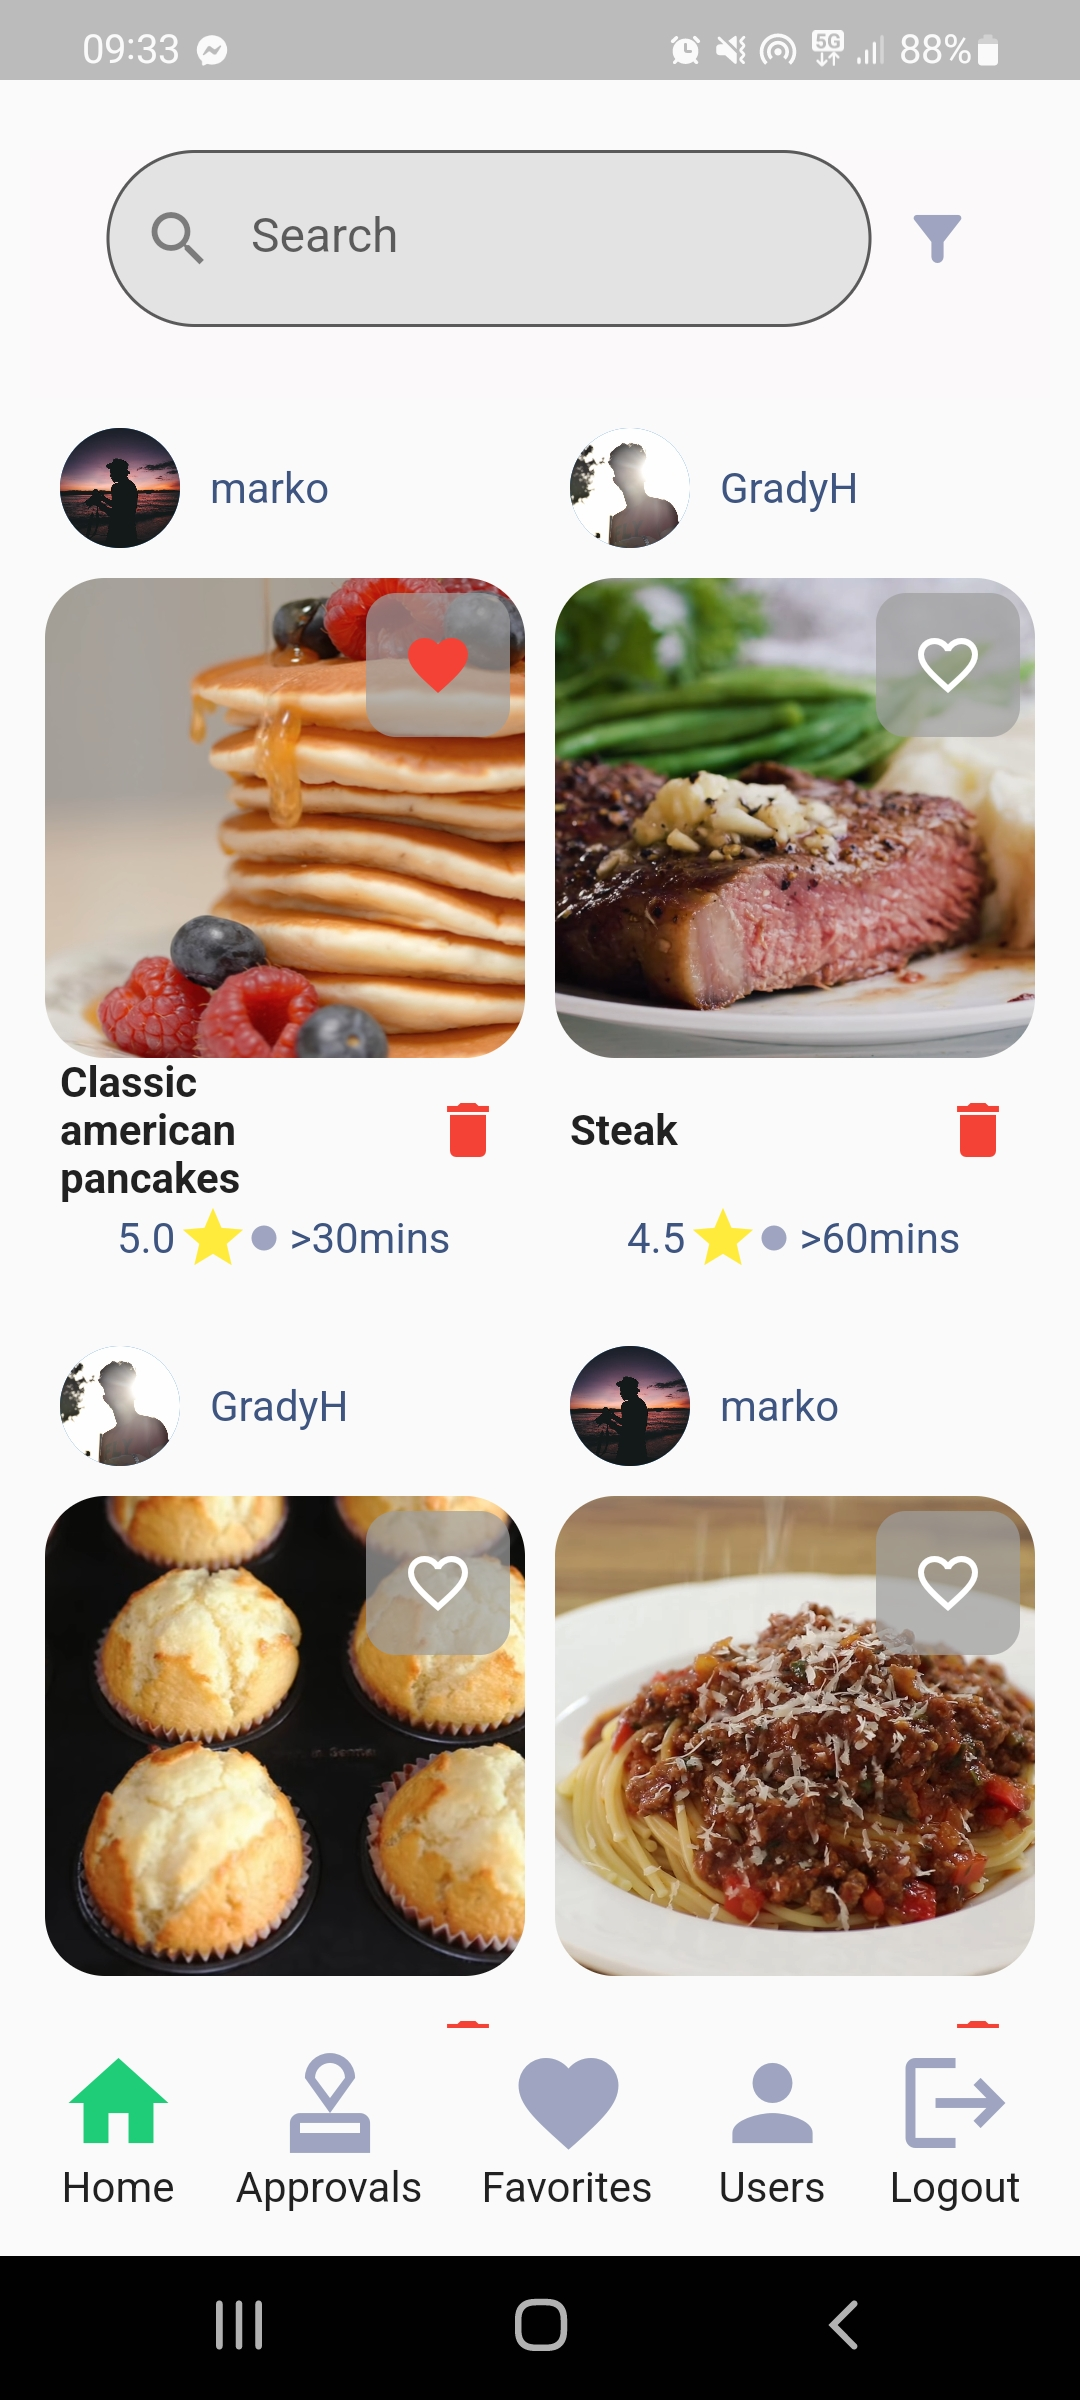
\includegraphics[width=.25\textwidth]{admin_allrecipes.jpg} }}
      \caption{Različite trake za različite korisnike}
      \label{fig:tracks}
\end{figure}
\\\\
Trenutno prijavljeni korisnik se određuje na temelju dijeljenjih tajni.
U njih se spremaju podaci o trenutnom korisniku, kao na primjer korisničko ime, identifikacijski
broj i \textit{JWT token} za autentifikaciju i autorizaciju.
To je bitno jer će se prije svakog upita, koji se obavlja daljnjom interakcijom
korisnika i aplikacije, u HTTP zaglavlje staviti spomenuti token. Uz pomoć tog tokena će
poslužiteljska strana obaviti autentifikaciju i autorizaciju. Ako korisnik ne bude uspješno
autoriziran biti će odjavljen i preusmjeren na ekran za prijavu s odgovarajućom porukom.
\\\\
Recepti su podijeljeni u stranice,
a svaka stranica sadrži 10 recepata. Ako postoji više od 10 recepata na dnu ekrana će se pojaviti
jedna komponenta koja služi za prelazak na sljedeću, prethodnu ili neku određenu stranicu.
Za svaki recept naveden je autor i profilna slika autora, pozadinska slika recepta, naziv,
prosječna ocjena i vrijeme potrebno za pripremu. Klikom na bilo koji opisnik recepta otvara se novi ekran
za pregled pojedinog recepta. U gornjem desnom kutu opisnika postoji
gumb za dodavanje recepta u favorite. U donjem desnom kutu opisnika postoji gumb koji služi za brisanje recepta koji
je prikazan samo u slučaju da recept pripada trenutno prijavljenom korisniku ili je trenutno prijavljeni
korisnik administrator.
\\\\
Također, na samom vrhu ekrana postoji komponenta koja služi za filtriranje recepata po nazivu,
a pored njega se nalazi jedan gumb koji prilikom dodira otvara prozorčić koj
omogućava filtriranje recepata po sastojcima i vremenu pripreme.


\subsubsection{Ekran za pregled pojedinog recepta}
Ekran za pregled pojedinog recepta će prikazivati sve podatke o receptu, a to su:
sastojci, koraci pripreme, svi videozapisi i fotografije
koje se nalaze u pomičnoj listi s kojom se interagira pokretima lijevo i desno. Dodatno, ako
trenutno prijavljeni korisnik ima dovoljne ovlasti moći će kliknuti na gumb za ocjenjivanje i
vidjeti polje za unos komentara. Ako je prijavljeni korisnik administrator moći će kliknuti na
gumb za odobravanje, to jest poništavanje odobrenja recepta (slika \ref{fig:New recipe} (c) i (d)).


\subsubsection{Ekran za dodavanje novog recepta}
Ekran za dodavanje novog recepta dostupan je samo prijavljenim korisnicima koji nisu administratori.
Ovaj ekran sastoji se od velikog broja polja za unos i odabir videozapisa i fotografija te gumba za potvrdu.
Karakteristika svakog polja je da ne smije biti prazno i ne smije sadržavati više znakova od broja koji
je određen bazom podataka. Posebne sekcije su sekcije za unos sastojaka, koraka pripreme, videozapisa i
fotografija jer su one modelirane BLoC obrascem. To je potrebno jer nije moguće unaprijed znati koliko
takvih objekata korisnik želi dodati, stoga postoji opcija za dinamičko dodavanje
polja za unos (slika \ref{fig:New recipe} (a) i (b)).

\subsubsection{Ekran za upravljanje korisnicima}
Posljednji ekran je ekran za upravljanje korisnicima, on je dostupan samo administratorima. Na ovoj stranici nalazi se
popis svih korisnika, a straničenje funkcionira na potpuno jednak način kao i straničenje za recepte.
Za svakog korisnika navedeno je korisničko ime, profilna slika i gumb za suspendiranje, to jest
poništavanje suspenzije. Nema opcije za brisanje korisnika jer bi to značilo da bi pojedini recepti
ostali bez autora ili bi bili obrisani iz baze što nije poželjna funkcionalnost. Zato je korinsiku koji je suspendiran
samo onemogućena prijava u sustav (slika \ref{fig:Single recipe} (a)).

\chapter{Upute za instalaciju i pokretanje rješenja}
Preduvjet za instalaciju aplikacije je posjedovanje Android uređaja jer je aplikacija namijenjena samo
za takve uređaje. Za instalaciju potreban je instalacijski paket koji je moguće preuzeti iz jednog od izdanja
na: \href{https://github.com/MarkoTunjic/Final-BSc-Thesis}{github.com/MarkoTunjic}. Prije pokretanja
procesa instalacije potrebno je u postavkama mobitela odobriti instalaciju iz nepoznatih izvora jer aplikacija
nije odobrena od strane \textit{Google play-a}. Kada instalacija završi aplikacija je spremna za uporabu.
\\\\
Poslužiteljsku stranu i bazu podataka nije potrebno pokretati jer su već pokrenute u \textit{"oblaku"}.

\chapter{Zaključak}
Konačni proizvod ovoga rada je potpuno funkcionalna mobilna aplikacija koja je globalno dostupna u svakom trenutku.
Aplikacija se sastoji od 3 dijela: baze podataka, poslužiteljski dio i korisnički dio. Svaki od njih funkcionira potpuno
samostalno i neovisno o ostalim dijelovima. Svaki dio ima neke prednosti i nedostatke koje je potrebno
nadograditi u budućim radovima.
\\\\
Prednost baze podataka je što se slike i videozapisi spremaju kao hiperveze
jer to održava veličinu baze najmanje mogućom. To je postignuto na način da se fotografije i videozapisi
spremaju u "oblak" točnije \textit{Firebase}. Nedostatak
je taj što se ne koriste pohranjene procedure koje bi bilo korisno implementirati
u budućim radovima jer bi to dodatno olakšalo i osiguralo proces dohvata podataka.
\\\\
Poslužiteljska strana ima prednost jer je implementirana GraphQL
arhitekturnim stilom koji smanjuje gomilanje prijenosnih objekata i krajnjih točaka. Uz to rješava problem
prekomjernog i nedovoljnog dohvata podataka.
Mana je ta što se ne obavlja provjera pristiglih fotografija i videozapisa prije slanja na \textit{Firebase} čime je
je sigurnost aplikacije narušena. Ovo nužno mora biti popravljeno u budućim verzijama rada.
\\\\
Velika prednost korisničke strane je što se za upravljanje stanjem koristio
\textit{BLoC} obrazac koji je brz i razdvaja logiku obrade događaja od prikaza komponenti.
Time je aplikacija prikladno uslojena i oblikovana po SOLID načelima. Nedostatak je taj što nisu implementirane
obavijesti. Dakle, korisnici neće primati obavijesti ukoliko je netko ocjenio ili komentirao njihov recept, a administratori neće
primiti obavijest ukoliko neki korisnik doda novi recept. Ova funkcionalnost bila bi korisna za implementirati
jer bi poboljšala iskustvo prilikom korištenja aplikacije.

\bibliography{literatura}
\bibliographystyle{fer}
\nocite{ProgramiranjeUJavi}
\nocite{GraphQL}
\nocite{Authentication}
\nocite{Spring}
\nocite{bloc}

\begin{sazetak}
      U ovom radu napravljena je mobilna aplikacija koja će krajnjim korsinicima olakšati spremanje i pretraživanje
      recepata. Aplikacija se sastoji od 3 dijela: baze podataka, poslužiteljske strane i korisničke strane.
      Da bi aplikacija svima i u svakom trenutku bila dostupna korištene su usluge u oblaku od tvrtke Amazon.
      Baza podataka je implementirana kao relcijska baza podataka, a kao upravitelj je korišten PostgreSQL.
      Za razvoj poslužiteljske strane korišten je radni okvir SpringBoot. Kao arhitekturni stil je korišten GraphQL.
      GraphQL predstavlja upitni jezik namijenjen korisničkoj strani za dohvat samo onih podataka
      koji su uistinu potrebni.
      Korisnička strana je implementirana u flutter radnom okviru. Jedna od prednosti tog radnog okvira je da se
      temelji na nativnom (eng. native) pristupu razvoju aplikacija. Takav pristup omogućava pisanje samo jednog izvornog koda koji će se moći pokrenuti
      na većini operacijskih sustava.
      \kljucnerijeci{Mobilna aplikacija, baza podataka, poslužiteljska i korisnička, PostgreSQL, SpringBoot, GraphQL, Flutter, AWS .}
\end{sazetak}
% TODO: Navedite naslov na engleskom jeziku.
\engtitle{Mobile application for recipe managment}
\begin{abstract}
      The result of this project is a mobile application that will help the end users store and search for recipes.
      The aplication is divided in three parts: database, backend and frontend. In order for the application
      to be globally and constantly accessible cloud services made by the company Amazon were used.
      The database is implemented as a relational databse and PostgreSQL was used as the database manager.
      The framework used to develop the backend is SpringBoot. The architectural style that was used is GraphQL.
      GraphQL is a query language intended to be used on the frontend to fetch only the required data.
      The frontend was implemented using the Flutter framework. One of the benefits of that framework is that it uses
      a native approach to development. Such an approach enables writing a single codebase which can be run
      on nearly every operating system.

      \keywords{Mobile application, database, backend, frontend, PostgreSQL, SpringBoot, GraphQL, Flutter, AWS.}
\end{abstract}

\end{document}
